\documentclass[12pt,a4paper]{report}

\usepackage[top=2cm, bottom=2cm, left=2cm, right=2cm]{geometry}
\usepackage{silence}

\usepackage[latin1]{inputenc}
\usepackage[T1]{fontenc}
\usepackage[francais]{babel}
\usepackage{layout}

\usepackage{array}
\usepackage{amsmath}
\usepackage{amsthm}
\usepackage{amsfonts}
\usepackage{amssymb}
\usepackage{mathrsfs}
\usepackage{mathtools}
\usepackage{titlesec}
\usepackage{enumerate}

\usepackage{frcursive} % --------------- �criture manuscrite
\usepackage{marvosym} % --------------- \Capricorn - espace topologique
\usepackage[dvipsnames]{xcolor}
\usepackage{graphicx}
\usepackage[dvips]{epsfig,psfrag}



\usepackage{array}
\usepackage{amsmath}
\usepackage{amsthm}
\usepackage{amsfonts}
\usepackage{amssymb}
\usepackage{mathrsfs}
\usepackage{mathtools}

\usepackage{frcursive} % --------------- �criture manuscrite
\usepackage{marvosym} % --------------- \Capricorn - espace topologique

\renewcommand{\emptyset}{\varnothing}
\newcommand{\calligraphic}[1]{\raisebox{-.4ex}{\cursive{\textcal #1}}}
\newcommand{\Tau}{\text{\Capricorn}}
\newcommand{\maps}{\rightarrow}
\newcommand{\ssi}{\Leftrightarrow}
\newcommand{\inv}[1]{{#1}^{-1}}
\newcommand{\adj}[1]{{#1}^{t}}
\newcommand{\biadj}[1]{{#1}^{tt}}
\newcommand{\ortho}{^\perp}
\newcommand{\dual}{^\star}
\newcommand{\bidual}{^{\star\star}}
\newcommand{\tridual}{^{\star\star\star}}
\newcommand{\abs}[1]{\left\vert{#1}\right\vert}
\newcommand{\norme}[1]{\left\Vert{#1}\right\Vert}
\newcommand{\triplenorme}[1]{\abs{\abs{\abs{#1}}}}
\newcommand{\scal}[2]{\left\langle {#1} \middle| {#2} \right\rangle}
\newcommand{\conj}[1]{\overline{#1}}
\newcommand{\adh}[1]{\overline{#1}}
\newcommand{\weak}[1]{\sigma({#1}, {#1}\dual)}
\newcommand{\pweak}[1]{\sigma({#1}\dual, {#1})}
\newcommand{\restrictions}[2]{{#1}_{|_{#2}}}
\newcommand{\James}[1]{\mathcal{J}_{#1}}
\newcommand{\normeJames}[2]{\norme{#2}_{\James{p}}}
\newcommand{\normeJamesB}[2]{\norme{#2}_{\James{p}\bidual}}
\newcommand{\normeJamesI}[2]{\triplenorme{#2}_{\James{p}}}
\newcommand{\normeJamesIB}[2]{\triplenorme{#2}_{\James{p}\bidual}}

%\newenvironment{Preuve}[1][]{\subsubsection*{Preuve #1}}{\vspace{-1em}\begin{flushright}$\square$\end{flushright}}

\DeclareMathOperator{\e}{e}
\DeclareMathOperator{\codim}{codim}
\DeclareMathOperator{\conv}{conv}
\DeclareMathOperator{\convAdh}{\adh{conv}}
\DeclareMathOperator{\dist}{dist}
\DeclareMathOperator{\Span}{span}
\DeclareMathOperator{\Arg}{Arg}
\DeclareMathOperator{\Image}{Im}
\DeclareMathOperator{\SpanAdh}{\adh{span}}

\renewcommand{\newline}{\vspace{\baselineskip}}
\newcommand{\delline}{\vspace{-\baselineskip}}


\newtheorem{Thm}{Th�or�me} [chapter]
\newtheorem{Def}[Thm]{D�finition}
\newtheorem{Rem}[Thm]{Remarque}
\newtheorem{Prop}[Thm]{Proposition}
\newtheorem{Lemme}[Thm]{Lemme}
\newtheorem{Corol}[Thm]{Corollaire}
\newtheorem{Rappel}[Thm]{Rappel}

\titleformat\chapter[hang]{\normalfont\huge\bfseries}{\thechapter}{1em}{}

\newcommand{\chapterref}{\section*{R�f�rences pour ce chapitre}}

%\includeonly{intro}

\begin{document}
\scrollmode

    \title{\bf\Huge{Espaces r�flexifs}}
\author{Poulain Julien}

\maketitle
    \tableofcontents
    
    \addtocounter{chapter}{-1}

\chapter{Introduction}

Comme probablement de nombreux �tudiants avant moi, et bien plus apr�s moi, je me suis demand� {"\textit{Qu'est-ce que ces espaces ont de si particulier, si ce n'est une fonction particuli�re qui devient surjective?}"} lorsqu'� l'un de mes cours j'ai appris ce qu'�tait un espace r�flexif. Ce m�moire a pour but d'apporter une r�ponse � cette question, en montrant principalement qu'un espace r�flexif repr�sente bien plus qu'une fonction surjective.

On aura l'occasion de se rendre compte qu'il est �troitement li� � de nombreux concepts relatifs aux espaces de Banach, � commencer par le fait que tout espace r�flexif est complet. C'est pourquoi dans l'int�gralit� de ce travail, on consid�rera toujours un espace de Banach $E$ non nul, sauf mention contraire.

On verrons dans un premier temps une s�rie d'exemples d'espaces r�flexifs, ainsi que certaines propri�t�s �l�mentaires de ceux-ci. Dans un second temps on �tudiera, tout au long des diff�rents chapitres, de multiples caract�risations de la r�flexivit�. Les premi�res concerneront les diff�rentes topologies de l'espace ainsi que la compacit� de sa boule unit�, alors que d'autres exigeront certaines propri�t�s � ses �ventuelles bases de Schauder.

On donnera �galement certains crit�res permettant de d�terminer si un espace est r�flexif ou non. D'une part, l'existence d'une suite d'un type particulier implique que l'espace n'est pas r�flexif. D'autre part, pour peu que l'on ait trouv� une base de Schauder suffisament puissante, il suffit de d�montrer que l'espace ne contient aucune copie de $c_0$ ou de $l^1$ pour en d�duire qu'il est r�flexif.

Pourtant, les deux espaces cit�s ne sont pas les seuls espaces non r�flexifs, ils sont en fait tr�s nombreux. On proposera alors un exemple d'espace non r�flexif assez caract�ristique. Sa principale particularit� vient du fait qu'il est presque aussi gros que son bidual, c'est-�-dire qu'il n'y a qu'une seule dimension d'�cart entre les deux. Nous changerons alors de norme pour une �quivalente � la pr�c�dente, et constaterons qu'elle rend l'espace isom�trique � son bidual.

    
\chapter{Dual, bidual et r�flexivit�}

\section{Rappels, d�finitions, propri�t�s �l�mentaires}

Soient $E$ et $F$ deux espaces vectoriels norm�s. On d�finit l'espace vectoriel
\[
\mathscr{L}(E, F) = \{f:E\maps F\text{ lin�aire continue}\}
\]
muni de la norme
\[
\norme{T} = \sup_{x\in B(E)}\norme{T(x)} ~~~~~~~~\text{pour } T\in\mathscr{L}(E, F)
\]

\begin{Prop}
$\mathscr{L}(E, F)$ est complet $\ssi F$ est complet.
\end{Prop}

On d�signera le dual topologique de $(E, \norme{.})$ par $E\dual=\mathscr{L}(E, \mathbb{K})$, qui est un espace de Banach. De la m�me fa�on, on d�signera le bidual topologique de $(E, \norme{.})$ par $E\bidual = \mathscr{L}(E^*, \mathbb{K})$.

On peut imm�diatement identifier une cat�gorie particuli�re d'�l�ments du bidual. Soit $x\in E$. On d�finit
\[
\begin{array}{lllll}
ev_x&:&E\dual&\maps&\mathbb{K}\\
&:&x\dual&\mapsto&x\dual(x)
\end{array}
\]
l'�valuation en $x$ des fonctionnelles de $E$. On d�montre ais�ment que $ev_x\in E\bidual$, et on peut d�s lors d�finir l'application lin�aire
\[
\begin{array}{lllll}
i&:&E&\maps&E\bidual\\
&:&x&\mapsto&ev_x
\end{array}
\]
Cette application est en fait une isom�trie, c'est-�-dire que pour tout $x\in E, \norme{i(x)}=\norme{x}$. En effet,
\[\norme{i(x)} =
\sup_{x\dual\in B(E\dual)}\abs{x\dual(x)} \leqslant
\norme{x}\]

De plus, si on note $x_0\dual$ l'�l�ment donn� par le th�or�me de Hahn-Banach (\ref{HBF}), on a

\[
\norme{i(x)} =
\sup_{x\dual\in B(E\dual)}\abs{x\dual(x)} \geqslant
\abs{x_0\dual(x)} = \norme{x}
\]

De ceci, et du fait que $i$ est lin�aire, on d�duit qu'elle est aussi continue et injective. On appellera $i$ l'injection canonique de $E$ dans son bidual.

\begin{Def}
On dit que $E$ est r�flexif si son injection canonique est surjective.
\end{Def}

\begin{Prop}
Si $E$ est r�flexif, alors $E$ est complet et $i$ est bicontinue.
\end{Prop}
\begin{proof}
En effet, $i$ �tant une bijection lin�aire, $i^{-1}$ est aussi une bijection lin�aire. De plus, le fait que $i$ est une isom�trie implique qu'elle est bicontinue. Dans ce cas, puisque $i(E) = E\bidual$, et que $E\bidual$ est complet, on en d�duit que $E$ l'est aussi.
\end{proof}

\subsubsection*{Exemples}
\begin{itemize}
\item Soit $E$ un espace vectoriel norm� de dimension finie. Toute application lin�aire de $E$ dans $\mathbb{K}$ est continue, donc son dual topologique et son dual alg�brique sont �gaux. On sait aussi que le dual alg�brique a m�me dimension que $E$, donc $\dim(E)=\dim(E\bidual)$. L'application $i:E\maps E\bidual$ �tant injective, elle est aussi surjective. Donc $E$ est r�flexif.
\item Pour $p, q\in~]1,+\infty[$ tels que $\frac{1}{p}+\frac{1}{q}=1$, l'espace $l^p$ est r�flexif, et $(l^p)\dual=l^q$.
\item L'espace $c_0$ n'est pas r�flexif, puisque $c_0\dual=l^1$, $(l^1)\dual=l^\infty$, et $c_0\neq l^\infty$.
\item L'espace $c_{00}$ n'est pas r�flexif, puisqu'il n'est pas complet.
\item � titre d'exemple, on a le corollaire du th�or�me suivant:
\end{itemize}

\begin{Thm}[Riesz-Fr�chet]\label{rieszfrechet}
Soit $H$ un espace de Hilbert. Alors toute forme lin�aire continue sur $H$ s'�crit de mani�re unique comme un produit scalaire o� l'une des deux variables est fix�e. Plus formellement
\[\forall x\dual\in H\dual, \exists \: ! \: x\in H\text{ tel que }\norme{x}=\norme{x\dual}\text{ et }\forall y\in H, x\dual(y)=\scal{y}{x}\]
\end{Thm}
\begin{Corol}
Tout espace de Hilbert est r�flexif.
\end{Corol}
\begin{proof}
Soient $H$ un espace de Hilbert et $x\bidual\in H\bidual$. Par le th�or�me de Riesz-Fr�chet, l'application anti-lin�aire
\[
\begin{array}{lllll}
l&:&H&\maps&H\dual\\
&:&y&\mapsto&\left(
    \begin{array}{lllll}
    l_y&:&H&\maps&\mathbb{K}\\
    &:&x&\mapsto&\scal{x}{y}
    \end{array}
\right)
\end{array}
\]
est une isom�trie bijective. Par cons�quent, $\conj{x\bidual\circ l}\in H\dual$.
On lui applique le th�or�me de Riesz-Fr�chet, il existe $x\in H$ tel que $\norme{x}=\norme{\conj{x\bidual\circ l}}=\norme{x\bidual}$ et $\conj{x\bidual\circ l}(y) = \scal{y}{x}=\conj{\scal{x}{y}}$, pour tout $y\in H$. On a donc que pour tout $y\in H, x\bidual(l_y) = (x\bidual\circ l)(y) = \scal{x}{y} = l_y(x)$, d'o� $x\bidual=ev_x$ et $i$ est surjective.
\end{proof}



Ceci constitue d�j� une grande cat�gorie d'espaces r�flexifs. Il serait int�ressant � ce stade de savoir s'il existe une certaine stabilit� dans la classe des espace r�flexifs, et si oui, de quelle nature. C'est ce � quoi on va s'affairer dans cette section.

\begin{Def}
Soient $E$ et $F$ deux espaces de Banach, et $T:E\maps F$ une application lin�aire continue. L'ajointe de $T$ est not�e $\adj{T}$ et d�finie par

\[
\begin{array}{lllll}
\adj{T}&:&F\dual&\maps&E\dual\\
&:&y\dual&\mapsto&y\dual\circ T
\end{array}
\]

De plus, c'est une application lin�aire continue et $\norme{\adj{T}}=\norme{T}$.
\end{Def}

\begin{Prop}\label{isoreflex}
Soient $E$, $F$ deux espaces vectoriels norm�s isomorphes via $T:E\maps F$. Alors

\begin{enumerate}[(1)]
\item L'application $\adj{T}$ est un isomorphisme
\item Si $E$ est r�flexif, alors $F$ aussi
\end{enumerate}
\end{Prop}
\begin{proof}
~

(1)\\
%
Puisque $\adj{T}$ est continue, il suffit de montrer que c'est une bijection et le th�or�me des isomorphismes de Banach nous donnera la continuit� de l'inverse.

$\adj{T}$ est injective:\\
%
Soit $y\dual\in F\dual$ tel que $\adj{T}(y\dual)=0$. On a que $y\dual(T(x))=0$ quelque soit $x\in E$. Puisque $T$ est bijective, c'est �quivalent � dire que $y\dual(y)=0$ quelque soit $y\in F$, c'est-�-dire que $y\dual=0$.\newline

$\adj{T}$ est surjective:

Soit $x\dual\in E\dual$. On prend $y\dual=x\dual\circ\inv{T}\in F\dual$. Soit $x\in E$, alors

\[
T\dual(y\dual)(x)
=
y\dual(T(x))
=
x\dual(\inv{T}(T(x)))
=
x\dual(x)
\]

D'o� $x\dual=\adj{T}(y\dual)$.\newline

(2)\\
%
Soit $y\bidual\in F\bidual$. Puisque $T$ est un isomorphisme, on sait par (1) que $\biadj{T}$ est �galement un isomorphisme. De plus, $E$ est r�flexif, par cons�quent il existe $x\in E$ tel que $\biadj{T}(ev_x) = y\bidual$. Soit $y\dual\in F\dual$. On a

\[
y\bidual(y\dual)
=
ev_x(\adj{T}(y\dual))
=
(\adj{T}(y\dual))(x)
=
y\dual(T(x))
=
ev_{T(x)}(y\dual)
\]

D'o� $y\bidual=ev_{T(x)}$, donc $F$ est r�flexif.
%\raisebox{-0.6\height}{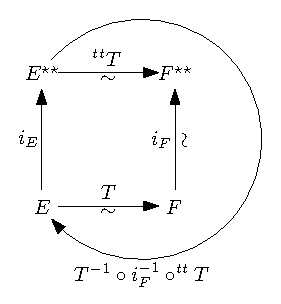
\includegraphics[scale=1]{rappels/diagrammeisodual.eps}}
\end{proof}




\begin{Prop}\label{equivreflexif}
Les assertions suivantes sont �quivalentes:
\begin{enumerate}[(1)]
\item $E$ est r�flexif
\item $E\dual$ est r�flexif
\item tout sous-espace vectoriel ferm� de $E$ est r�flexif
\end{enumerate}
\end{Prop}
\begin{proof}
(1) $\Rightarrow$ (2)\\
Notons $i$ l'injection canonique de $E$, et $j$ l'injection canonique de $E\dual$. On veut montrer que $j$ est surjectif. Puisqu'on a l'injectivit�, cela revient � d�montrer que $j$ est bijective, et donc de mani�re �quivalente qu'il admet un inverse. Pour ce faire, on va montrer que $\adj{i}$ est l'inverse de $j$. Pour cela, il suffira de v�rifier que \hbox{$j\circ\adj{i}=Id_{E\tridual}$}.

Soient $x\tridual\in E\tridual$ et $x\bidual\in E\bidual$. Puisque $E$ est r�flexif, il existe $x\in E$ tel que $i(x)=x\bidual$. On calcule
\[
j(\adj{i}(x\tridual))(x\bidual)=
x\bidual(\adj{i}(x\tridual))=
ev_x(\adj{i}(x\tridual))=
\adj{i}(x\tridual)(x)=
x\tridual(i(x))=
x\tridual(x\bidual)
\]
Qui se traduit par
\[
\begin{array}{l}
\forall x\tridual\in E\tridual, \forall x\bidual\in E\bidual, j(\adj{i}(x\tridual))(x\bidual)=x\tridual(x\bidual)\\
\Rightarrow \forall x\tridual\in E\tridual, j(\adj{i}(x\tridual))=x\tridual\\
\phantom{\Rightarrow} \Rightarrow j\circ\adj{i}=Id_{E\tridual}\\
\end{array}
\]

Par cons�quent, $\adj{i}$ est bien l'inverse de $j$, donc $j$ est surjectif et $E\dual$ r�flexif.\newline

(1) $\Rightarrow$ (3)\\
Puisque $F$ est ferm�, l'application lin�aire
\[
\begin{array}{lllll}
\pi&:&E\dual&\maps&F\dual\\
&:&x\dual&\mapsto&\restrictions{x\dual}{F}
\end{array}
\]
est bien d�finie et continue. Le th�or�me de Hahn-Banach (\ref{HBA}) dit exactement que cette application est surjective:

Soit $y\bidual\in F\bidual$. Alors $y\bidual\circ\pi\in E\bidual$. Comme $E$ est r�flexif, il existe $x\in E$ tel que $ev_x=y\bidual\circ\pi$. Pour montrer que $x\in F$, on proc�de par l'absurde. Dans ce cas, le th�or�me de Hahn-Banach (\ref{HBA}) affirme qu'il existe une fonctionnelle continue $x\dual\in E\dual$ qui s'annule sur $F$ mais pas en $x$. Alors, on a que
\[
ev_x(x\dual)
=
y\bidual(\pi(x\dual))
=
0
\]
Ce qui est absurde. Par cons�quent, $x\in F$. Alors quelque soit $x\dual\in E\dual$, on a
\[
y\bidual(\pi(x\dual))
=
(y\bidual\circ\pi)(x\dual)
=
x\dual(x)
=
(\pi(x\dual))(x)
\]

Puisque $\pi$ est surjective, cela revient � dire que $y\bidual(y\dual)=y\dual(x)$, et ce quelque soit $y\dual\in F\dual$. Donc, $ev_x=y\bidual$.\newline

(2) $\Rightarrow$ (1)\newline

On sait que $E\dual$ est r�flexif, donc $E\bidual$ aussi, donc tout sous-espace ferm� de $E\bidual$ aussi. En particulier, c'est valable pour $i(E)$ qui est isomorphe � $E$, donc $E$ est r�flexif.

(3) $\Rightarrow$ (1) est �vident.
\end{proof}

\begin{Prop}
Soient $E$ un espace r�flexif et $F$ un sous-espace vectoriel ferm� de $E$. Alors, l'espace quotient $E/F$ est r�flexif.
\end{Prop}
\begin{proof}
Par la proposition (\ref{equivreflexif}), tout sous-espace ferm� de $E\dual$ est r�flexif, en particulier $F^\perp$ (voir (\ref{espaceortho})). Par la proposition (\ref{ForthoisoEsurF}), le dual de $E/F$ est isom�trique � $F^\perp$, et est r�flexif par (\ref{isoreflex}). On conclut avec (\ref{equivreflexif}).
\end{proof}




    
\chapter{Nouvelles topologies}

On va s'arr�ter un moment afin d'�tudier certaines topologies particuli�res que l'on peut mettre sur un espace vectoriel norm�. Ces topologies sont tr�s particuli�res et leurs propri�t�s diff�rent plus ou moins fortement de la topologie de la norme. Puisque ces topologies sont indispensables � l'�tude des espaces r�flexifs, il est bon d'en apprendre davantage sur celles-ci avant d'aller plus loin.

\section{Topologie faible}

Soit $E$ un espace vectoriel norm�. Soient $x_0\in E, \varepsilon>0, n\in\mathbb{N}_0, x_1\dual,...,x_n\dual\in E\dual$. On d�finit
\[
V_{\varepsilon, x_1\dual,...,x_n\dual}(x_0)=
\{x\in E~|~\forall k\in\{1,...,n\}, \abs{x_k\dual(x-x_0)}<\varepsilon\}
\]
Le syst�me fondamental de voisinages que l'on d�finit pour $x_0$ est
\[
\{V_{\varepsilon, x_1\dual,...,x_n\dual}(x_0)~|~\varepsilon>0, n\in\mathbb{N}_0, x_1\dual,...,x_n\dual\in E\dual\}
\]
En fait, c'est m�me un syst�me fondamental de voisinages ouverts. En effet, si $x\in V_{\varepsilon, x_1\dual,...,x_n\dual}(x_0)$, alors avec $\delta=\min\limits_{k=1}^n\left(\varepsilon-\abs{x_k\dual(x-x_0)}\right)$, on a que $x\in V_{\delta, x_1\dual,...,x_n\dual}(x)\subseteq V_{\varepsilon, x_1\dual,...,x_n\dual}(x_0)$.

Cette topologie sur $E$ est appel�e topologie faible, et est not�e $\weak{E}$ ou $\omega$.

Pour cette topologie, une suite $(x_n)_{n\in\mathbb{N}}$ � valeurs dans $E$ converge vers $x\in E$ si et seulement si pour toute fonctionnelle $x\dual\in E\dual$, on a $x\dual(x_n)\rightarrow x\dual(x)$.

\begin{center}\begin{tabular}{m{6cm}r}
Voici un exemple de repr�sentation d'un tel voisinage, dans le cas de l'espace $\mathbb{R}^2$ o� on choisit trois application lin�aires.
&
\raisebox{-0.6\height}{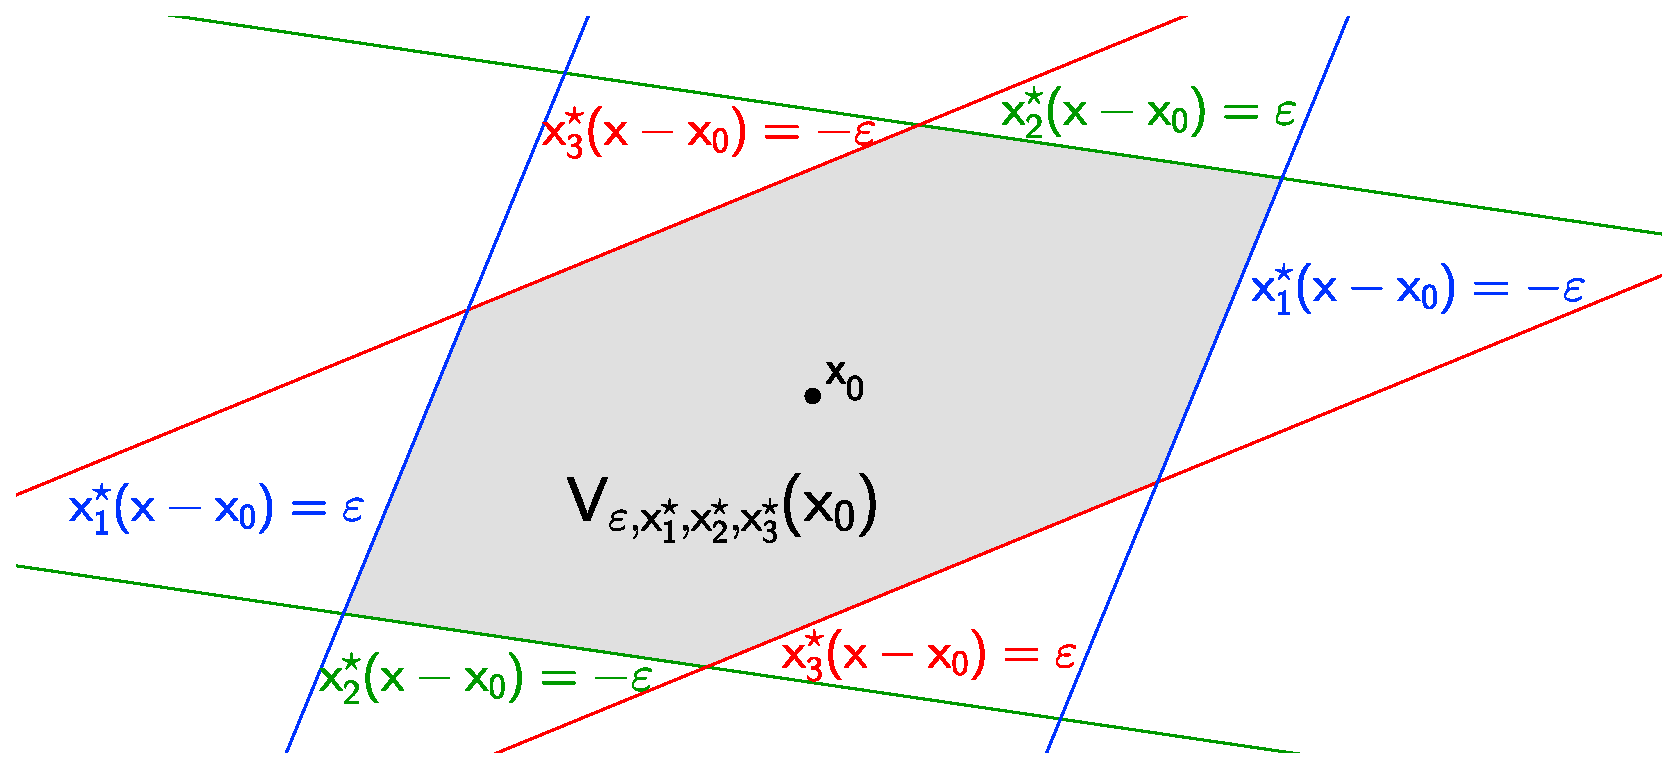
\includegraphics[width = 10.1cm,height=4.9cm]{topo/voisinagefaible.eps}}
\end{tabular}\end{center}

\section{Topologie pr�faible}

Soit $E$ un espace vectoriel norm�. Soient $x_0\dual\in E\dual, \varepsilon>0, n\in\mathbb{N}_0, x_1,...,x_n\in E$. On d�finit
\[
V_{\varepsilon, x_1,...,x_n}(x_0\dual)=
\{x\dual\in E\dual~|~\forall k\in\{1,...,n\}, \abs{(x\dual-x_0\dual)(x_k)}<\varepsilon\}
\]
Le syst�me fondamental de voisinages que l'on d�finit pour $x_0\dual$ est
\[
\{V_{\varepsilon, x_1,...,x_n}(x_0\dual)~|~\varepsilon>0, n\in\mathbb{N}_0, x_1,...,x_n\in E\}
\]
En fait, c'est m�me un syst�me fondamental de voisinages ouverts. On appliquera le m�me raisonnement que pour la topologie faible.

Cette topologie sur $E\dual$ est appel�e topologie pr�faible, et est not�e $\pweak{E}$ ou $\omega\star$.

Pour cette topologie, une suite $(x_n\dual)_{n\in\mathbb{N}}$ � valeurs dans $E\dual$ converge vers $x\dual\in E\dual$ si et seulement si pour tout $x\in E$, on a $x_n\dual(x)\rightarrow x\dual(x)$.



\section{Propri�t�s de ces topologies}

Ces deux nouvelles topologies n'ont aucun int�r�t dans le cas d'un espace vectoriel de dimension finie, car elles co�ncident avec la topologie de la norme. En revanche, nous verrons que dans le cas d'un espace de dimension infinie, il peut y avoir de nombreuses diff�rences entre ces trois topologies.

\begin{Rem}
Sur $E\dual$, la topologie $\pweak{E}$ est plus faible que la topologie $\weak{E\dual}$. En effet, tous les voisinages utilis�s pour d�finir la topologie $\pweak{E}$ sont de la forme
\begin{align*}
V_{\varepsilon, x_1,...,x_n}(x_0\dual)
&= \{x\dual\in E\dual~|~\forall k\in\{1,...,n\}, \abs{(x\dual-x_0\dual)(x_k)}<\varepsilon\} \\
&= \{x\dual\in E\dual~|~\forall k\in\{1,...,n\}, \abs{ev_{x_k}(x\dual-x_0\dual)}<\varepsilon\} \\
&= V_{\varepsilon, ev_{x_1},...,ev_{x_n}}(x_0\dual)
\end{align*}
qui sont tous des voisinages pour $\weak{E\dual}$.
\end{Rem}

\begin{Prop}\label{contiforteimpliquefaible}
Soient $E$, $F$ deux espaces vectoriels norm�s et $T:E\maps F$ une application lin�aire continue. Alors $T:(E,\weak{E}\maps(F,\weak{F})$ est continue.
\end{Prop}
\begin{proof}
Soient $x_0\in E$ et un ouvert faible contenant $T(x_0)$ de la forme $V_{\varepsilon, x_1\dual,...,x_n\dual}(T(x_0))$. Puisque $T$ est fortement continue, les applications $x\dual\circ T:E\maps\mathbb{K}$ sont fortement continues. Par cons�quent
\[
\inv{T}(V_{\varepsilon, x_1\dual,...,x_n\dual}(T(x_0))) =
\{x\in E~|~\forall k\in\{1,...,n\}, \abs{x_k\dual(T(x)-T(x_0))}<\varepsilon\} =
V_{\varepsilon, x_1\dual\circ T,...,x_n\dual\circ T}(x_0)
\]
est bien un ouvert faible de $E$.
\end{proof}

\begin{Prop}\label{topowsepare}
Les topologies $\weak{E}$ et $\pweak{E}$ sont s�par�es.
\end{Prop}
\begin{proof}
On commence par $\weak{E}$. Soient $x\neq y\in E$. Par le th�or�me de Hahn-Banach (\ref{HBF}), on a $x\dual\in E\dual$ tel que $x\dual(x-y)=\norme{x-y}>0$. Alors les voisinages de $x$ et de $y$ sont ceux d�finis par $\varepsilon=\frac{\norme{x-y}}{3}$, $n=1$ et $x_1\dual = x\dual$.
On finit par $\pweak{E}$. Soient $x\dual\neq y\dual\in E\dual$. Puisque $x\dual\neq y\dual$, il existe $x\in E$ tel que $(x\dual-y\dual)(x)>0$. On conclut en prenant $\varepsilon=\frac{(x\dual-y\dual)(x)}{3}>0$, $n=1$, $x_1=x$ pour d�finir les voisinages de $x\dual$ et de $y\dual$.\\
\end{proof}

\begin{Prop}\label{topownonborne}
Si $E$ est un espace vectoriel norm� de dimension infinie, alors aucun voisinage des topologies $\weak{E}$ et $\pweak{E}$ n'est born� pour la topologie de la norme.
\end{Prop}
\begin{proof}
Soient $\varepsilon>0,n\in\mathbb{N}_0$ et $x_1\dual,...,x_n\dual\in E\dual$. On a que $\codim(\ker(x_k\dual))\leqslant 1$, quelque soit $k\in\{1,...,n\}$. Par cons�quent, $\dim\left(\bigcap\limits_{k=1}^n \ker(x_k\dual)\right)=+\infty$, on peut donc trouver, quelque soit $\alpha>0$, $x\in E$ tel que $\norme{x}=\alpha$ et $x_k\dual(x)=0$ pour tout $k\in\{1,...,n\}$, c'est-�-dire que $x\in V_{\varepsilon, x_1\dual,...,x_n\dual}(0)$. Par un raisonnement identique, on obtient le m�me r�sultat pour la topologie pr�faible.
\end{proof}

\begin{Corol}\label{spheredenseboulevide}
Pour les topologies faible et pr�faible en dimension infinie, les sph�res sont denses dans les boules, et les boules sont d'int�rieur vide.
\end{Corol}
\begin{proof}
On le d�montre pour des boules et des sph�res centr�es en 0 et de rayon 1.

Soient $x\in B(E)$ et $V_x$ un voisinage faible de $x$. Ce voisinage n'est pas born� pour la norme, donc il contient n�cessairement un point $y\in E$ tel que $\norme{y}=1$, d'o� $V_x\cap S(E)\neq\emptyset$. Ceci implique que $\adh{S(E)}\supseteq B(E)$.

Soient $x\in E$ et $V_x$ un voisinage faible de $x$. Le voisinage n'�tant pas born� pour la norme, il n'est pas inclu dans $B(E)$, et donc $x$ n'est pas dans l'int�rieur de $B(E)$.

Pour la topologie pr�faible, tous ces arguments sont valables.
\end{proof}

\begin{Rem}
En fait, c'est un peu plus fort. On peut appliquer le m�me raisonnement � tout sous-ensemble de $B(E)$, on en d�duit que tout ensemble born� pour la norme est d'int�rieur vide pour les topologies faible et pr�faible. De plus pour la topologie faible, toutes les adh�rences de sph�res sont des boules ferm�es pour la norme. Ceci r�sulte du th�or�me suivant:
\end{Rem}

\begin{Thm}[Mazur]\label{mazur}
Soit $C\subseteq E$ un convexe. Alors
\[C\text{ est ferm� pour }\norme{.}\ssi C\text{ est ferm� pour }\weak{E}\]
\end{Thm}

\begin{Rem}Le fait de consid�rer un convexe est indispensable pour garantir l'�quivalence, puisqu'on vient de voir que la sph�re unit� est dense dans la boule unit� (voir la proposition \ref{spheredenseboulevide})). Par cons�quent, cette sph�re, bien que ferm�e pour la norme, n'est pas ferm�e pour la topologie faible.\end{Rem}

\begin{Rem}La m�me �quivalence, o� l'on remplace les ferm�s par des ouverts, n'est vraie qu'en dimension finie. Ceci est une cons�quence imm�diate du fait qu'un voisinage faible ne peut �tre born� pour la norme qu'en dimension finie (voir la proposition (\ref{topownonborne})).\end{Rem}

On est en droit de se demander si le th�or�me de Mazur vaut aussi pour la topologie pr�faible, quand celle-ci est d�finie. Le lemme suivant r�pond par la n�gative:

\begin{Lemme}[Goldstine]\label{goldstine}
Pour $\pweak{E\dual}$, $i(B(E))$ est dense dans $B(E\bidual)$.
\end{Lemme}
\begin{Rem}
Si $E$ est r�flexif, la conclusion est �vidente, puisque $i(B(E))=B(E\bidual)$. Dans le cas d'un espace non r�flexif, ce lemme fournit un bel exemple de ferm� convexe fort qui n'est pas ferm� pr�faible.
\end{Rem}
\begin{proof}
Soient $x\bidual\in B(E\bidual)$ et $V$ un voisinage de $x\bidual$. On peut supposer qu'il est de la forme $V_{\varepsilon, x_1\dual,...,x_n\dual}(x\bidual)$. On pose $\alpha=(\alpha_1,...,\alpha_n)=(x\bidual(x_1\dual),...,x\bidual(x_n\dual))$ et
\begin{align*}
\varphi&:&E&\maps&\mathbb{K}^n\\
&:&n&\mapsto&(x_1\dual(x),...,x_n\dual(x))=(ev_x(x_1\dual),...,ev_x(x_n\dual))
\end{align*}

On d�montrera deux r�sultats interm�diaires avant de conclure:
\begin{itemize}
\item $\forall\beta_1,...,\beta_n\in\mathbb{K}, \abs{\sum\limits_{k=1}^n \alpha_k\beta_k}\leqslant\norme{\sum\limits_{k=1}^n \beta_k x_k\dual}$
\item $\alpha\in\conj{\varphi(B(E))}$
\end{itemize}

Soient $\beta_1,...,\beta_n\in\mathbb{K}$. On a que
\[
\abs{\sum_{k=1}^n \alpha_k\beta_k} =
\abs{\sum_{k=1}^n \beta_k x\bidual(x_k\dual)} =
\abs{x\bidual\left(\sum_{k=1}^n \beta_k x_k\dual\right)} \leqslant
\norme{\sum_{k=1}^n \beta_k x_k\dual}
\]

Maintenant, supposons par l'absurde que $\alpha\notin\conj{\varphi(B(E))}$. Dans ce cas, par le th�or�me de Hahn-Banach (\ref{HBC}), on peut s�parer $\{\alpha\}$ et $\conj{\varphi(B(E))}$. On obtient alors $y\dual\in(\mathbb{K}^n)\dual$ et $\gamma>0$ tels que pour tout $z\in \conj{\varphi(B(E))}$, $\abs{y\dual(z)}<\gamma<\abs{y\dual(\alpha)}$. En particulier, c'est aussi vrai pour les $\varphi(x)$, o� $x\in B(E)$. Identifions $y\dual$ avec $(\beta_1,...,\beta_n)\in\mathbb{K}^n$, et prenons $x\in B(E)$. On a
\[
\begin{array}{rrrrr}
\abs{y\dual(\varphi(x))} & < & \gamma & < & \abs{y\dual(\alpha)}\\
\abs{\displaystyle\sum_{k=1}^n \beta_k x_k\dual(x)} & < & \gamma & < & \abs{\displaystyle\sum_{k=1}^n \alpha_k\beta_k}\\
\text{par passage au supremum}\\
\norme{\displaystyle\sum_{k=1}^n \beta_k x_k\dual} & \leqslant & \gamma & < & \abs{\displaystyle\sum_{k=1}^n \alpha_k\beta_k}\\
\end{array}
\]
Or, on vient de d�montrer que $\norme{\sum\limits_{k=1}^n \beta_k x_k\dual}<\abs{\sum\limits_{k=1}^n \alpha_k\beta_k}\leqslant\norme{\sum\limits_{k=1}^n \beta_k x_k\dual}$, ce qui est absurde.

On a par cons�quent que $\alpha\in\conj{\varphi(B(E))}$. Dans ce cas, il existe une suite $(x_m)_{m\in\mathbb{N}}$ � valeurs dans $B(E)$ telle que $\varphi(x_m)\rightarrow\alpha$, c'est � dire que $\norme{\varphi(x_m)-\alpha}\rightarrow 0$. Puisque dans $\mathbb{K}^n$ toutes les normes sont �quivalentes, c'est vrai aussi pour la norme infinie, on obtient donc que $\abs{x_k\dual(x_m)-x\bidual(x_k\dual)}\rightarrow 0$, quelque soit $k\in\{1,...,n\}$. On en d�duit alors qu'il existe $N\in\mathbb{N}$ tel que $\abs{ev_{x_N^{ }}(x_k\dual)-x\bidual(x_k\dual)}<\varepsilon$ quelque soit $k\in\{1,...,n\}$, et on a $ev_{x_N^{ }}\in V_{\varepsilon, x_1\dual,...,x_n\dual}(x\bidual)$, c'est-�-dire que $i(B(E))$ est dense dans $B(E\bidual)$ pour $\pweak{E\dual}$.
\end{proof}




\section{Topologie initiale}

Soient $I$ un ensemble quelconque non vide, $(Y_i)_{i\in I}$ une famille d'espaces topologiques, $X$ un ensemble et pour tout $i\in I$, une application $f_i:X\maps Y_i$.

\begin{Def}
On appelle topologie initiale (sur $X$) la topologie la plus faible qui rende continues toutes les $f_i$, pour $i\in I$.
\end{Def}

\begin{Prop}
Les topologies faible et pr�faible sont des topologies initiales.
\end{Prop}
\begin{proof}
Pour la topologie faible, prendre $X=E$, $I=E\dual$ et pour tout $x\dual\in I$, $f_{x\dual} = x\dual$ et $Y_{x\dual}=\mathbb{K}$ muni de la topologie usuelle. Pour la topologie pr�faible, prendre $X=E\dual$, $I=E$ et pour tout $x\in I$, $f_{x}=ev_x$ et $Y_{x}=\mathbb{K}$ muni de la topologie usuelle.
\end{proof}

\begin{Def}[Topologie produit]\label{topoprod}
Posons $X=\prod\limits_{i\in I}Y_i$, dans lequel un �l�ment $x\in X$ se note $(x_i)_{i\in I}$, o� $x_i\in Y_i$, pour tout $i\in I$. On d�finit, pour tout $i\in I$, les applications
\[
\begin{array}{lllll}
\pi_i&:&X&\maps&Y_i\\
&:&x&\mapsto&x_i
\end{array}
\]
appel�es projections. La topologie sur $X$ la moins fine qui rende continues toutes les projections, est appel�e topologie produit et est not�e $\Tau_\pi$.
\end{Def}

La topologie produit est clairement une topologie initiale.

\begin{Prop}\label{proptopoinit}
On munit $X$ de la topologie initiale. Soit $Z$ un espace topologique et une application $\varphi:Z\maps X$. Alors les assertions suivantes sont �quivalentes:
\begin{itemize}
\item $\varphi$ est continue
\item $\forall i\in I, \varphi\circ f_i$ est continue
\end{itemize}
\end{Prop}




    \chapter{Premi�res caract�risations de la r�flexivit�}\label{chapter_compact_geom}

\chapter{Premi�res caract�risations de la r�flexivit�}

\section{Th�or�mes de compacit�}

Tout d'abord, rappelons deux th�or�mes tr�s importants qui, pour un espace vectoriel norm� $E$, caract�risent la compacit� de la boule unit�.
\begin{Thm}[Riesz]\label{rieszboule}
$B(E)\text{ est compacte }\ssi\dim(E)<+\infty$
\end{Thm}
\begin{Thm}[Alaoglu]\label{alaoglu}
$B(E\dual)$ est compacte pour la topologie $\pweak{E}$.
\end{Thm}

\begin{Rem}
Ceci peut para�tre surprenant, voire m�me contradictoire, mais il n'en est rien. Le th�or�me de Riesz s'applique pour la topologie de la norme, alors que le th�or�me d'Alaoglu s'applique sur la topologie pr�faible, qui est strictement plus faible que la topologie de la norme en dimension infinie. Le seul cas o� la topologie de la norme co�ncide avec la topologie pr�faible, c'est en dimension finie. Dans ce cas, le dual est aussi de dimension finie, et les deux th�or�mes affirment alors que la boule unit� du dual est compacte.
\end{Rem}
Pour d�montrer le th�or�me d'Alaoglu, nous aurons besoin du th�or�me suivant:

\begin{Thm}[Tychonoff]\label{tychonoff}
Un produit quelconque d'espaces topologiques compacts est un espace topologique compact, pour la topologie produit.
\end{Thm}

\begin{proof}[D�monstration du th�or�me d'Alaoglu]
On va proc�der en deux �tapes:
\begin{itemize}
\item On cherche un hom�omorphisme $\varphi$ de $(E,\pweak{E})$ vers un espace dans lequel on connait des compacts
\item On montre que l'image de $B(E\dual)$ est incluse � un compact
\end{itemize}
En faisant cela, on aura d�montr� le th�or�me. En effet, on aura que $\varphi(B(E\dual))$ est ferm�e puisque $\varphi$ est un hom�omorphisme. On l'aura inclus � un compact, donc $\varphi(B(E\dual))$ sera compact. Et puisque $\varphi$ est un hom�omorphisme,  $\varphi(B(E\dual))$ compact $\ssi$  $B(E\dual)$ compacte.

\subsubsection*{Premi�re �tape}
On d�finit l'application lin�aire $\varphi:E\dual\maps\mathbb{K}^E:x\dual\mapsto (x\dual(x))_{x\in E}$. Cette application est clairement injective, et par cons�quent bijective sur son image. Munissons $E$ de la topologie $\pweak{E}$ et $\mathbb{K}^E$ de la topologie produit $\Tau_\pi$ (d�finition (\ref{topoprod})).

Alors $\varphi:(E\dual,\pweak{E})\maps(\varphi(E\dual),\Tau_{\pi,ind})$ est une application bicontinue.

Si $\varphi:(E,\pweak{E})\maps(\mathbb{K}^E, \Tau_\pi)$ est continue, alors elle le sera aussi sur son image. Par la proposition (\ref{proptopoinit}), $\varphi$ est continue si et seulement si toutes les $\pi_x\circ\varphi$ le sont, pour $x\in E$. Soient donc $x\in E$ et $x\dual\in E\dual$. On a que $\pi_x(\varphi(x\dual))=x\dual(x)=ev_x(x\dual)$, par cons�quent $\pi_x\circ\varphi=ev_x$ est continue.

Montrons maintenant que $\inv{\varphi}:(\varphi(E\dual),\Tau_{\pi,ind})\maps(E\dual,\pweak{E})$ est continue. Par la proposition (\ref{proptopoinit}), on montrera que pour tout $x\bidual\in i(E), x\bidual\circ\inv{\varphi}$ est continue. Soient alors $x\bidual\in i(E)$ et $\omega\in\varphi(E\dual)$. On r��crit tout de suite $\omega=\varphi(x\dual)$ pour $x\dual\in E\dual$, et $x\bidual=ev_x$ pour $x\in E$. On obtiens alors $x\bidual(\inv{\varphi}(\omega))=ev_x(x\dual)=\pi_x(\omega)$, d'o� $x\bidual\circ\inv{\varphi}=\pi_x$ est continue.

\subsubsection*{Deuxi�me �tape}
Pour trouver le compact dont on a besoin, on va utiliser le th�or�me de Tychonoff (\ref{tychonoff}). Dans $\mathbb{K}$, tout ensemble de la forme $\{a\in\mathbb{K}|\abs{a}\leqslant\lambda\}$ est compact, pour $\lambda\in\mathbb{R}$. D�s lors, l'ensemble $K=\{(\omega_x)_{x\in E}|\abs{\omega_x}\leqslant\norme{x}\}$ est un compact de $(\mathbb{K}^E,\Tau_\pi)$ et donc aussi de $(\varphi(E\dual),\Tau_{\pi,ind})$. On a bien que $\varphi(B(E\dual)) \subset K$ puisque la condition pour �tre dans $K$ est une condition de continuit� des applications lin�aires de $B(E\dual)$.
\end{proof}

Nous avons maintenant en main presque tout ce qu'il nous faut pour donner une caract�risation topologique des espaces r�flexifs. Il ne nous manque que lemme:

\begin{Prop}\label{iwbicont}
Si $E$ est r�flexif, alors $i:(E,\weak{E})\maps(E\bidual,\pweak{E\dual})$ est bicontinue.
\end{Prop}
\begin{proof}
Puisque $i$ est continue pour la norme, elle est continue pour les topologies faibles. Et comme $\pweak{E\dual}$ est plus faible que $\weak{E\bidual}$, on a la continuit� souhait�e. Passons � la continuit� de l'inverse. Pour ce faire, on va d�montrer que pour tout $x\dual\in E\dual$, $x\dual\circ\inv{i}$ est continue. Soient alors $x\dual\in E\dual$ et $x\bidual\in E\bidual$. Comme $E$ est r�flexif, il existe $x\in E$ tel que $ev_x=x\bidual$. On a
\[
x\dual(\inv{i}(x\bidual)) =
x\dual(x)=
x\bidual(x\dual)=
ev_{x\dual}(x\bidual)
\]
Ce qui veut dire que $x\dual\circ\inv{i}=ev_{x\dual}$ est continue. On conclut par la proposition (\ref{proptopoinit}).
\end{proof}

Ce th�or�me, qui donne une caract�risation topologique des espaces r�flexifs, fait suite aux th�or�mes de Riesz et d'Alaoglu.

\begin{Thm}[Kakutani]\label{kakutani}
$E$ est r�flexif $\ssi B(E)$ est compacte pour $\weak{E}$.
\end{Thm}
\begin{proof}
On consid�rera ici $i:(E,\weak{E})\maps(E\bidual,\pweak{E\dual})$.

$\Rightarrow)$ $E$ est r�flexif, donc $i$ est un hom�omorphisme, par le lemme (\ref{iwbicont}). Donc $B(E)$ est compacte pour $\weak{E}$ si et seulement si $i(B(E))$ est compacte pour $\pweak{E\dual}$. Le th�or�me d'Alaoglu (\ref{alaoglu}), appliqu� sur $E\dual$, dit que $B(E\bidual)$ est compacte pour $\pweak{E\dual}$. Mais comme $E$ est r�flexif, $i(B(E))=B(E\bidual)$, on en d�duit alors que $B(E)$ est compacte pour $\weak{E}$.

$\Leftarrow)$ $B(E)$ est compacte pour $\weak{E}$, donc comme $i$ est continue, $i(B(E))$ est compacte pour $\pweak{E\dual}$. De plus, $\conj{i(B(E))}=B(E\bidual)$ par le lemme de Goldstine (\ref{goldstine}). Mais $i(B(E))$ �tant compacte, est aussi ferm�e. On obtient alors $i(B(E))=B(E\bidual)$, autrement dit $i$ est surjectif.
\end{proof}

Gr�ce � ce th�or�me, nous pouvons donner une d�monstration consid�rablement plus courte de la propri�t� suivante:

\begin{Prop}Si un espace est r�flexif, alors tous ses sous-espaces ferm�s le sont, ainsi que son dual.\end{Prop}
\begin{proof}

Par le th�or�me d'Alaoglu (\ref{alaoglu}), $B(E\dual)$ est compacte pour $\pweak{E}$. Or $E$ est r�flexif, donc $\pweak{E}=\weak{E\dual}$, et $B(E\dual)$ est compacte pour $\weak{E\dual}$. On conclut en utilisant le th�or�me de Kakutani que $E\dual$ est r�flexif.\newline

Soit $F$ un sous-espace vectoriel ferm� de $E$. Comme $B(F)=F\cap B(E)$ est l'intersection de deux ferm�s convexes de $E$, c'est aussi un ferm� convexe de $E$. Comme $E$ est r�flexif, $B(E)$ est compacte pour $\weak{E}$ par le th�or�me de Kakutani (\ref{kakutani}). Par le th�or�me de Mazur (\ref{mazur}), $B(F)$ est ferm�e pour $\weak{E}$. Alors comme $B(F)\subseteq B(E)$, elle est compacte pour $\weak{E}$. Mais $\weak{F}$ �tant la topologie induite par $\weak{E}$ sur $F$, on obtient que $B(F)$ est compacte pour $\weak{F}$, donc par le th�or�me de Kakutani, $F$ est r�flexif.
\end{proof}

Nous aurons l'occasion d'exploiter ce th�or�me � de nombreuses reprises par la suite.


\section{Propri�t�s g�om�triques}

� l'oppos� du th�or�me de Kakutani, qui est p�rement topologique, on va d�montrer un th�or�me d� � James qui donne une caract�risation g�om�trique des espaces r�flexifs. Pour ceci, nous aurons besoin de plusieurs r�sultats interm�diaires.

\begin{Lemme}[Condition d'Helly]\label{hellycondition}
Soit $E$ un espace vectoriel norm� de dimension infinie. Soient $n\in\mathbb{N}_0$, $x\dual_1,...,x\dual_n\in E\dual$, $c_1,...,c_n\in\mathbb{K}$ et $M>0$. Alors, les assertions suivantes sont �quivalentes:
\begin{enumerate}[(1)]
\item Pour tout $\varepsilon>0$, il existe $x\in E$ tel que $\norme{x}=M+\varepsilon$ et $x\dual_k(x)=c_k$ quelque soit $k\in\{1,...,n\}$
\item Pour tout $a_1,...,a_n\in\mathbb{K}$, $\abs{\sum\limits_{k=1}^n a_k c_k} \leqslant M\norme{\sum\limits_{k=1}^n a_k x\dual_k}$
\end{enumerate}
\end{Lemme}
\begin{proof}
~

(1) $\Rightarrow$ (2)\\
%
Soient $\varepsilon>0$ et soit $x\in E$ tel que donn� par (1). Soient $a_1,...,a_n\in\mathbb{K}$. On a
\[
\abs{\sum_{k=1}^n a_k c_k}
=
\norme{\sum_{k=1}^n a_k x\dual_k(x)}
\leqslant
\norme{x}\norme{\sum_{k=1}^n a_k x\dual_k}
=
(M+\varepsilon)\norme{\sum_{k=1}^n a_k x\dual_k}
\]
D'o� on en d�duit (2).\newline

(2) $\Rightarrow$ (1)\\
%
Soit $\varepsilon>0$. Si $c_1=...=c_n=0$, alors il suffit de prendre un point de norme $M+\varepsilon$ qui annule toutes les $x\dual_k$. Puisque l'on est en dimension infinie, un tel point existe toujours. On se place dans le cas o� au moins l'un des $c_k$ est non-nul, sans perte de g�n�ralit� on consid�re que c'est $c_1$.

Supposons que $x\dual_1,...,x\dual_n$ soient lin�airement ind�pendants. Alors, on d�finit les hyperplans affins $H_k=\inv{x\dual_k}(c_k)$, pour $k\in\{1,...,n\}$, ainsi que $H=\bigcap\limits_{k=1}^n H_k$. Puisque les $H_k$ sont les translat�s d'espaces vectoriels de codimension 1 dans un espace de dimension infinie, on a que leur intersection $H$ est non vide. Posons $a=\inf\limits_{x\in H}\norme{x}$. On a que $a>0$ car quelque soit $x\in H$, $x\dual_1(x)=c_1\neq 0$. Alors, $H$ ne rencontre pas la boule ouverte centr�e en z�ro et de rayon $a$. Donc, par le th�or�me de Hahn-Banach (\ref{HBH}), il existe $x\dual\in E\dual$ et $c\in\mathbb{K}$ tels que $H\subseteq\mathcal{H}=\inv{x\dual}(c)$ et $\mathcal{H}$ ne rencontre pas la boule ouverte centr�e en z�ro et de rayon $a$.

Puisque $H\subseteq\mathcal{H}$, on a �galement que $\bigcap\limits_{k=1}^n \ker(x_k\dual)\subseteq\ker(x\dual)$, il suffit en effet de consid�rer, $x\in H$ et on a que $H_k$ est un espace vectoriel, quelque soit $k\in\{1,...,n\}$. Alors par le lemme (\ref{lemmealgebrique}), $x\dual$ est une combinaison lin�aire de $x\dual_1,...,x\dual_n$. Soient $a_1,...,a_n$ tels que $x\dual=\sum\limits_{k=1}^n a_k x\dual_k$. Pour $x\in\mathcal{H}$ quelconque, on a
\[
c
=
x\dual(x)
=
\sum\limits_{k=1}^n a_k x\dual_k(x)
=
\sum\limits_{k=1}^n a_k c_k
\]

Puisque $H\subseteq \mathcal{H}$, on a que $\inf\limits_{x\in H}\norme{x}\geqslant\inf\limits_{x\in\mathcal{H}}\norme{x}$. Or, $\mathcal{H}$ ne rencontre pas la boule centr�e en z�ro de rayon $a$, donc $\inf\limits_{x\in H}\norme{x}=a\leqslant\inf\limits_{x\in\mathcal{H}}\norme{x}$. De plus, $c\neq 0$, car sinon on aurait que $0\in\mathcal{H}$, et donc que $\mathcal{H}$ rencontre la boule centr�e en z�ro et de rayon $a$. On a alors que

\begin{align*}
\inf_{x\in H}\norme{x}
&=
\inf_{x\in\mathcal{H}}\frac{\norme{x}}{\abs{x\dual(x)}}\abs{x\dual(x)}
=
\abs{c}\inf_{x\in\mathcal{H}}\frac{\norme{x}}{\abs{x\dual(x)}} 
=
\abs{c}\frac{1}{\sup\limits_{x\in\mathcal{H}}\frac{\abs{x\dual(x)}}{\norme{x}}} \\
&=
\abs{c}\frac{1}{\norme{x\dual}} \hspace{8cm} \text{par la proposition (\ref{lipschitz})}\\
&=
\frac{\abs{\sum\limits_{k=1}^n a_k c_k}}{\norme{\sum\limits_{k=1}^n a_k x\dual_k}}
\end{align*}

Par hypoth�se, le dernier membre est inf�rieur � $M$. Donc, il existe $x\in H$ pour lequel $\norme{x}=M+\varepsilon$, ce que l'on cherchait.\newline

Maintenant, supposons que $n\geqslant 2$, que les $n-1$ premi�res fonctionnelles soient lin�airement ind�pendantes et que la derni�re soit une combinaison lin�aire des autres. Cela sera suffisant pour prouver que le lemme est vrai en toute g�n�ralit�. Alors, il existe $a_1,...,a_{n-1}\in\mathbb{K}$ tels que $x\dual_n=\sum\limits_{k=1}^{n-1}a_k x\dual_k$. Dans ce cas, par (2) on a que
\[
\abs{c_n-\sum_{k=1}^{n-1}a_k c_k}
\leqslant
M\norme{x\dual_n-\sum_{k=1}^{n-1}a_k x\dual_k}
=
0
\]
D'o� $c_n=\sum\limits_{k=1}^{n-1}a_k c_k$. On applique le lemme sur les $n-1$ premi�res fonctionnelles, on obtient $x$ tel que $\norme{x}=M+\varepsilon$ et $x\dual_k(x)=c_k$, quelque soit $k\in\{1,...,n-1\}$, o� $\varepsilon>0$. Alors
\[
x\dual_n(x)
=
\sum_{k=1}^{n-1}a_k x\dual_k(x)
=
\sum_{k=1}^{n-1}a_k c_k
=
c_n
\]
\end{proof}



\begin{Thm}[James]\label{jamesgeom}
Les assertions suivantes sont �quivalentes:
\begin{enumerate}[(1)]
\item $E$ n'est pas r�flexif
\item Quelque soit $\theta\in~]0,1[$, il existe une suite $(x_n)_{n\in\mathbb{N}}$ � valeurs dans $S(E)$ et une suite $(x\dual_n)_{n\in\mathbb{N}}$ � valeurs dans $S(E\dual)$ telles que, pour tout $n,m\in\mathbb{N}$
\[
x\dual_n(x_m) =
\begin{cases}
\theta & ~si~~~ n\leqslant m\\
0 & ~si~~~ n > m
\end{cases}
\]
\item Quelque soit $\theta\in~]0,1[$, il existe une suite $(x_n)_{n\in\mathbb{N}}$ � valeurs dans $S(E)$ telle que pour tout $k<K\in\mathbb{N}$, on a $\dist(\conv(x_1,...,x_k), \conv(x_{k+1},...,x_K))\geqslant\theta$
\end{enumerate}
\end{Thm}
\begin{Rem}
La propri�t� (3) est aussi appel�e "Condition J".
\end{Rem}
\begin{proof}
~

(1) $\Rightarrow$ (2)\\
%
Puisque $E$ n'est pas r�flexif, on sait que $i(E)$ est un sous-espace ferm� non trivial de $E\bidual$, et de dimension infinie. On peut alors trouver une fonctionnelle $x\tridual$ de norme 1 qui s'annule sur $i(E)$. Soient $\theta\in~]0,1[$ et $x\bidual\in E\bidual$ tels que $\norme{x\bidual}<1$ et $x\tridual(x\bidual)>\theta$. On a que $\norme{x\bidual}>\theta$. On va construire par induction les deux suites qui correspondent � ce que l'on cherche, v�rifiant en plus que $x\bidual(x\dual_n)=\theta$, pour tout $n\in\mathbb{N}$.\newline

La premi�re �tape de l'induction consiste � choisir $x_0$ et $x\dual_0$. Puisque $\norme{x\bidual}>\theta$, il existe $x\dual_0\in S(E\dual)$ tel que $x\bidual(x\dual_0)=\theta$. On trouve de mani�re semblable $x_0\in S(E)$ tel que $x\dual_0(x_0)=\theta$.\newline

Maintenant, supposons que l'on ait $x_0,...,x_n$, $x\dual_0,...,x\dual_n$ qui satisfont aux conditions d'induction. On choisit $x\dual_{n+1}\in S(E\dual)$ qui s'annule en chaque $x_k$, tel que $x\bidual(x\dual_{n+1})=\theta$, en appliquant la condition d'Helly (\ref{hellycondition}) sur $E\dual$, avec les fonctionnelles $ev_{x_0},...,ev_{x_n}, x\bidual$, associ�es aux scalaires $0,...,0,\theta$, et $M=\frac{\theta}{x\tridual(x\bidual)}<1$. Ce choix est possible puisque pour tout $a,a_0,...,a_n\in\mathbb{K}$, on a

\[
\begin{array}{ll}
\abs{a\theta}
&
\displaystyle
=
\frac{\theta}{x\tridual(x\bidual)}x\tridual(x\bidual)\abs{a}
=
M\abs{x\tridual(a x\bidual)}
=
M\abs{x\tridual\left(a x\bidual + \sum_{k=0}^n a_k ev_{x_k}\right)}
\\
&
\displaystyle
\leqslant
M\norme{a x\bidual + \sum_{k=0}^n a_k ev_{x_k}}
\end{array}
\]

� nouveau, pour trouver $x_{n+1}$ qui satisfait aux conditions de l'induction, on applique la condition d'Helly sur $E$, en prenant les fonctionnelles $x\dual_0,...,x\dual_{n+1}$ associ�es au scalaire $\theta$, et $M=\norme{x\bidual}<1$. En effet on a, pour tout $a_0,...,a_{n+1}\in\mathbb{K}$, que
\[
\abs{\sum_{k=0}^{n+1}a_k\theta}
=
\abs{\sum_{k=0}^{n+1}a_k x\bidual(x\dual_k)}
\leqslant
\norme{x\bidual}\norme{\sum_{k=0}^{n+1}a_k x\dual_k}
=
M\norme{\sum_{k=0}^{n+1}a_k x\dual_k}
\]

Ceci termine la premi�re implication.\newline

(2) $\Rightarrow$ (3)\\
%
Soit $\theta\in~]0,1[$, par (2) on a une suite $(x_n)_{n\in\mathbb{N}}$ � valeurs dans $S(E)$ et une suite $(x\dual_n)_{n\in\mathbb{N}}$ � valeurs dans $S(E\dual)$. Soient $k\leqslant K\in\mathbb{N}$ et $a_0,...,a_K\in\mathbb{R}^+$ tels que $\sum\limits_{l=0}^k a_l=\sum\limits_{l=k+1}^K a_l=1$. Alors
\[
\theta
=
x\dual_k\left(\sum\limits_{l=k+1}^K a_l x_l-\sum\limits_{l=0}^k a_l x_l\right)
\leqslant
\norme{x\dual_k}\norme{\sum\limits_{l=k+1}^K a_l x_l-\sum\limits_{l=0}^k a_l x_l}
=
\norme{\sum\limits_{l=k+1}^K a_l x_l-\sum\limits_{l=0}^k a_l x_l}
\]

(3) $\Rightarrow$ (1)\\
%
On proc�de par contraposition. Supposons que $E$ est r�flexif. Soient $\theta\in~]0,1[$ et une suite $(x_n)_{n\in\mathbb{N}}$ � valeurs dans $S(E)$. Posons $C_k=\convAdh(x_k,x_{k+1},...)\neq\emptyset$, pour $k\in\mathbb{N}$. Il est �vident que quelque soit $k\in\mathbb{N}$, $C_k\supseteq C_{k+1}$. Les $C_k$ sont des convexes ferm�s pour la norme, donc le th�or�me de Mazur (\ref{mazur}) nous dit qu'ils sont �galement faiblement ferm�s. Par le th�or�me de Kakutani (\ref{kakutani}), puisque $E$ est r�flexif, la boule unit� est faiblement compacte, donc les $C_k$ �tant tous born�s, ils sont aussi faiblement compacts. Puisque les $C_k$ sont des compacts embo�t�s, on a que $\bigcap\limits_{k\in\mathbb{N}}C_k\neq\emptyset$.

Soit $u$ un �l�ment de cet ensemble. On a que $u\in C_0$, donc il existe $n\in\mathbb{N}$ et des scalaires $u_0,...,u_n\in\mathbb{R}^+$ tels que $\sum\limits_{k=0}^n u_k = 1$ et $\norme{u-\sum\limits_{k=0}^n u_k x_k}\leqslant\frac{\theta}{3}$. De plus, $u\in C_{n+1}$, donc il existe $N\in\mathbb{N}$ et des scalaires $u_{n+1},...,u_N\in\mathbb{R}^+$ tels que $\sum\limits_{k=n+1}^N u_k = 1$ et $\norme{u-\sum\limits_{k=n+1}^N u_k x_k}\leqslant\frac{\theta}{3}$. Par cons�quent
\[
\norme{\sum\limits_{k=0}^n u_k x_k-\sum\limits_{k=n+1}^N u_k x_k}
\leqslant
\norme{\sum\limits_{k=0}^n u_k x_k-u}+\norme{\sum\limits_{k=n+1}^N u_k x_k-u}
\leqslant
\frac{2\theta}{3}
\]
Ce qui montre que (3) est faux.
\end{proof}

\begin{Rem}
Dans la derni�re implication, on a montr� que si $E$ est r�flexif, alors quelque soit $\theta\in~]0,1[$, la propri�t� (3) est fausse. De plus, la d�monstration de l'implication (2) $\Rightarrow$ (3) dit que si on a (2) pour un $\theta$ fix�, alors on a (3) pour ce m�me $\theta$.
\end{Rem}
On obtient donc:

\begin{Corol}\label{jamesgeomexists}
Les assertions suivantes sont �quivalentes:
\begin{itemize}
\item $E$ n'est pas r�flexif
\item Il existe $\theta\in~]0,1[$ et deux suites $(x_n)_{n\in\mathbb{N}}$ � valeurs dans $S(E)$ et $(x\dual_n)_{n\in\mathbb{N}}$ � valeurs dans $S(E\dual)$ tels que, pour tout $n,m\in\mathbb{N}$
\[
x\dual_n(x_m) =
\begin{cases}
\theta & ~si~~~ n\leqslant m\\
0 & ~si~~~ n > m
\end{cases}
\]
\item Il existe $\theta\in~]0,1[$ et une suite $(x_n)_{n\in\mathbb{N}}$ � valeurs dans $S(E)$ tels que pour tout $k<K\in\mathbb{N}$, \[\dist(\conv(x_1,...,x_k), \conv(x_{k+1},...,x_K))\geqslant\theta\]
\end{itemize}
\end{Corol}

\begin{Corol}
Si toutes les suites born�es d'un espace de Banach admettent une sous-suite faiblement convergente, alors il est r�flexif.
\end{Corol}

\begin{Rem}
Ce corollaire est quelque peu suprenant, sachant qu'il donne une seule implication, alors qu'il est issu d'un th�or�me qui donne une �quivalence. Mais c'est tout-�-fait normal, car le th�or�me ne caract�rise qu'un seul type de suite born�e, et ne dit rien du tout � propos des autres suites. Cependant, le th�or�me suivant nous permet d'�tablir l'autre implication.
\end{Rem}

\begin{Thm}[Eberlein-\v{S}mulian]\label{eberlein}
Soit $A$ un sous-ensemble de $E$. Alors, pour la topologie faible, $\adh{A}$ est compact si et seulement si toute suite d'�l�ments de $A$ admet une sous-suite qui converge vers un �l�ment de $\adh{A}$.
\end{Thm}

Pour une d�monstration de ce th�or�me, voir \cite[p. 430-433]{EBERLEINSMULIAN}.

\begin{Rem}
Cela signifie que pour la topologie faible, compacit� et compacit� s�quentielle sont �quivalentes pour les ferm�s. En particulier, ceci et le th�or�me de Kakutani (\ref{kakutani}) nous indiquent que la boule unit� est s�quentiellement compacte pour la topologie faible, si et seulement si l'espace est r�flexif.
\end{Rem}




\chapterref 

La totalit� des r�sultats �nonc�s viennent du livre de Bernard Beauzamy \cite{BEAUZAMY}, mais on trouvera des diff�rences dans leurs d�monstrations. C'est le cas du th�or�me d'Alaoglu dont la d�monstration est inspir�e du livre de Ha�m Br�zis, \cite[p. 42-43]{BEAUZAMY}.

    \chapter{Bases de Schauder}\label{chapter_schauder}

Dans le chapitre pr�c�dent, on a vu une propri�t� dont la d�monstration n�cessitait le raisonnement suivant:\newline

\begin{itemize}
\item On se fixe une base alg�brique de l'espace vectoriel $E$.
\item On prend un point de $E$ et une suite qui converge vers ce point.
\item On d�compose chaque vecteur choisi suivant la base fix�e.
\item Puisque la suite est convergente, les coordonn�es sont elles aussi convergentes.\newline
\end{itemize}
Bien que ce type de raisonnement soit toujours vrai en dimension finie, ce n'est plus le cas en dimension infinie. Par exemple, pla�ons-nous dans $l^\infty$. Les $(e_n)_{n\in\mathbb{N}}$ forment une famille libre de vecteurs de $l^\infty$, mais ne forment pas une base alg�brique. La suite $x=\left(\frac{1}{n}\right)_{n\in\mathbb{N}_0}$ est lin�airement ind�pendante des $(e_n)_{n\in\mathbb{N}}$ pour des combinaisons lin�aires finies. Alors, on peut utiliser le th�or�me de la base incompl�te afin d'obtenir une base alg�brique de $l^\infty$ qui contient les $(e_n)_{n\in\mathbb{N}}$ ainsi que $x$. On consid�re maintenant la suite $(x^{(n)})_{n\in\mathbb{N}}$ telle que pour $n\in\mathbb{N}_0$, on a

\[
x^{(n)}
=
\sum_{m=1}^n \frac{e_m}{m}
\]

Que l'on peut repr�senter

\[
\begin{array}{ccccccccccccccccccc}
x^{(1)} & = & ( & 1 & , & 0 & , & 0 & & ... & & ... & & 0 & , & 0 & & ... & )\\
x^{(2)} & = & ( & 1 & , & 1/2 & , & 0 & & ... & & ... & & 0 & , & 0 & & ... & )\\
x^{(3)} & = & ( & 1 & , & 1/2 & , & 1/3 & & ... & & ... & & 0 & , & 0 & & ... & )\\
\vdots &  &  & \vdots &  & \vdots &  & \vdots &  & \ddots &  &  &  & \vdots &  & \vdots & & & \\
\vdots &  &  & \vdots &  & \vdots &  & \vdots &  &  &  & \ddots &  & \vdots &  & \vdots & & & \\
x^{(n)} & = & ( & 1 & , & 1/2 & , & 1/3 & & ... & & ... & , & 1/n & , & 0 & , & ... & )\\
\vdots &  &  & \vdots &  & \vdots &  & \vdots &  &  &  &  &  & \vdots &  & \vdots & & & \\
\end{array}
\]

On a bien que chaque $x^{(n)}$ appartient � $l^\infty$ et que $x^{(n)}\rightarrow x$. Cependant on n'a pas de convergence en coordonn�es de la base alg�brique choisie. En effet, $x$ est sa propre d�composition dans la base choisie, et quel que soit $n$, la d�composition de $x^{(n)}$ ne fait pas intervenir $x$.\newline

On va donc d�finir un nouveau type de base pour lequel la convergence g�n�rale donne la convergence des coordonn�es. Ensuite, nous �tudierons ses liens avec le dual et le bidual.

\section{Suite basique, base de Schauder, constante de base}

\begin{Def}
Soient $E$ un espace vectoriel norm� et $(e_n)_{n\in\mathbb{N}}$ une suite de vecteurs de $E$. On dira que $(e_n)_{n\in\mathbb{N}}$ est une suite basique si pour tout $x\in\SpanAdh((e_n)_{n\in\mathbb{N}})$, il existe une unique suite de scalaires $(x_n)_{n\in\mathbb{N}}$ telle que
\[\sum_{n\in\mathbb{N}}x_n e_n=x\]

Si de plus, $\SpanAdh((e_n)_{n\in\mathbb{N}})=E$, on dit que c'est une base de Schauder, et on appelle $x_n$ la $n^\text{i�me}$ coordonn�e de $x$.
\end{Def}

\subsubsection*{Exemples}
\begin{itemize}
\item La base canonique $(e_n)_{n\in\mathbb{N}}$ est une base de Schauder des espaces $c_0$ et $l^p$, pour $p\in[1,+\infty[$.
\item L'espace $l^\infty$ n'�tant pas s�parable, il ne contient aucune base de Schauder. Pour rappel, un espace vectoriel norm� est s�parable s'il admet une partie d�nombrable dense.
\end{itemize}

\begin{Lemme}\label{espseriescgebanach}
Soit $E$ un espace de Banach qui contient une suite basique $(e_n)_{n\in\mathbb{N}}$. L'espace vectoriel
\[
F =
\left\{
(a_n)_{n\in\mathbb{N}}\in\mathbb{K}^\mathbb{N}
~|~
\sum_{n\in\mathbb{N}}a_n e_n\text{ converge}
\right\},
\]
muni de la norme
\[
\norme{(a_n)_{n\in\mathbb{N}}}_F
=
\sup_{N\in\mathbb{N}}\norme{\sum_{n=0}^N a_n e_n}
\]
est un espace de Banach. De plus, l'application
\[
\begin{array}{lllll}
T&:&F&\maps&\SpanAdh((e_n)_{n\in\mathbb{N}})\\
&:&(a_n)_{n\in\mathbb{N}}&\mapsto&\displaystyle\sum_{n\in\mathbb{N}}a_n e_n
\end{array}
\]
est un isomorphisme.
\end{Lemme}
\begin{proof}
Le fait que $(F,\norme{.}_F)$ soit un espace vectoriel norm� est �vident. On montre qu'il est complet. Soit une suite de Cauchy $(a^{(n)})_{n\in\mathbb{N}}$ de vecteurs de $F$. On a que
\[
\forall\varepsilon>0,\exists n_0\in\mathbb{N}\text{ tel que }\forall n\geqslant m\geqslant n_0,
\norme{a^{(n)}-a^{(m)}}_F=\sup_{N\in\mathbb{N}}\norme{\sum_{k=0}^N (a^{(n)}_k-a^{(m)}_k)e_k}<\varepsilon
\]
d'o�
\[
\forall N\in\mathbb{N},\forall\varepsilon>0,\exists n_0\in\mathbb{N}\text{ tel que }\forall n\geqslant m\geqslant n_0,
\norme{\sum_{k=0}^N (a^{(n)}_k-a^{(m)}_k)e_k}<\varepsilon
\]
Cela signifie que pour tout $N\in\mathbb{N}$, la suite $\left(\sum\limits_{k=0}^N a^{(n)}_k e_k\right)_{n\in\mathbb{N}}$ est de Cauchy. Elle converge donc vers un �l�ment, que l'on note $y^{(N)}$. Puisque $y^{(N)}$ est une limite de combinaisons lin�aires de $e_0,...,e_N$, il existe $y^{(N)}_0,...,y^{(N)}_N\in\mathbb{K}$ tels que $y^{(N)}=\sum\limits_{k=0}^N y^{(N)}_k e_k$. De plus, $(e_n)_{n\in\mathbb{N}}$ est une suite basique de $E$, donc on peut identifier
\[
\sum_{k=0}^N \lambda_k e_k \longleftrightarrow (\lambda_0,...,\lambda_N)
\]
D'o� $(a^{(n)}_0,...,a^{(n)}_N)\underset{n\rightarrow+\infty}{\longrightarrow}(y^{(N)}_0,...,y^{(N)}_N)$, c'est-�-dire que pour $k\in\{1,...,N\}$, $(a^{(n)}_k)_{n\in\mathbb{N}}$ est convergente. On note alors $a_k$ sa limite. Puisque ce raisonnement est valable quelque soit $N$, on obtient une suite $a=(a_k)_{k\in\mathbb{N}}$. Il nous reste � d�montrer que $a\in F$ et que $a^{(n)}\rightarrow a$.

Comme $(a^{(n)})_{n\in\mathbb{N}}$ est de Cauchy, on sait que
\[
\forall\varepsilon>0,\exists n_0\in\mathbb{N}\text{ tel que }\forall n\geqslant m\geqslant n_0,\forall N\in\mathbb{N},
\norme{\sum_{k=0}^N (a^{(n)}_k-a^{(m)}_k)e_k}<\varepsilon
\]
Par passage � la limite sur $m$, on obtient
\[
\forall\varepsilon>0,\exists n_0\in\mathbb{N}\text{ tel que }\forall n\geqslant n_0,\forall N\in\mathbb{N},
\norme{\sum_{k=0}^N (a^{(n)}_k-a_k)e_k}<\varepsilon
\]
On en d�duit les deux assertions qu'il restait � prouver pour que $F$ soit un espace de Banach.

La surjectivit� de $T$ est �vidente, et l'injectivit� vient du fait que la suite $(e_n)_{n\in\mathbb{N}}$ est une suite basique. De plus, cette application est continue
\[
\norme{\sum_{n\in\mathbb{N}}a_n e_n}\leqslant \sup_{N\in\mathbb{N}}\norme{\sum_{n=0}^N a_n e_n}=\norme{(a_n)_{n\in\mathbb{N}}}_F
\]
On conclut en utilisant le th�or�me des isomorphismes de Banach.
\end{proof}

On va maintenant donner une nouvelle caract�risation aux suites basiques.

\begin{Def}
On dira qu'une suite $(e_n)_{n\in\mathbb{N}}$ de vecteurs non nuls admet une constante de base s'il existe un r�el $K>0$ tel que pour tout $p\leqslant q\in\mathbb{N}$ et $a_0,...,a_q\in\mathbb{K}$, on a
\[
\norme{\sum_{n=0}^p a_n e_n}\leqslant K\norme{\sum_{n=0}^q a_n e_n}
\]
On appellera la constante de base de $(e_n)_{n\in\mathbb{N}}$ la plus petite valeur qui v�rifie cette propri�t�. \\
Une suite basique dont la constante de base vaut 1 est appel�e suite basique monotone.
\end{Def}

\begin{Rem}
Autrement dit, dans le cas d'une suite basique et pour $p\leqslant q\in\mathbb{N}$, les projections
\[
P_{q, p}:\Span(e_0,...,e_q)\maps\Span(e_0,...,e_p)
\]
sont continues et de norme uniform�ment born�e.

Ceci implique que les projections $P_n:\SpanAdh((e_n)_{n\in\mathbb{N}})\maps\Span(e_0,...,e_n)$ sont continues et de norme uniform�ment born�e.
De plus, on se rend facilement compte en prenant $p=q$, qu'une constante de base ne peut �tre inf�rieure � 1.
\end{Rem}

\begin{Prop}\label{schauderbasique}
Dans un espace de Banach, une suite est basique si et seulement si elle admet une constante de base.
\end{Prop}
\begin{proof}
~

$\Rightarrow)$\\
%
Le lemme (\ref{espseriescgebanach}) donne la premi�re implication.

$\Leftarrow)$\\
%
Dans cette d�monstration, nous ferons appel aux notations des projections afin de simplifier l'�criture, mais n'oublions pas que cela ne repr�sente, � priori, pas une application.

Supposons que la suite admet $K>0$ comme constante de base. Soit $x\in\SpanAdh((e_n)_{n\in\mathbb{N}})$. On a une suite $(x^{(n)})_{n\in\mathbb{N}}$ de vecteurs de $\Span((e_n)_{n\in\mathbb{N}})$ qui converge vers $x$. Pour $n\in\mathbb{N}$, on r��crit
\[
x^{(n)}=\sum_{k=0}^{m_n}x^{(n)}_k e_k\text{, avec }m_n\in\mathbb{N}\text{, et pour }k\in\{0,...,m_n\}, x^{(n)}_k\in\mathbb{K}
\]
Cette suite �tant convergente, quelque soit $k\in\mathbb{N}$, la suite $\left(P_k(x^{(n)})\right)_{n\in\mathbb{N}}$ est aussi convergente, et converge vers un�l�ment que l'on note $P_k(x)$.\\
Si $k=0$, $P_0(x^{(n)})=x^{(n)}_0 e_0\rightarrow x_0 e_0$ pour un scalaire $x_0$.\\
Si $k=1$, $P_1(x^{(n)})=x^{(n)}_0 e_0+x^{(n)}_1 e_1\rightarrow x_0 e_0+x_1 e_1$ pour un scalaire $x_1$.\\
...\\
Si $k=N$, $P_N(x^{(n)})=\sum\limits_{l=0}^N x^{(n)}_l e_l\rightarrow \sum\limits_{l=0}^N x_l e_l$ pour un scalaire $x_N$.\\
...

On obtient ainsi une suite $(x_n)_{n\in\mathbb{N}}$ telle que pour tout $n\in\mathbb{N}$,
\[
P_k(x)=\sum_{l=0}^k x_l e_l
\]
Montrons que $P_k(x)\rightarrow x$. Soit $\varepsilon>0$. Puisque $x^{(n)}\rightarrow x$, il existe $n\in\mathbb{N}$ tel que $\norme{x^{(n)}-x}<\varepsilon$. Prenons $k_0 = m_{n}$. Alors, quelque soit $k\geqslant k_0$, on a que $P_k(x^{(n)})=x^{(n)}$, d'o�
\[
\begin{array}{ll}
\norme{P_k(x)-x}
&\leqslant
\norme{P_k(x)-P_k(x^{(n)})}+
\norme{P_k(x^{(n)})-x^{(n)}}+
\norme{x^{(n)}-x}
\\&\leqslant
K\norme{x^{(n)}-x}+
\norme{x^{(n)}-x}
\leqslant
(1+K)\varepsilon
\end{array}
\]
Montrons que cette d�composition est unique. Prenons une deuxi�me suite de scalaires $(y_n)_{n\in\mathbb{N}}$ telle que $\sum\limits_{n\in\mathbb{N}}y_n e_n = x$. Alors, $\sum\limits_{n\in\mathbb{N}}(x_n-y_n)e_n = 0$, donc pour tout $N\in\mathbb{N}$,
\[
\sum_{n=0}^N(x_n-y_n)e_n
=
P_N\left(\sum_{n\in\mathbb{N}}(x_n-y_n)e_n\right)
=
P_N(0)
=
0
\]
On en d�duit alors, puisque les $(e_n)_{n\in\mathbb{N}}$ sont non nuls, que les d�compositions sont �gales et donc qu'il n'y en a qu'une. Ceci termine la d�monstration.
\end{proof}

Soit $E$ un espace de Banach qui contient $(e_n)_{n\in\mathbb{N}}$ une suite basique de $E$. Au regard de la propri�t� que l'on vient de d�montrer, on d�finit les applications lin�aires
\[
\begin{array}{lllll}
f_n&:&\SpanAdh((e_n)_{n\in\mathbb{N}})&\maps&\mathbb{K}\\
&:&\displaystyle x=\sum_{n\in\mathbb{N}}x_n e_n&\mapsto&x_n
\end{array}
\]
Ces applications sont continues, car
\[
\abs{f_0(x)}=\abs{x_0}
=
\frac{\norme{x_0 e_0}}{\norme{e_0}}
=
\frac{\norme{P_0(x)}}{\norme{e_0}}
\leqslant
\frac{K}{\norme{e_0}}\norme{x}
\]
et
\[
\abs{f_{n+1}(x)}=\frac{\norme{x_{n+1} e_{n+1}}}{\norme{e_{n+1}}}
=
\frac{\norme{P_{n+1}(x)-P_n(x)}}{\norme{e_{n+1}}}
\leqslant
\frac{2K}{\norme{e_{n+1}}}\norme{x}
\]
Par cons�quent, elles peuvent �tre �tendues � $E$ par le th�or�me de Hahn-Banach (\ref{HBA}). Ces applications sont appel�es fonctionnelles coordonn�es si la suite $(e_n)_{n\in\mathbb{N}}$ est une base de Schauder. On obtient ce que l'on voulait, � savoir que pour une suite $(x_n)_{n\in\mathbb{N}}$ convergeant vers $x$, on a $f_k(x_n)\underset{n\rightarrow+\infty}{\longrightarrow} f_k(x)$ quelque soit $k\in\mathbb{N}$. Pour la m�me raison, quelque soit $x\in\SpanAdh((e_n)_{n\in\mathbb{N}})$, on a que $P_n(x)\rightarrow x$. Autrement dit, la suite des projections $(P_n)_{n\in\mathbb{N}}$ converge pr�faiblement vers l'identit� sur $\SpanAdh((e_n)_{n\in\mathbb{N}})$.

Dans le cas o� $(e_n)_{n\in\mathbb{N}}$ est une base de Schauder, on a �galement pour un vecteur $x$, l'�criture suivante:
\[
x=\sum_{n\in\mathbb{N}}f_n(x)e_n.
\]





On sait qu'un espace non s�parable ne contient aucune base de Schauder. D'ailleurs, �tre s�parable n'est pas suffisant pour forcer l'espace � contenir une base de Schauder. En effet, pour $p>1$, $p\neq 2$, l'espace $L^p([0,1])$ contient un sous-espace sans base de Schauder (voir \cite[p. 309-317]{PENFLO}). On va voir que pour les suites basiques, cela se passe diff�remment.

\begin{Lemme}\label{basiquexiste}
Soit $E$ un espace de Banach de dimension infinie contenant $(e_0,...,e_n)$ une suite finie de constante de base $K$. Quel que soit $\varepsilon>0$, on peut trouver $e_{n+1}\in S(E)$ tel que $(e_0,...,e_{n+1})$ a une constante de base inf�rieure � $K(1+\varepsilon)$.
\end{Lemme}
\begin{proof}
Soit $\varepsilon>0$, on pose $\delta=\frac{\varepsilon}{1+\varepsilon}$. Dans $\Span(e_0,...,e_n)$ la sph�re unit� est compacte, on a donc $(p_1,...,p_N)$ un $\delta$-r�seau de cette sph�re. Par le th�or�me de Hahn-Banach (\ref{HBF}), il existe $\varphi_k\in E\dual$ de norme 1 tel que $\varphi_k(p_k)=1$, quelque soit $k\in\{1,...,N\}$. Comme $E$ est de dimension infinie, il existe $e_{n+1}\in E$ tel que $\norme{e_{n+1}}=1$ et $\varphi_k(e_{n+1})=0$, quelque soit $k\in\{1,...,N\}$.

Soient $a_0,...,a_{n+1}\in\mathbb{K}$ tels que $\norme{\sum\limits_{k=0}^n a_k e_k}=1$. Il existe $m\in\{1,...,N\}$ v�rifiant
\[
\norme{p_m-\sum_{k=0}^n a_k e_k}
\leqslant \delta
\]
Alors
\begin{align*}
1 &\displaystyle
= \varphi_m\left(p_m+a_{n+1}e_{n+1}\right)
\leqslant
\norme{p_m+a_{n+1}e_{n+1}}
=
\norme{p_m+\sum_{k=0}^{n+1}a_k e_k-\sum_{k=0}^n a_k e_k}
\\&\displaystyle
\leqslant
\norme{p_m-\sum_{k=0}^n a_k e_k}+\norme{\sum_{k=0}^{n+1}a_k e_k}
\leqslant
\delta+\norme{\sum_{k=0}^{n+1}a_k e_k}
\end{align*}
D'o�
\[
\norme{\sum_{k=0}^{n+1}a_k e_k}
\geqslant
1-\delta
=
\frac{1}{1+\varepsilon}
\]
Par cons�quent
\[
(1+\varepsilon)\norme{\sum_{k=0}^{n+1}a_k e_k}
\geqslant
1 = \norme{\sum_{k=0}^{n}a_k e_k}
\]
Par homog�n��t�, le r�sultat s'�tend � toute suite finie de $n+1$ scalaires quelconques. Montrons maintenant que la suite finie $(e_0,...,e_{n+1})$ poss�de une constante de base inf�rieure � $K(1+\varepsilon)$. Les autres cas �tant �vidents, on consid�re uniquement le cas o� $p\leqslant n$ et $q=n+1$. Alors, pour $a_0,...,a_{n+1}\in\mathbb{K}$, on a
\[
\norme{\sum_{k=0}^p a_k e_k}
\leqslant
K\norme{\sum_{k=0}^n a_k e_k}
\leqslant
K(1+\varepsilon)\norme{\sum_{k=0}^{n+1} a_k e_k}
\]
\end{proof}
\begin{Corol}
Tout espace de Banach de dimension infinie admet une suite basique normalis�e. De plus, quelque soit $\varepsilon>0$, on peut choisir cette suite de telle sorte que sa constante de base soit inf�rieure � $1+\varepsilon$.
\end{Corol}
\begin{proof}
Soient $e_1\in S(E)$ et $\varepsilon>0$. Ce vecteur repr�sente une suite finie � un �l�ment de $S(E)$, de constante de base �gale � 1. On proc�de par induction sur le lemme (\ref{basiquexiste}), en choisissant $\varepsilon_n=\exp(\frac{1}{2^n}\frac{\ln(1+\varepsilon)}{2})-1>0$. � la $n^\text{i�me}$ �tape, la suite finie a une constante de base inf�rieure �

\[
\begin{array}{ll}
\displaystyle\prod_{k=0}^n(1+\varepsilon_k)
\hspace*{-0.3cm}\linebreak[0]
&\displaystyle=
\prod_{k=0}^n\exp\left(\frac{1}{2^k}\frac{\ln(1+\varepsilon)}{2}\right)
=
\exp\left(\sum_{k=0}^n\frac{1}{2^k}\frac{\ln(1+\varepsilon)}{2}\right)
\\&=
\exp\left(\left(2-\frac{1}{2^n}\right)\frac{\ln(1+\varepsilon)}{2}\right)
=
\exp\left(\ln(1+\varepsilon)-\frac{1}{2^n}\frac{\ln(1+\varepsilon)}{2}\right)
=
(1+\varepsilon)\exp\left(-\frac{1}{2^n}\frac{\ln(1+\varepsilon)}{2}\right)
\end{array}
\]

qui converge de mani�re croissante vers $1+\varepsilon$. Le lemme donne � chaque �tape un vecteur de norme 1, le corollaire est prouv�.
\end{proof}

\begin{Rem}
Avec le lemme (\ref{basiquexiste}), on ne peut pas faire mieux que le r�sultat que l'on vient de d�montrer. En effet, � partir du moment o� on a choisi le premier vecteur, la constante de base associ�e est �gale � 1. Ensuite, quelque soit $\varepsilon>0$ utilis�, le lemme ne garantit pas que la constante de base reste �gale � 1. L'existence d'une suite basique monotone est par cons�quent impossible � �tablir de cette mani�re.
\end{Rem}



\section{Base contractante, base compl�te, caract�risations du bidual}

\begin{Def}
Soit $E$ un espace de Banach contenant une base de Schauder $(e_n)_{n\in\mathbb{N}}$.\\
On dit que cette base est compl�te (boundedly-complete) si toute suite de scalaires $(a_n)_{n\in\mathbb{N}}$ telle que $\sup\limits_{N\in\mathbb{N}}\norme{\sum\limits_{n=0}^N a_n e_n}<+\infty$ rend la s�rie $\sum\limits_{n\in\mathbb{N}} a_n e_n$ convergente.\\
On dit que cette base est contractante (shrinking) si quelque soit $x\dual\in E\dual$,
\[
\sup\left\{
\abs{x\dual(x)}
\left|
\norme{x}=1\text{ et }
x=\sum_{j\geqslant n}x_j e_j,\text{ pour }(a_j)_{j\geqslant n}\in\mathbb{K}^\mathbb{N}
\right.
\right\}
\underset{n\rightarrow+\infty}{\longrightarrow}0.
\]
\end{Def}
\begin{Rem}
La d�finition d'une base contractante peut s'�crire de mani�re plus concise:
\[
\forall x\dual\in E\dual,
\sup\left\{
\abs{x\dual(x)}
\text{ tel que }
\norme{x}=1\text{ et }P_n(x)=0
\right\}
\underset{n\rightarrow+\infty}{\longrightarrow}0.
\]
\end{Rem}

\subsection*{Exemples}
\subsubsection*{Base de Schauder contractante, non compl�te}
On prend la base canonique dans $c_0$. Elle est contractante, et n'est pas compl�te. Pour d�montrer la premi�re assertion, on proc�de par l'absurde.

Supposons que la base ne soit pas contractante. Il existe alors $x\dual\in l^1$ et $\varepsilon>0$ tels que pour tout $n\in\mathbb{N}$, on trouve $N\geqslant n$ v�rifiant
\[
\sup\left\{
\abs{x\dual(x)}
\left|
\norme{x}=1\text{ et }
x=\sum_{j\geqslant N}x_j e_j,\text{ pour }(a_j)_{j\geqslant N}\in\mathbb{K}^\mathbb{N}
\right.
\right\}
>\varepsilon
\]
Puisque $x\dual\in l^1$, $x\dual=(x\dual_n)_{n\in\mathbb{N}}$ et il existe $n_0\in\mathbb{N}$ tel que $\sum\limits_{n\geqslant n_0}\abs{x\dual_n}<\varepsilon$.

Puisque la base n'est pas contractante, il existe $N\geqslant n_0$ et $x\in S(c_0)$ tel que $x=\sum\limits_{n\geqslant N}x_n e_n$ et $\abs{x\dual(x)}>\varepsilon$. Cependant,
\[
\abs{x\dual(x)}
=
\abs{\sum_{n\geqslant N}x\dual_n x_n}
\leqslant
\sum_{n\geqslant N}\abs{x\dual_n}
\leqslant
\varepsilon
\]
Ce qui est absurde.

Montrons qu'elle n'est pas compl�te. Prenons comme suite de scalaires la suite constante 1. Alors, pour tout $N\in\mathbb{N}$,
$\sum\limits_{n=0}^N e_n\in S(c_0)$. Pourtant, la suite $\left(\sum\limits_{n=0}^N e_n\right)_{N\in\mathbb{N}}$ n'est pas de Cauchy, donc la base n'est pas compl�te.

\subsubsection*{Base de Schauder compl�te, non contractante}
On prend la base canonique dans $l^1$.

Soit $(a_n)_{n\in\mathbb{N}}$ une suite de scalaires telle que $\sup\limits_{N\in\mathbb{N}}\norme{\sum\limits_{n=0}^N a_n e_n}<+\infty$. On a que
\[
\sup_{N\in\mathbb{N}}\norme{\sum_{n=0}^N a_n e_n}
=
\sup_{N\in\mathbb{N}}\sum_{n=0}^N\abs{a_n}
=
\sum_{n\in\mathbb{N}}\abs{a_n}<+\infty
\]
Dans ce cas, la suite $(a_n)_{n\in\mathbb{N}}$ est un �l�ment de $l^1$, et la suite des sommes partielles converge bien vers cet �l�ment, puisque la base canonique est une base de Schauder de $l^1$.

Soit $x\dual=(1,...,1,...)\in l^\infty$. Quelque soit $n\in\mathbb{N}_0$, le vecteur $e_n$ est de norme 1 et a une $(n-1)^\text{i�me}$ projection qui est nulle. Puisque $x\dual(e_n)=1$, on en d�duit que la base n'est pas contractante.

\subsubsection*{Base de Schauder non contractante, non compl�te}
Dans l'espace $c_0$, on prend la base sommante $(s_n)_{n\in\mathbb{N}} = \left(\sum\limits_{k=0}^n e_k\right)_{n\in\mathbb{N}}$.

D'une part elle n'est pas contractante car quelque soit $n\in\mathbb{N}$, avec $f=(c_0\maps\mathbb{K}:x\mapsto x_0)$ la premi�re fonctionnelle coordonn�e associ�e � la base $(e_n)_{n\in\mathbb{N}}$, on a que $f(s_n)=1$.

D'autre part elle n'est pas compl�te car en prenant pour suite de scalaires la suite $((-1)^n)_{n\in\mathbb{N}}$, on construit une suite d'�l�ments de norme 1, qui n'est pas de Cauchy.

\subsubsection*{Base de Schauder contractante, compl�te}
On prend la base canonique dans $l^p$, avec $p,q\in~]1,+\infty[$ tels que $\frac{1}{p}+\frac{1}{q}=1$.

Par l'absurde, supposons qu'elle ne soit pas contractante. Il existe alors $x\dual\in l^q$ et $\varepsilon>0$ tels que pour tout $n\in\mathbb{N}$, il existe $N\geqslant n$ tel que
\[
\sup\left\{
\abs{x\dual(x)}
\left|
\norme{x}_p=1\text{ et }
x=\sum_{j\geqslant N}x_j e_j,\text{ pour }(a_j)_{j\geqslant n}\in\mathbb{K}^\mathbb{N}
\right.
\right\}
>\varepsilon
\]
Puisque $x\dual\in l^q$, $x\dual=(x\dual_n)_{n\in\mathbb{N}}$ et il existe $n_0\in\mathbb{N}$ tel que $\sum\limits_{n\geqslant n_0}\abs{x\dual_n}^q<\varepsilon$.

Puisque la base n'est pas contractante, il existe $N\geqslant n_0$ et $x\in S(l^p)$ tel que $x=\sum\limits_{n\geqslant N}x_n e_n$ et $\abs{x\dual(x)}>\varepsilon$. Cependant,
\[
\abs{x\dual(x)}
=
\abs{\sum_{n\geqslant N}x\dual_n x_n}
\leqslant
\sqrt[q]{\sum_{n\geqslant N}^{\phantom{N}}\abs{x\dual_n}^q}
\leqslant
\varepsilon
\]
Ce qui est absurde.

Soit $(a_n)_{n\in\mathbb{N}}$ une suite de scalaires telle que $\sup\limits_{N\in\mathbb{N}}\norme{\sum\limits_{n=0}^N a_n e_n}_p<+\infty$. On a

\[
\sup_{N\in\mathbb{N}}\norme{\sum_{n=0}^N a_n e_n}_p
=
\sup_{N\in\mathbb{N}}\sqrt[p]{\sum_{n=0}^N\abs{a_n}^p}
=
\sqrt[p]{\sum_{n\in\mathbb{N}}^{\phantom{N}}\abs{a_n}^p}
=
\norme{\sum_{n=0}^N a_n e_n}_p
<
+\infty
\]

Donc la suite est bien dans $l^p$.

Ceci fait, donnons quelques caract�risations de ces deux nouveaux types de base. On verra, au travers celles-ci, que les nouveaux types de bases consid�r�s sont tr�s puissants.

\begin{Prop}\label{contractantessifonctionnelleschauder}
Dans un espace de Banach, si une base de Schauder est contractante, alors la suite de fonctionnelles coordonn�es associ�e est une base de Schauder, et invers�ment.
\end{Prop}
\begin{proof}
Soient $(e_n)_{n\in\mathbb{N}}$ une base de Schauder de $E$, et $(f_n)_{n\in\mathbb{N}}$ les fonctionnelles coordonn�es qui lui sont associ�es. Posons $K$ la constante de base de $(e_n)_{n\in\mathbb{N}}$.

Supposons que $(e_n)_{n\in\mathbb{N}}$ soit contractante. Soit $x\dual\in E\dual$. Quelque soit $x\in E$, on a
\[
x\dual(x)
=
x\dual\left(\sum_{n\in\mathbb{N}}f_n(x)e_n\right)
=
\sum_{n\in\mathbb{N}}f_n(x) x\dual(e_n)
\]
Une d�composition qui semble toute d�sign�e pour $x\dual$ est alors $\sum\limits_{n\in\mathbb{N}}x\dual(e_n)f_n$. Montrons que cette s�rie est convergente (et donc converge bien vers $x\dual$).

Soit $\varepsilon>0$. La base $(e_n)_{n\in\mathbb{N}}$ �tant contractante, il existe $n_0\in\mathbb{N}$ tel que pour tout $n\geqslant n_0$, on a
\[
\sup\left\{
\abs{x\dual(x)}
\text{ tel que }
\norme{x}=1\text{ et }P_n(x)=0
\right\}<\varepsilon
\]
Soient $n>m\geqslant n_0$, et $\norme{x}=1$. Si $\sum\limits_{k=m+1}^n x\dual(e_k)f_k(x)=0$, alors $\abs{\sum\limits_{k=m+1}^n x\dual(e_k)f_k(x)}<\varepsilon$. Si � l'inverse $\sum\limits_{k=m+1}^n x\dual(e_k)f_k(x)\neq 0$, on a que
\[
\begin{array}{l}
\displaystyle
\abs{\sum_{k=m+1}^n x\dual(e_k)f_k(x)}
=
\abs{x\dual\left(\sum_{k=m+1}^n f_k(x)e_k\right)}
=
\abs{x\dual\left(P_n(x)-P_m(x)\right)}
\\ \displaystyle
=
\abs{x\dual\left(\frac{P_n(x)-P_m(x)}{\norme{P_n(x)-P_m(x)}}\right)}\norme{P_n(x)-P_m(x)}
\leqslant
2K\varepsilon
\end{array}
\]
Par passage au supremum sur $x$, on obtient que $\norme{\sum\limits_{k=m+1}^n x\dual(e_k)f_k}<2K\varepsilon$, la s�rie est donc convergente. Montrons qu'il n'y a pas d'autre d�composition que celle que l'on vient d'�crire. Soit une deuxi�me d�composition $\sum\limits_{n\in\mathbb{N}}y_n f_n$ de $x\dual$. Soit $n\in\mathbb{N}$, on a
\[
0=\left(\sum_{k\in\mathbb{N}}(y_k-x\dual(e_k))f_k\right)(e_n)=y_n-x\dual(e_n)
\]

Maintenant, supposons que la suite de fonctionnelles coordonn�es soit une base de Schauder. Soient $x\dual\in E\dual$ et $\varepsilon>0$. Alors, $\sum\limits_{n\in\mathbb{N}}x\dual(e_n)f_n=x\dual$, il existe $n_0\in\mathbb{N}_0$ tel que pour tout $n\geqslant n_0$, $\norme{\sum\limits_{j\geqslant n}x\dual(e_j)f_j}<\varepsilon$. Soient $n\geqslant n_0$ et $x\in E$ tel que $\norme{x}=1$ et $P_n(x)=0$, on a que
\[
\abs{x\dual(x)}
=
\abs{x\dual\left(\sum_{j\in\mathbb{N}}x_j e_j\right)}
=
\abs{\sum_{j\in\mathbb{N}}x\dual(e_j)f_j(x)}
=
\abs{\sum_{j\geqslant n}x\dual(e_j)f_j(x)}
\leqslant
\norme{\sum_{j\geqslant n}x\dual(e_j)f_j}
<
\varepsilon
\]
Par passage au supremum sur $x$, on d�duit que la base $(e_n)_{n\in\mathbb{N}}$ est contractante.
\end{proof}
\begin{Rem}
Dans la d�monstration, on a pu voir que si la suite de fonctionnelles coordonn�es $(f_n)_{n\in\mathbb{N}}$ est une base de Schauder, alors toute fonctionnelle $x\dual$ s'�crit
\[
x\dual
=
\sum_{n\in\mathbb{N}}x\dual(e_n)f_n
=
\sum_{n\in\mathbb{N}}ev_{e_n}(x\dual)f_n
\]
On en d�duit ais�ment que la suite des fonctionnelles coordonn�es associ�es � $(f_n)_{n\in\mathbb{N}}$ est la suite $(ev_{e_n})_{n\in\mathbb{N}}$. Si de plus $(f_n)_{n\in\mathbb{N}}$ est contractante, alors $E$ est r�flexif.
\end{Rem}

\begin{Rem}
On garde les notations de la propri�t�, et on suppose que $(e_n)_{n\in\mathbb{N}}$ est contractante. Soient $n\in\mathbb{N}$, $x\in E$ et $x\dual\in E\dual$. On a
\[
\adj{P}_n(x\dual)(x)
=
x\dual(P_n(x))
=
x\dual\left(\sum_{k=0}^n x_k e_k\right)
=
\sum_{k=0}^n x_k x\dual(e_k)
=
\sum_{k=0}^n f_k(x) x\dual(e_k)
\]
Si on note $P_n\dual$ la $n^\text{i�me}$ projection associ�e � $(f_n)_{n\in\mathbb{N}}$, alors on a que $\adj{P}_n=P_n\dual$. On en d�duit, puisque $\norme{\adj{P}_n}=\norme{P_n}$, que les bases $(e_n)_{n\in\mathbb{N}}$ et $(f_n)_{n\in\mathbb{N}}$ ont la m�me constante de base.
\end{Rem}




D�sormais, ajoutons une petite hypoth�se suppl�mentaire, demandons que la base soit monotone. L'impact de cette hypoth�se sur les propri�t�s de la base choisie est plut�t important, comme l'indique le th�or�me suivant.

\begin{Thm}\label{dualisometriqueschauder}
Soit $E$ un espace de Banach contenant $(e_n)_{n\in\mathbb{N}}$ une base de Schauder contractante. Alors, on peut identifier $E\bidual$ isomorphiquement � l'espace
\[
F=
\left\{
(a_n)_{n\in\mathbb{N}}\in\mathbb{K}~\left|~\sup_{N\in\mathbb{N}}\norme{\sum_{n=0}^N a_n e_n}<+\infty\right.
\right\}
\]
muni de la norme
\[
\norme{(a_n)_{n\in\mathbb{N}}}
=
\sup_{N\in\mathbb{N}}\norme{\sum_{n=0}^N a_n e_n}
\]
via la correspondance $x\bidual\longleftrightarrow(x\bidual(f_n))_{n\in\mathbb{N}}$, o� les $(f_n)_{n\in\mathbb{N}}$ sont les fonctionnelles coordonn�es. Si de plus la base choisie est monotone, alors la correspondance d�crit une isom�trie.
\end{Thm}
\begin{proof}
Par la proposition (\ref{contractantessifonctionnelleschauder}), on sait que les fonctionnelles coordonn�es forment une base de Schauder de $E\dual$. Notons $P_n\dual$ les projections associ�es aux $(f_n)_{n\in\mathbb{N}}$.

Nommons $F$ l'espace que l'on veut identifier � $E\bidual$. On va d�montrer que l'application lin�aire
\[
\begin{array}{lllll}
T&:&E\bidual&\maps&F\\
&:&x\bidual&\mapsto&(x\bidual(f_n))_{n\in\mathbb{N}}
\end{array}
\]
est une bijection bicontinue. Pour cela, commen�ons par v�rifier que cette application est bien d�finie, c'est-�-dire que quelque soit $x\bidual$, on a $\norme{T(x\bidual)}<+\infty$. On passera par les adjointes des projections.

Soient $x\dual\in E\dual$, $x\bidual\in E\bidual$ et $n\in\mathbb{N}$. On a
\[
\biadj{P}_n(x\bidual)(x\dual)
=
x\bidual(P_n\dual(x\dual))
=
\sum_{k=0}^n x\dual(e_k)x\bidual(f_k)
\]
On en d�duit que $\biadj{P}_n(x\bidual)=\sum\limits_{k=0}^n x\bidual(f_k) \: ev_{e_k}$. Cependant, on a que
\[
\norme{\biadj{P}_n(x\bidual)}
\leqslant
\norme{\biadj{P}_n}\norme{x\bidual}
=
\norme{P_n}\norme{x\bidual}
\leqslant
K\norme{x\bidual}
\]
Donc, par passage au supremum sur $n$, on obtient que
\[
\sup_{n\in\mathbb{N}}\norme{\sum_{k=0}^n x\bidual(f_k) \: ev_{e_k}}
=
\norme{T(x\bidual)}
\leqslant
K\norme{x\bidual}
\]
On vient de d�montrer que $T$ est bien d�finie, et qu'elle est continue. On va montrer que $T$ est une isom�trie (et donc est injective).

Soit $x\bidual\in E\bidual$, et soit $(x_n\dual)_{n\in\mathbb{N}}$ une suite � valeur dans $S(E\dual)$ telle que pour tout $n\in\mathbb{N}_0$, $\abs{x\bidual(x_n\dual)-\norme{x\bidual}}\leqslant\frac{1}{n}$. Puisque $(f_n)_{n\in\mathbb{N}}$ est une base de Schauder, quelque soit $n\in\mathbb{N}$ on a $P_k\dual(x_n\dual)\underset{k\rightarrow+\infty}{\longrightarrow}x_n\dual$. Puisque $\norme{x_n\dual}=1$, on a �galement que $\frac{P_k\dual(x_n\dual)}{\norme{P_k\dual(x_n\dual)}}\underset{k\rightarrow+\infty}{\longrightarrow}x_n\dual$. Soit alors une suite croissante $(k_n)_{n\in\mathbb{N}}$ telle que pour tout $n\in\mathbb{N}$, on a
\[
\norme{\frac{P_{k_n}\dual(x_n\dual)}{\norme{P_{k_n}\dual(x_n\dual)}}-x_n\dual}\leqslant\frac{1}{n}
\]
Soit $n\in\mathbb{N}$. On a
\[
\abs{x\bidual\left(\frac{P_{k_n}\dual(x_n\dual)}{\norme{P_{k_n}\dual(x_n\dual)}}\right)-\norme{x\bidual}}
\leqslant
\abs{x\bidual\left(\frac{P_{k_n}\dual(x_n\dual)}{\norme{P_{k_n}\dual(x_n\dual)}}-x_n\dual\right)}
+ \abs{x\bidual(x_n\dual)-\norme{x\bidual}}
\leqslant \frac{\norme{x\bidual}}{n} + \frac{1}{n}
\]
D'o� $\abs{x\bidual\left(\frac{P_{k_n}\dual(x_n\dual)}{\norme{P_{k_n}\dual(x_n\dual)}}\right)}\rightarrow\norme{x\bidual}$. De plus, on a, pour tout $n\in\mathbb{N}$, que
\[
\begin{array}{ll}
\displaystyle
\norme{\sum_{l=0}^{k_n} x\bidual(f_l) \: ev_{e_l}}
&\geqslant\displaystyle
\abs{\left(\sum_{l=0}^{k_n} x\bidual(f_l) \: ev_{e_l}\right)\left(\frac{P_{k_n}\dual(x_n\dual)}{\norme{P_{k_n}\dual(x_n\dual)}}\right)}
=
\abs{\sum_{l=0}^{k_n} x\bidual(f_l)\frac{x_n\dual(e_l)f_l(e_l)}{\norme{P_{k_n}\dual(x_n\dual)}}}
\\&\displaystyle
=
\abs{\sum_{l=0}^{k_n} x\bidual(f_l)\frac{x_n\dual(e_l)}{\norme{P_{k_n}\dual(x_n\dual)}}}
=
\abs{x\bidual\left(\frac{\sum\limits_{l=0}^{k_n}x_n\dual(e_l)f_l}{\norme{P_{k_n}\dual(x_n\dual)}}\right)}
=
\abs{x\bidual\left(\frac{P_{k_n}\dual(x_n\dual)}{\norme{P_{k_n}\dual(x_n\dual)}}\right)}
\end{array}
\]
Par passage au supremum sur $n$, on obtient l'in�galit� souhait�e.

On montre que l'application est injective. Soit $x\bidual\in E\bidual$ tel que pour tout $n\in\mathbb{N}$, $x\bidual(f_n)=0$. Puisque la base $(e_n)_{n\in\mathbb{N}}$ est contractante, la suite des fonctionnelles coordonn�es $(f_n)_{n\in\mathbb{N}}$ est une base de Schauder. Alors, pour tout $x\dual\in E\dual$ on a

\[
x\bidual(x\dual)
=
x\bidual\left(\sum_{n\in\mathbb{N}}x\dual(e_n)f_n\right)
=
\sum_{n\in\mathbb{N}}x\dual(e_n)x\bidual(f_n)
=
0
\]

Ce qui implique que $x\bidual=0$.

Reste � d�montrer qu'elle est surjective. Soient $a\in F$, $x\dual\in E\dual$ et $\varepsilon>0$. La base $(e_n)_{n\in\mathbb{N}}$ �tant contractante, on a $n_0\in\mathbb{N}$ tel que si $n\geqslant n_0$, alors
\[
\sup\left\{
\abs{x\dual(x)}
\left|
\norme{x}=1\text{ et }
x=\sum_{j\geqslant n}x_j e_j,\text{ pour }(a_j)_{j\geqslant n}\in\mathbb{K}^\mathbb{N}
\right.
\right\}
<\varepsilon
\]
Soient $n>m\geqslant n_0$. Si $\sum\limits_{k=m}^n a_k e_k=0$, son image par $x\dual$ est nulle. Dans l'autre cas, puisque la suite $\left(\sum\limits_{k=0}^n a_k e_k\right)_{n\in\mathbb{N}}$ est born�e, on a
\[
\begin{array}{ll}
\displaystyle
\abs{\left(\sum_{k=m}^n a_k ev_{e_k}\right)(x\dual)}
&=\displaystyle
\abs{x\dual\left(\sum_{k=m}^n a_k e_k\right)}
=
\abs{x\dual\left(\frac{\sum\limits_{k=m}^n a_k e_k}{\norme{\sum\limits_{k=m}^n a_k e_k}}\right)}\norme{\sum_{k=m}^n a_k e_k}
<
\varepsilon\norme{\sum_{k=m}^n a_k e_k}
\\&\displaystyle
\leqslant
2K\varepsilon\norme{\sum_{k=0}^n a_k e_k}
\leqslant
2K\varepsilon\sup_{N\in\mathbb{N}}\norme{\sum_{k=0}^N a_k e_k}
\end{array}
\]

Ce qui signifie que la s�rie $\displaystyle\sum_{n\in\mathbb{N}}a_n x\dual(e_n)$ converge. On peut alors d�finir l'application lin�aire

\[
\begin{array}{lllll}
x\bidual&:&E\dual&\maps&\mathbb{K}\\
&:&x\dual&\mapsto&\displaystyle\sum_{n\in\mathbb{N}}a_n x\dual(e_n)
\end{array}
\]

Cette application est continue, car si $x\in B(E\dual)$, on a

\[
\abs{x\bidual(x\dual)}
=
\lim_{n\in\mathbb{N}}\abs{\sum_{n\in\mathbb{N}}a_n x\dual(e_n)}
\leqslant
\lim_{n\in\mathbb{N}}\norme{x\dual}\norme{\sum_{n\in\mathbb{N}}a_n e_n}
\leqslant
\norme{a}
\]

� ce stade, il est �vident que $T(x\bidual)=a$, l'application $T$ est donc surjective, et le th�or�me prouv�.
\end{proof}

On a ainsi une caract�risation compl�te du bidual en fonction de la base de Schauder monotone que l'on s'est fix�e. On peut �galement remarquer que cette caract�risation ne n�cessite aucune connaissance du dual. Ceci est tr�s important pour �tudier certains espaces de Banach comme par exemple l'espace de James. Mais on va voir que les liens entre les bases de Schauder et le bidual ne s'arr�tent pas l�.

\begin{Corol}Si un espace de Banach contient une base de Schauder monotone, contractante et compl�te, alors il est r�flexif.\end{Corol}

Bien que celle-ci soit simple, nous ne donnerons pas de d�monstration de ce corollaire, car on va d�montrer un r�sultat plus puissant qui ne n�cessite pas la monotonicit� de la base choisie.

\begin{Thm}[James]\label{JamesSchauder}
Dans un espace r�flexif, toute base de Schauder est compl�te et contractante. Inversement, si un espace de Banach admet une base de Schauder compl�te et contractante, alors il est r�flexif.
\end{Thm}
\begin{proof}
~

$\Rightarrow)$\\
%
Supposons que $E$ soit un espace r�flexif qui contient une base de Schauder $(e_n)_{n\in\mathbb{N}}$. Montrons qu'elle est compl�te et contractante.

Soit $(a_n)_{n\in\mathbb{N}}$ une suite de scalaires telle que $\sup\limits_{N\in\mathbb{N}}\norme{\sum\limits_{n=0}^N a_n e_n}<+\infty$.\\
Par le th�or�me de Kakutani (\ref{kakutani}), comme l'espace est r�flexif, la boule unit� est faiblement compacte. Donc par le th�or�me d'Eberlein-\v{S}mulian (\ref{eberlein}), elle est faiblement s�quentiellement compacte. Alors, il existe une suite $(n_k)_{k\in\mathbb{N}}$ telle que $\left(\sum\limits_{n=0}^{n_k} a_n e_n\right)_{k\in\mathbb{N}}$ converge faiblement vers un �l�ment $a\in E$.\\
Soit $n\in\mathbb{N}$. On a que $f_n\left(\sum\limits_{l=0}^{n_k} a_l e_l\right)\underset{k\rightarrow+\infty}{\longrightarrow} a_n$, donc par unicit� de la limite, $f_n(a)=a_n$, et puisque $a=\sum\limits_{n\in\mathbb{N}}f_n(a)e_n=\sum\limits_{n\in\mathbb{N}}a_n e_n$, la base est compl�te.

Supposons qu'elle ne soit pas contractante. Alors, il existe $x\dual\in E\dual$, $\varepsilon>0$, une suite croissante $(n_k)_{n\in\mathbb{N}}$ de naturels et une suite $(v_k)_{k\in\mathbb{N}}$ tous de norme 1, tels que $P_{n_k}(v_k)=0$ et $\abs{x\dual(v_k)}>\varepsilon$ pour tout $k\in\mathbb{N}$. Alors, la suite $(v_k)_{k\in\mathbb{N}}$ �tant born�e et la boule unit� �tant faiblement compacte, le th�or�me d'Eberlein-\v{S}mulian nous dit qu'elle admet une sous-suite faiblement convergente. De plus, quelque soit $n\in\mathbb{N}$, on a que $f_n(v_k)\rightarrow 0$, donc $(v_k)_{k\in\mathbb{N}}$ converge faiblement vers 0. En particulier, on a que $x\dual(v_k)\rightarrow 0$, ce qui am�ne � une contradiction.\newline

$\Leftarrow)$\\
%
R�ciproquement, supposons que l'on ait un espace de Banach $E$ qui contient une base de Schauder $(e_n)_{n\in\mathbb{N}}$ compl�te et contractante.

Soient $x\bidual\in E\bidual$ et $n\in\mathbb{N}$. On a
\[
\norme{\sum_{k=0}^n x\bidual(f_k)e_k}
=
\norme{\sum_{k=0}^n x\bidual(f_k)ev_{e_k}}
=
\norme{\biadj{P_n}(x\bidual)}
\leqslant
\norme{\biadj{P_n}}\norme{(x\bidual)}
=
\norme{P_n}\norme{(x\bidual)}
\leqslant
K\norme{x\bidual}
\]
D'o� $\sup\limits_{n\in\mathbb{N}}\norme{\sum\limits_{k=0}^n x\bidual(f_k)e_k}<+\infty$.

Puisque la base $(e_n)_{n\in\mathbb{N}}$ est compl�te, il existe $x\in E$ tel que $x=\sum\limits_{n\in\mathbb{N}}x\bidual(f_n)e_n$. On va montrer que $ev_x=x\bidual$.

Soit $x\dual\in E\dual$. Par la proposition (\ref{contractantessifonctionnelleschauder}), comme $(e_n)_{n\in\mathbb{N}}$ est contractante, les fonctionnelles coordonn�es forment une base de Schauder de $E\dual$, et $x\dual=\sum\limits_{n\in\mathbb{N}}x\dual(e_n)f_n$. D'une part, on a que
\[
x\bidual(x\dual)
=
x\bidual\left(\sum_{n\in\mathbb{N}}x\dual(e_n)f_n\right)
=
\sum_{n\in\mathbb{N}}x\dual(e_n)x\bidual(f_n)
\]
D'autre part, on a �galement que

\[
\begin{array}{ll}
ev_x(x\dual)
&
\displaystyle
=
\left(\sum_{n\in\mathbb{N}}x\dual(e_n)f_n\right)\left(\sum_{k\in\mathbb{N}}x\bidual(f_k)e_k\right)
=
\sum_{n\in\mathbb{N}}\left(x\dual(e_n)\sum_{k\in\mathbb{N}}x\bidual(f_k)f_n(e_k)\right)
\\
&
\displaystyle
=
\sum_{n\in\mathbb{N}}x\dual(e_n)x\bidual(f_n)
\end{array}
\]

Donc, quelque soit $x\dual\in E\dual$, on a $ev_x(x\dual)=x\bidual(x\dual)$, par cons�quent $ev_x=x\bidual$, et $E$ est r�flexif.
\end{proof}

Ce th�or�me est tr�s important, car il permet de savoir si un espace est r�flexif en utilisant une seule base de Schauder. En effet, si on en a une qui est compl�te et contractante, l'espace est r�flexif. En revanche, si l'une des deux conditions n'est pas v�rifi�e, l'espace n'est pas r�flexif (sinon, toutes ses bases de Schauder, en particulier celle fix�e, seraient compl�tes et contractantes).

Une deuxi�me application du th�or�me se situe dans un espace r�flexif. On sait que l'injection canonique �tant une isom�trie bijective, toute base de Schauder s'identifie � une base de Schauder du bidual. Puisque l'espace est r�flexif, ses bases de Schauder sont automatiquement contractantes, ce qui implique que la suite des fonctionnelles coordonn�es soit, elle aussi, une base de Schauder. L'int�r�t est qu'ici, on peut en d�duire une base de Schauder du dual sans faire le moindre effort, ce qui n'�tait pas possible avant.


    \chapter{Bases de Schauder inconditionnelles}\label{chapter_schauder_incond}

Dans ce chapitre, nous allons �tudier un type tr�s particulier de base de Schauder, mais toutefois tr�s puissant. Avant ceci, on va rappeler plusieurs notions indispensables, ainsi que certaines de leurs caract�ristiques.

\chapter{Bases de Schauder inconditionnelles}

Dans ce chapitre, nous allons �tudier un type tr�s particulier de base de Schauder, mais toutefois tr�s puissant. Avant ceci, on va rappeler plusieurs notions indispensables, ainsi que certaines de leurs caract�ristiques.

\section{Convergence absolue, inconditionnelle}

\begin{Def}\label{convabs}
Soient $E$ un espace vectoriel norm�, et $(x_n)_{n\in\mathbb{N}}$ une suite de $E$. On dit que la s�rie $\sum\limits_{n\in\mathbb{N}}x_n$ converge absolument si la suite $\left(\sum\limits_{k=0}^n \norme{x_k}\right)_{n\in\mathbb{N}}$ est convergente.
\end{Def}

\begin{Thm}\label{banachserie}
Un espace vectoriel norm� est un espace de Banach si et seulement si toutes ses s�ries absolument convergentes sont convergentes.
\end{Thm}

\begin{Def}\label{convincond}
Soit $(x_n)_{n\in\mathbb{N}}$ une suite de $E$. Alors, on dit que la s�rie $\sum\limits_{n\in\mathbb{N}}x_n$ converge inconditionnellement si quelque soit $\sigma$ une permutation de $\mathbb{N}$, la s�rie $\sum\limits_{n\in\mathbb{N}}x_{\sigma(n)}$ est convergente.
\end{Def}

\begin{Rem}
Bien que la d�finition n'exige pas que la limite soit ind�pendante de la permutation choisie, il s'av�re que c'est toujours le cas.
\end{Rem}

Telle que d�finie ci-dessus, la convergence inconditionnelle d'une suite n'est pas toujours �vidente � �tablir. Il existe n�anmoins un crit�re fort utile qui permet de l'obtenir.

\begin{Prop}\label{absimpliqueincond}
Toute s�rie absolument convergente est inconditionnellement convergente. La r�ciproque est vraie si l'espace est de dimension finie.
\end{Prop}

Maintenant, citons une propri�t� qui nous permettra d'utiliser la convergence inconditionnelle sous des formes tr�s diverses.

\begin{Prop}\label{convincondequiv}
Soit une suite $(x_n)_{n\in\mathbb{N}}$ de $E$. Les assertions suivantes sont �quivalentes:

\begin{enumerate}[(1)]
\item $\sum\limits_{n\in\mathbb{N}} x_n$ converge inconditionnellement
\item Il existe $x\in E$ v�rifiant $\forall\varepsilon>0,\exists F_0\subset\mathbb{N}$ fini tel que $\forall F_0\subseteq F\subset\mathbb{N}$ fini, $\norme{x-\sum\limits_{n\in F}x_n}<\varepsilon$
\item $\forall\varepsilon>0,\exists n_0>0$ tel que $\forall F\subset\mathbb{N}$ fini, $\min(F)>n_0\Rightarrow \norme{\sum\limits_{n\in F}x_n}<\varepsilon$
\item $\sum\limits_{n\in\mathbb{N}}y_n$ converge pour toute sous-suite $(y_n)_{n\in\mathbb{N}}$ de $(x_n)_{n\in\mathbb{N}}$
\item $\sum\limits_{n\in\mathbb{N}}\varepsilon_n x_n$ converge pour toute suite $(\varepsilon_n)_{n\in\mathbb{N}}$ � valeur dans $\{-1,1\}$
\item $\sum\limits_{n\in\mathbb{N}}\lambda_n x_n$ converge pour toute suite born�e de scalaires $(\lambda_n)_{n\in\mathbb{N}}$
\item $\lim\limits_{n\rightarrow +\infty}\sup\limits_{x\dual\in B(E\dual)}\sum\limits_{k\geqslant n}\abs{x\dual(x_k)} = 0$
\end{enumerate}
\end{Prop}



\section{Base de Schauder inconditionnelle}

\begin{Def}
Soit $(e_n)_{n\in\mathbb{N}}$ une suite de $E$. On dit que $(e_n)_{n\in\mathbb{N}}$ est une suite basique inconditionnelle si c'est une suite basique pour laquelle chaque s�rie convergente $\sum\limits_{n\in\mathbb{N}}a_n e_n$ est inconditionnellement convergente. Si de plus, $\SpanAdh((e_n)_{n\in\mathbb{N}})=E$, alors on dit que c'est une base de Schauder inconditionnelle.
\end{Def}

Comme cons�quence imm�diate de la proposition (\ref{convincondequiv}), on a le r�sultat suivant:

\begin{Prop}\label{schauderincondequiv}
Soit une suite basique $(e_n)_{n\in\mathbb{N}}$ de $E$. Alors, les assertions suivantes sont �quivalentes:

\begin{enumerate}[(1)]
\item $(e_n)_{n\in\mathbb{N}}$ est une suite basique inconditionnelle
%
\item Quelque soit une s�rie convergente $\sum\limits_{n\in\mathbb{N}}a_n e_n=a$, et quelque soit $\varepsilon>0$, il existe $F_0\subset\mathbb{N}$ fini tel que pour tout ensemble fini $F_0\subseteq F\subset\mathbb{N}$, on a $\norme{a-\sum\limits_{n\in F}a_n e_n}<\varepsilon$
%
\item Quelque soit une s�rie convergente $\sum\limits_{n\in\mathbb{N}}a_n e_n$, on a $\forall\varepsilon>0,\exists n_0>0$ tel que $\forall F\subset\mathbb{N}$ fini, $\min(F)>n_0\Rightarrow\norme{\sum\limits_{n\in F}a_n e_n}<\varepsilon$
%
\item Quelque soit une s�rie convergente $\sum\limits_{n\in\mathbb{N}}a_n e_n$, la s�rie $\sum\limits_{n\in\mathbb{N}}y_n$ converge pour toute sous-suite $(y_n)_{n\in\mathbb{N}}$ de $(a_n e_n)_{n\in\mathbb{N}}$
%
\item Quelque soit une s�rie convergente $\sum\limits_{n\in\mathbb{N}}a_n e_n$, la s�rie $\sum\limits_{n\in\mathbb{N}}\varepsilon_n a_n e_n$ converge pour toute suite $(\varepsilon_n)_{n\in\mathbb{N}}$ � valeurs dans $\{-1,1\}$
%
\item Quelque soit une s�rie convergente $\sum\limits_{n\in\mathbb{N}}a_n e_n$, la s�rie $\sum\limits_{n\in\mathbb{N}}\lambda_n a_n e_n$ converge pour toute suite born�e de scalaires $(\lambda_n)_{n\in\mathbb{N}}$
%
\item Quelque soit une s�rie convergente $\sum\limits_{n\in\mathbb{N}}a_n e_n$, la s�rie $\sum\limits_{n\in\mathbb{N}}b_n e_n$ converge pour toute suite de scalaires $(b_n)_{n\in\mathbb{N}}$ major�e par $(a_n)_{n\in\mathbb{N}}$
%
\item Quelque soit une s�rie convergente $\sum\limits_{n\in\mathbb{N}}a_n e_n$, on a $\lim\limits_{n\rightarrow+\infty}\sup\limits_{x\dual\in B(E\dual)}\sum\limits_{k\geqslant n}\abs{x\dual(a_k e_k)}=0$
\end{enumerate}
\end{Prop}

\begin{Rem}
La propri�t� (7) n'est qu'une r��criture de la propri�t� (6), dans le cas particulier d'une suite de scalaires born�e par 1.
\end{Rem}

\begin{Corol}
La base canonique des espaces $c_0$ et $l^p$, pour $p\in[1,+\infty[$ est une base de Schauder inconditionnelle.
\end{Corol}
\begin{proof}En utilisant la propri�t� (5), c'est imm�diat.\end{proof}

\begin{Def}\label{constanteincond}
Soit une suite $(e_n)_{n\in\mathbb{N}}$ de vecteurs de $E$. On dit que cette suite admet une constante de base inconditionnelle s'il existe $K>0$ tel que pour toute paire d'ensembles finis non vides $A\subseteq B\subseteq\mathbb{N}$ et pour toute suite de scalaires $(a_n)_{n\in\mathbb{N}}$, on a
\[
\norme{\sum_{n\in A}a_n e_n}\leqslant K\norme{\sum_{n\in B}a_n e_n}
\]
Si $K>0$ est la plus petite valeur v�rifiant cette propri�t�, elle est appel�e la constante de base inconditionnelle de $(e_n)_{n\in\mathbb{N}}$.
\end{Def}

Comme pour les bases de Schauder, on se convainc ais�ment qu'une suite a toujours une constante de base inconditionnelle plus grande que 1, en prenant $A=B$.

\begin{Rem}
La d�finition d'une constante de base inconditionnelle implique d'une part que la suite est une suite basique (proposition (\ref{schauderbasique})), et d'autre part est �quivalente � dire que quelque soient deux ensembles $A\subseteq B\subseteq\mathbb{N}$ finis non vides, les projections
\[
P_{B,A}:\Span((e_n)_{n\in B})\maps\Span((e_n)_{n\in A})
\]
sont continues et de norme inf�rieure � $K$.

On en d�duit par ailleurs que quelque soient $A\subseteq B\subseteq\mathbb{N}$ non vides quelconques, les projections
\[
P_{B,A}:\SpanAdh((e_n)_{n\in B})\maps\SpanAdh((e_n)_{n\in A})
\]
sont �galement continues et de norme inf�rieure � $K$.
\end{Rem}

\begin{Prop}
Soit une suite $(e_n)_{n\in\mathbb{N}}$ de $E$. Les assertions suivantes sont �quivalentes:
\begin{enumerate}[(1)]
\item $(e_n)_{n\in\mathbb{N}}$ est une suite basique inconditionnelle
\item Pour toute permutation $\sigma$ de $\mathbb{N}$, $(e_{\sigma(n)})_{n\in\mathbb{N}}$ est une suite basique inconditionnelle
\item $(e_n)_{n\in\mathbb{N}}$ admet une constante de base inconditionnelle
\end{enumerate}
\end{Prop}

\begin{proof}
~

(1) $\Rightarrow$ (2)\\
%
Soient $\sigma$ une permutation de $\mathbb{N}$ et $x\in\SpanAdh((e_n)_{n\in\mathbb{N}})$. Par (1), il existe une suite de scalaires $(x_n)_{n\in\mathbb{N}}$ telle que la s�rie $\sum\limits_{n\in\mathbb{N}}x_n e_n$ converge inconditionnellement. Cela revient � dire que la s�rie $\sum\limits_{n\in\mathbb{N}}x_{\sigma(n)} e_{\sigma(n)}$ converge inconditionnellement. Donc $(e_{\sigma(n)})_{n\in\mathbb{N}}$ est une suite basique inconditionnelle.

(2) $\Rightarrow$ (1) est �vident.\newline

(1) $\Rightarrow$ (3)\\
Puisque $(e_n)_{n\in\mathbb{N}}$ est une suite basique, la projection $P_{B,A}$ est continue, quelque soient $A$ et $B$ deux ensembles finis non-vides tels que $A\subseteq B\subseteq\mathbb{N}$. On remarque que, si on trouve $K>0$ tel que pour toute suite de scalaires $(a_n)_{n\in\mathbb{N}}$, on ait

\begin{equation}
\norme{P_{\mathbb{N},A}}\leqslant K
\tag{*}
\end{equation}

alors on a �galement que 

\[
\norme{P_{B,A}}\leqslant K
\]

Par le th�or�me de Banach-Steinhaus, demander (*) pour tout ensemble fini $A\subseteq\mathbb{N}$ non vide est �quivalent � demander que pour tout $x\in\SpanAdh((e_n)_{n\in\mathbb{N}})$, 

\[
\sup\{\norme{P_{\mathbb{N},A}(x)}\text{ avec }\emptyset\neq A\subseteq\mathbb{N}\text{ fini}\}<+\infty
\]

Soit $x\in\SpanAdh((e_n)_{n\in\mathbb{N}})$. On utilise (3) dans la proposition (\ref{schauderincondequiv}). En y prenant $\varepsilon=1$, on obtient $n_0\in\mathbb{N}$ tel que pour tout ensemble fini $F\subseteq\mathbb{N}$ qui v�rifie $\min(F)>n_0$, on a

\[
\norme{\sum\limits_{n\in F}x_n e_n}<\varepsilon
\]

Soit $A\subseteq\mathbb{N}$ fini non vide. Si $\max(A)\leqslant n_0$, alors

\[
\norme{P_{\mathbb{N},A}(x)}
=
\norme{\sum_{n\in A}x_n e_n}
\leqslant
\sum_{n=0}^{n_0}\norme{x_n e_n}
\]

Si $\max(A)>n_0$, on a

\[
\norme{P_{\mathbb{N},A}(x)}
=
\norme{\sum_{n\in A}x_n e_n}
\leqslant
\norme{\sum_{\substack{n=0\\n\in A}}^{n_0}x_n e_n} + \norme{\sum_{\substack{n>n_0\\n\in A}}x_n e_n}
\leqslant
\sum_{n=0}^{n_0}\norme{x_n e_n} + \varepsilon
\]

Dans tous les cas, le dernier membre ne d�pend pas de $A$, ce que l'on cherchait � d�montrer.

(3) $\Rightarrow$ (1)\\
On d�montre (4) dans la proposition (\ref{schauderincondequiv}). Soient $x\in\SpanAdh((e_n)_{n\in\mathbb{N}})$, une suite strictement croissante de naturels $(n_k)_{k\in\mathbb{N}}$ et $\varepsilon>0$. Puisque $x\in\SpanAdh((e_n)_{n\in\mathbb{N}})$, il existe une suite de scalaires $(x_n)_{n\in\mathbb{N}}$ telle que la s�rie $\sum\limits_{n\in\mathbb{N}}x_n e_n$ converge vers $x$, et en prenant $\frac{\varepsilon}{K}$ on obtient $m_0$ tel que pour tout $n\geqslant m\geqslant m_0$,

\[
\norme{\sum_{k=m}^n x_k e_k}
<
\frac{\varepsilon}{K}
\]

Soient $n\geqslant m$ deux naturels tels que $m_0\leqslant n_m$. Alors on a

\[
\norme{\sum_{k=m}^n x_{n_k}e_{n_k}}
\leqslant
K\norme{\sum_{k=n_m}^{n_n}x_k e_k}
\leqslant
\varepsilon
\]

Ce qui indique que la suite $\left(\sum\limits_{k=0}^n x_{n_k}e_{n_k}\right)_{n\in\mathbb{N}}$ est de Cauchy, et donc convergente.
\end{proof}



\begin{Lemme}\label{constantebaseincondnorme}
Soit une suite $(e_n)_{n\in\mathbb{N}}$ de $E$, supposons qu'elle admet une constante de base inconditionnelle $K>0$. On d�finit sur $\SpanAdh((e_n)_{n\in\mathbb{N}})$ la norme

\[
\triplenorme{x}
=
\sup\left\{
\norme{\sum_{n\in A} \lambda_n x_n e_n} \text{tel que } \emptyset\neq A\subseteq\mathbb{N}\text{ fini}, \abs{\lambda_n}\leqslant 1,\forall n\in A
\right\}
\]

Alors

\begin{enumerate}[(1)]
\item pour tout $x\in\SpanAdh((e_n)_{n\in\mathbb{N}})$, $\norme{x}\leqslant\triplenorme{x}\leqslant 4K\norme{x}$
\item $(e_n)_{n\in\mathbb{N}}$ a une constante de base inconditionnelle qui vaut 1 pour $(E,\triplenorme{.})$
\item pour toute paire d'ensembles finis disjoints non vides de naturels $A$ et $B$, pour toute suite de scalaires $(z_n)_{n\in\mathbb{N}}$, si on note

\[
x=\sum_{n\in A} z_n e_n ~~~~~~ y=\sum_{n\in B} z_n e_n
\]

alors quelque soit $\lambda\in\mathbb{K}$, $\triplenorme{x+\lambda y}=\triplenorme{x+\abs{\lambda}y}$
\end{enumerate}
\end{Lemme}

\begin{proof}
(1)\\
Soit $x\in\SpanAdh((f_n)_{n\in\mathbb{N}})$. En prenant $A=\{1,...,n\}$, pour tout $k\in A$, $\varepsilon_k=1$, et en faisant tendre $n$ vers l'infini, on obtient la premi�re in�galit�. R�ciproquement, soient $x\in E$, $A\subseteq\mathbb{N}$ un ensemble fini non vide et $\abs{\lambda_n}\leqslant 1$ pour tout $n\in A$. On a

\[
\norme{\sum_{n\in A} \lambda_n x_n e_n}
\leqslant
\norme{\sum_{n\in A} \Re(\lambda_n) x_n e_n}
+
\norme{\sum_{n\in A} i\Im(\lambda_n) x_n e_n}
\]

Les deux sommes seront tra�t�es identiquement. Alors, on suppose pour simplifier les notations que $\varepsilon_k\in[-1,1]$, quelque soit $k\in A$. On consid�re $E_\mathbb{R}$ l'�quivalent r�el de $E$. Par le th�or�me de Hahn-Banach (\ref{HBF}) il existe $x\dual_\mathbb{R}\in S(E_\mathbb{R}\dual)$ tel que

\[
\norme{\sum_{n\in A}\lambda_n x_n e_n}
=
x\dual_\mathbb{R}\left(\sum_{n\in A}\lambda_n x_n e_n\right)
\]

Alors

\[
\norme{\sum_{n\in A} \lambda_n x_n e_n}
\leqslant
\sum_{n\in A}\abs{\lambda_n}\abs{x\dual_\mathbb{R}(x_n e_n)}
\leqslant
\left(\max_{n\in A}\abs{\lambda_n}\right) \sum_{n\in A}\abs{x\dual_\mathbb{R}(x_n e_n)}
\]

En posant $\varepsilon_n=signe(x\dual_\mathbb{R}(x_n e_n))$, et puisque $\max\limits_{n\in A}\abs{\lambda_n}\leqslant 1$, on a

\[
\left(\max_{n\in A}\abs{\lambda_n}\right) \sum_{n\in A}\abs{x\dual_\mathbb{R}(x_n e_n)}
\leqslant
\sum_{n\in A}x\dual_\mathbb{R}(\varepsilon_n x_n e_n)
\leqslant
\norme{x\dual_\mathbb{R}\left(\sum_{n\in A}\varepsilon_n x_n e_n\right)}
\leqslant
\norme{\sum_{n\in A}\varepsilon_n x_n e_n}
\]

Maintenant que l'on a fait dispara�tre $x\dual_\mathbb{R}$, on peut � nouveau consid�rer l'espace initial plut�t que son �quivalent r�el. Avec $A^{+}=\{n\in A|\varepsilon_n=1\}$ et $A^{-}=\{n\in A|\varepsilon_n=-1\}$, on a

\[
\norme{\sum_{n\in A}\varepsilon_n x_n e_n}
\leqslant
\norme{\sum_{n\in A^{+}} x_n e_n}+\norme{\sum_{n\in A^{-}} x_n e_n}
\leqslant
2K\norme{x}
\]

La derni�re in�galit� �tant donn�e par le fait que $(e_n)_{n\in\mathbb{N}}$ admet $K$ pour constante de base inconditionnelle. En rassemblant partie r�elle et partie imaginaire, on obtient l'in�galit� annonc�e.

(2)\\
Soient $A\subseteq B$ deux ensembles finis non vides de naturels, et une suite de scalaires $(x_n)_{n\in\mathbb{N}}$. On a

\[
\begin{array}{lllll}
\displaystyle
\triplenorme{\sum_{n\in A} x_n e_n}
&
\displaystyle
=
\max\left\{
\norme{\sum_{n\in C} \lambda_n x_n e_n} \text{tel que } \emptyset\neq C\subseteq A\text{ et } \forall n\in C, \abs{\lambda_n}\leqslant 1
\right\}
\\
&
\displaystyle
\leqslant
\max\left\{
\norme{\sum_{n\in C} \lambda_n x_n e_n} \text{tel que } \emptyset\neq C\subseteq B\text{ et } \forall n\in C, \abs{\lambda_n}\leqslant 1
\right\}
\\
&
\displaystyle
=
\triplenorme{\sum_{n\in B} x_n e_n}
\end{array}
\]

(3)\\
Soit $\lambda\in\mathbb{K}$. On a
\begin{align*}
&
\triplenorme{x+\lambda y}
\displaystyle
=
\max\left\{
\norme{\sum_{n\in A\cap C}\!\!\lambda_n z_n e_n + \lambda\!\!\sum_{k\in B\cap C}\!\!\lambda_n z_n e_n} \text{tel que }\emptyset\neq C\subseteq\mathbb{N}\text{ fini}, \forall n\in C, \abs{\lambda_n}\leqslant 1
\right\}
\\
&
\displaystyle
=
\max\left\{
\norme{\sum_{n\in A\cap C}\!\lambda_n z_n e_n + \abs{\lambda} \sum_{n\in B\cap C}\!\e^{i\arg(\lambda)}\lambda_n z_n e_n} \text{tel que } \emptyset\neq C\subseteq\mathbb{N}\text{ fini}, \forall n\in C, \abs{\lambda_n}\leqslant 1
\right\}
\\
&
\displaystyle
=
\triplenorme{x+\abs{\lambda}y}
\end{align*}
\end{proof}



\section{Caract�risation de sous-espaces, via les bases inconditionnelles}

\begin{Thm}\label{incondcompleteco}
Soit un espace de Banach $E$ contenant une suite basique inconditionnelle. Les assertions suivantes sont �quivalentes:
\begin{enumerate}[(1)]
\item Il existe une suite basique inconditionnelle non compl�te dans $E$
\item $E$ contient un sous-espace isomorphe � $c_0$
\end{enumerate}
\end{Thm}

\begin{proof}
~

(1) $\Rightarrow$ (2)\\
%
Soit $(e_n)_{n\in\mathbb{N}}$ une suite basique inconditionnelle non compl�te de $E$. On pose $E_0=\SpanAdh((e_n)_{n\in\mathbb{N}})$. On �quipe $E_0$ de la norme �quivalente $\triplenorme{.}$ d�crite par le lemme (\ref{constantebaseincondnorme}). Puisque $(e_n)_{n\in\mathbb{N}}$ n'est pas compl�te, il existe une suite de scalaires $(a_n)_{n\in\mathbb{N}}$ pour laquelle

\[
\sup_{n\in\mathbb{N}}\triplenorme{\sum_{k=0}^n a_k e_k}\leqslant 1
~~~~ \text{et} ~~~~
\left(\sum_{k=0}^n a_k e_k\right)_{n\in\mathbb{N}} \text{ ne converge pas}
\]

Par le (2) du lemme (\ref{constantebaseincondnorme}), on a �galement que

\begin{equation}
\text{pour tout ensemble fini non vide }A\subseteq\mathbb{N}, \triplenorme{\sum_{n\in A} a_n e_n}\leqslant 1
\label{incondcompletecoapplylemme}\tag{*}
\end{equation}

Puisque la s�rie n'est pas convergente, il existe $\theta>0$ tel que pour tout $n\in\mathbb{N}$, on trouve $N\geqslant M\geqslant n$ v�rifiant

\[
\triplenorme{\sum_{k=M}^N a_k e_k}\geqslant\theta
\]

Prenons $n=0$, on obtient $n_0\geqslant m_0\geqslant 0$ tels que

\[
\triplenorme{\sum_{k=m_0}^{n_0} a_k e_k}\geqslant\theta
\]

On prend $n=n_0+1$, on obtient $n_1\geqslant m_1\geqslant n_0+1$ qui v�rifient la m�me propri�t�. En reproduisant ce proc�d�, on construit deux suites de naturels $(n_k)_{k\in\mathbb{N}}$ et $(m_k)_{k\in\mathbb{N}}$ telles que

\[
m_0\leqslant n_0<m_1\leqslant n_1<...~m_k\leqslant n_k<m_{k+1}~...
~~~~ \text{et} ~~~~
1\geqslant\triplenorme{\sum_{l=m_k}^{n_k}a_l e_l}\geqslant\theta ~~\text{pour tout }k\in\mathbb{N}
\]

Posons $f_k=\sum\limits_{l=m_k}^{n_k}a_l e_l$, pour $k\in\mathbb{N}$. Soient $A\subseteq\mathbb{N}$ fini non vide et $(b_n)_{n\in\mathbb{N}}$ une suite de scalaires. Alors d'une part par (\ref{incondcompletecoapplylemme}) et le (3) du lemme (\ref{constantebaseincondnorme}) on a que

\[
\triplenorme{\sum_{n\in A}b_n f_n}
=
\triplenorme{\sum_{n\in A}\abs{b_n}f_n}
\leqslant
\max_{n\in A}\abs{b_n}\triplenorme{\sum_{n\in A}f_n}
\leqslant
\max_{n\in A}\abs{b_n}
\]

D'autre part, par d�finition de $\triplenorme{.}$ et des $(f_n)_{n\in\mathbb{N}}$, on a �galement

\[
\triplenorme{\sum_{n\in A}b_n f_n}
\geqslant
\max_{n\in A}\triplenorme{b_n f_n}
\geqslant
\theta\max_{n\in A}\abs{b_n}
\]

On en d�duit alors que pour toute s�rie convergente $\sum\limits_{n\in\mathbb{N}}b_n f_n$, on a

\[
\theta\sup_{n\in\mathbb{N}}\abs{b_n}
\leqslant
\triplenorme{\sum_{n\in\mathbb{N}}b_n f_n}
\leqslant
\sup_{n\in\mathbb{N}}\abs{b_n}
\]

Posons $F=\SpanAdh((f_n)_{n\in\mathbb{N}})$. Soit $f\in F$, supposons que la s�rie $\sum\limits_{n\in\mathbb{N}}b_n f_n$ converge vers $f$. On va montrer que $b_n\rightarrow 0$. Soit $\varepsilon>0$. Puisque la s�rie converge, avec $\varepsilon\theta$ on obtient $n_0$ tel que pour tout $n\geqslant m\geqslant n_0$, on a

\[
\triplenorme{\sum_{k=m}^n b_k f_k}
<
\varepsilon\theta
\]

Alors, on a �galement pour tout naturel $l$ compris entre $m$ et $n$ que

\[
\abs{b_l}
\leqslant
\max_{k=m}^n\abs{b_k}
\leqslant
\frac{1}{\theta}\triplenorme{\sum_{k=m}^n b_k f_k}
<
\varepsilon
\]

Donc $(b_n)_{n\in\mathbb{N}}\in c_0$. Alors, la correspondance $\sum\limits_{n\in\mathbb{N}}b_n f_n\longleftrightarrow(b_n)_{n\in\mathbb{N}}$ d�crit un isomorphisme de $F$ vers $c_0$.

(2) $\Rightarrow$ (1)\\
Notons $F$ le sous-espace de $E$ qui est isomorphe � $c_0$, et notons $T:c_0\maps F$ l'isomorphisme. La base canonique de l'espace $c_0$ �tant une base de Schauder inconditionnelle non compl�te, la suite $(T(e_n))_{n\in\mathbb{N}}$ est une base de Schauder inconditionnelle non compl�te de $F$, et donc est une suite basique inconditionnelle non compl�te de $E$.
\end{proof}

\begin{Thm}\label{incondcontractantelun}
Soit un espace de Banach contenant une suite basique inconditionnelle. Les assertions suivantes sont �quivalentes:
\begin{enumerate}[(1)]
\item Il existe une suite basique inconditionnelle non contractante dans $E$
\item $E$ contient un sous-espace isomorphe � $l^1$
\end{enumerate}
\end{Thm}

\begin{proof}
~

(1) $\Rightarrow$ (2)\\
%
Soit $(e_n)_{n\in\mathbb{N}}$ une suite basique inconditionnelle non contractante de $E$. On d�signe $\SpanAdh((e_n)_{n\in\mathbb{N}})$ par $E_0$ et on l'�quipe de la norme �quivalente $\triplenorme{.}$ d�crite par le lemme (\ref{constantebaseincondnorme}). Puisque la suite $(e_n)_{n\in\mathbb{N}}$ n'est pas contractante, il existe $x\dual\in S(E_0\dual)$ et $\theta>0$ tels que pour tout $n\in\mathbb{N}$, on trouve $N\geqslant n$ v�rifiant

\[
\sup
\left\{
\abs{x\dual(x)}
\left|
\triplenorme{x}=1,x=\sum_{k\geqslant N}x_k e_k\text{ et }(x_k)_{k\in\mathbb{N}}\in\mathbb{K}^\mathbb{N}
\right.
\right\}
>
\theta
\]

En prenant $n=0$, on obtient $N\geqslant 0$ et on peut trouver $x\in S(E_0)$ tel que

\[
\abs{x\dual(x)}>\theta
~~~~\text{et}~~~~
x=\sum_{k\geqslant N}x_k e_k 
~~~ \text{ avec }
(x_k)_{k\in\mathbb{N}}\text{ une suite de scalaires}
\]

Puisque la s�rie est convergente, il existe $M\geqslant N$ tel que

\[
\frac{1}{2}\theta
\leqslant
\abs{x\dual\left(\sum_{k=N}^M x_k e_k\right)}
\leqslant
\frac{3}{2}\theta
~~~~\text{et}~~~~
\frac{1}{2}
\leqslant
\triplenorme{\sum_{k=N}^M x_k e_k}
\leqslant
\frac{3}{2}
\]

Il existe alors un scalaire par lequel on peut multiplier cette somme partielle afin d'obtenir des scalaires $y_N,...,y_M$ tels que

\[
\frac{1}{3}\theta
\leqslant
x\dual\left(\sum_{k=N}^M y_k e_k\right)
\leqslant
3\theta
~~~~\text{et}~~~~
\triplenorme{\sum_{k=N}^M y_k e_k} = 1
\]

On note $f_0$ cette nouvelle somme partielle. On reproduit le processus en prenant $n=M+1$, on obtient $f_1\in E_0$, $L>M+1$ et des scalaires $y_{M+1},...,y_L$ qui satisfont aux propri�t�s

\[
\frac{1}{3}\theta
\leqslant
x\dual\left(\sum_{k=M+1}^L y_k e_k\right)
\leqslant
3\theta
~~~~~~~~
\triplenorme{\sum_{k=M+1}^L y_k e_k} = 1
~~~~\text{et}~~~~
f_1=\sum_{k=M+1}^L y_k e_k
\]

En it�rant ce processus, on obtient une suite $(f_n)_{n\in\mathbb{N}}$ de vecteurs de norme 1 et d'image par $x\dual$ sup�rieure � $\frac{\theta}{3}$. Alors, quelque soient un ensemble fini non vide $A\subseteq\mathbb{N}$ et une suite de scalaires $(a_n)_{n\in\mathbb{N}}$, on a d'une part

\[
\triplenorme{\sum_{n\in A}a_n f_n}
\leqslant
\sum_{n\in A}\triplenorme{a_n f_n}
=
\sum_{n\in A}\abs{a_n}
\]

et d'autre part par le (3) du lemme (\ref{constantebaseincondnorme})

\[
\triplenorme{\sum_{n\in A}a_n f_n}
=
\triplenorme{\sum_{n\in A}\abs{a_n} f_n}
\geqslant
\abs{x\dual\left(\sum_{n\in A}\abs{a_n} f_n\right)}
=
\sum_{n\in A}\abs{a_n}x\dual(f_n)
\geqslant
\frac{\theta}{3}\sum_{n\in A}\abs{a_n}
\]

Par cons�quent, si la s�rie $\sum\limits_{n\in\mathbb{N}}a_n f_n$ converge, alors $(a_n)_{n\in\mathbb{N}}\in l^1$. Dans ce cas, la correspondance $\sum\limits_{n\in\mathbb{N}}a_n f_n\longleftrightarrow(a_n)_{n\in\mathbb{N}}\in l^1$ d�crit un isomorphisme de $\SpanAdh((f_n)_{n\in\mathbb{N}})$ vers $l^1$.

(2) $\Rightarrow$ (1)\\
Notons $F$ le sous-espace de $E$ qui est isomorphe � $l^1$, et notons $T:l^1\maps F$ l'isomorphisme. La base canonique de l'espace $l^1$ �tant une base de Schauder inconditionnelle non contractante, la suite $(T(e_n))_{n\in\mathbb{N}}$ est une base de Schauder inconditionnelle non contractante de $F$, et donc est une suite basique inconditionnelle non contractante de $E$.
\end{proof}

De ces deux th�or�mes ainsi que du th�or�me de James (\ref{JamesSchauder}), on en d�duit le th�or�me suivant:

\begin{Thm}[James]\label{incondjames}
Soit un espace de Banach contenant une base de Schauder inconditionnelle $(e_n)_{n\in\mathbb{N}}$. Les assertions suivantes sont �quivalentes:
\begin{enumerate}[(1)]
\item $E$ est r�flexif
\item $E$ ne contient aucun sous-espace isomorphe � $c_0$ ou � $l^1$
\end{enumerate}
\end{Thm}

\begin{proof}
~

(1) $\Rightarrow$ (2)\\
%
Puisque $E$ est r�flexif, par la proposition (\ref{equivreflexif}) tout sous-espace de $E$ l'est aussi. Puisque ni $c_0$ ni $l^1$ n'est r�flexif, aucun des deux ne peut �tre isomorphe � un sous-espace de $E$.

(2) $\Rightarrow$ (1)\\
%
Puisque $E$ ne contient aucun espace isomorphe � $c_0$, toutes ses bases de Schauder inconditionnelle sont compl�tes. De plus, $E$ ne contient aucun sous-espace isomorphe � $l^1$, ce qui implique que toutes ses bases de Schauder inconditionnelle soient contractantes. Par hypoth�se, $E$ contient une base de Schauder inconditionnelle, elle est alors compl�te et contractante. On conclut avec le th�or�me (\ref{JamesSchauder}).
\end{proof}



\chapterref 

La section concernant la convergence inconditionnelle est bas�e sur l'ouvrage de Christopher Heil (voir \cite{HEIL}). Les r�sultats cit�s ont tous �t� d�montr�s lors de ma derni�re pr�sentation au cours d'{\textit{Analyse math�matique 4}}. Le reste du chapitre est inspir� � la fois du m�me ouvrage et de celui de Bernard Beauzamy (voir \cite[p. 88-95]{BEAUZAMY}).

    \chapter{Espace de James $\James{p}$}\label{chapter_james}

Jusque maintenant, on a d�montr� des propri�t�s et th�or�mes tr�s diversifi�s concernant les espaces r�flexifs. Cependant, on a �vit� une question qui est rest�e ouverte pendant longtemps: est-il suffisant d'�tre isom�trique � son bidual pour qu'un espace soit r�flexif? Ce pr�sent chapitre a pour but de pr�senter un espace atypique qui a r�pondu � cette question par la n�gative. Cet espace, nomm� espace de James (en l'honneur de celui qui l'a d�couvert, Robert Clarke James), est isom�trique � son bidual, mais n'est pourtant pas r�flexif.

Pour �tre exact, nous ne verrons pas l'espace de James tel qu'il a �t� d�couvert, mais plut�t une classe d'espaces qui le contient, et pour laquelle chaque espace est non r�flexif mais isom�trique � son bidual. Cela dit, on dira que tous ces espaces sont �galement des espaces de James, vu leur forte ressemblance avec celui que James a pr�sent�. Comme il l'a fait, nous proc�derons en deux �tapes: on construit un espace non r�flexif, isomorphe � son bidual et dont l'image par l'injection canonique est de codimension 1, ensuite on change la norme pour une �quivalente plus compliqu�e mais qui rend l'espace isom�trique � son bidual.

Jusque maintenant, on a d�montr� des propri�t�s et th�or�mes tr�s diversifi�s concernant les espaces r�flexifs. Cependant, on a �vit� une question qui est rest�e ouverte pendant longtemps: est-il suffisant d'�tre isom�trique � son bidual pour qu'un espace soit r�flexif? Ce pr�sent chapitre a pour but de pr�senter un espace atypique qui a r�pondu � cette question par la n�gative. Cet espace, nomm� espace de James (en l'honneur de celui qui l'a d�couvert, Robert Clarke James), est isom�trique � son bidual, mais n'est pourtant pas r�flexif.

Pour �tre exact, nous ne verrons pas l'espace de James tel qu'il a �t� d�couvert, mais plut�t une classe d'espaces qui le contient, et pour laquelle chaque espace est non r�flexif mais isom�trique � son bidual. Cela dit, on dira que tous ces espaces sont �galement des espaces de James, vu leur forte ressemblance avec celui que James a pr�sent�. Comme il l'a fait, nous proc�derons en deux �tapes: on construit un espace non r�flexif, isomorphe � son bidual et dont l'image par l'injection canonique est de codimension 1, ensuite on change la norme pour une �quivalente plus compliqu�e mais qui rend l'espace isom�triue � son bidual.

\section{D�finition de $\James{p}$}

� partir de maintenant, et jusqu'� la fin de ce chapitre, on fixe le r�el $p>1$. L'espace que James a pr�sent� correspond � $p=2$ o� le corps de base est $\mathbb{R}$. On d�finit l'espace de James comme suit:

\[
\James{p}=\left\{x\in c_0|\normeJames{p}{x}<+\infty\right\}
\]

avec

\[
\begin{array}{lllll}
\normeJames{p}{.}&:&\mathbb{K}^\mathbb{N}&\maps&\mathbb{R}^+\cup\{+\infty\}\\
&:&(x_n)_{n\in\mathbb{N}}&\mapsto&\displaystyle\sup\left\{\left.\sqrt[p]{\sum_{k=1}^n \abs{x_{p_{2k-1}}-x_{p_{2k}}}^p}\right|n\in\mathbb{N}_0, p_1<...<p_{2n}\in\mathbb{N}\right\}
\end{array}
\]

Il est �vident que telle qu'elle est d�finie, cette application n'est pas une norme sur $\mathbb{K}^\mathbb{N}$, car toute suite constante annule cette application. De plus, toute suite contenant une infinit� de 0 et de 1 a une image infinie. Pourtant, les suites consid�r�es sont toutes dans $\mathbb{K}^\mathbb{N}$.

\begin{Prop}\end{Prop}
L'espace $(\James{p},\normeJames{p}{.})$ est un espace de Banach.
\begin{proof}
Montrons que $\normeJames{p}{.}$ v�rifie, pour tous $x, y\in\James{p}$, pour tout $\lambda\in\mathbb{K}$, les propri�t�s suivantes:
\begin{enumerate}[(1)]
\item $0\leqslant\normeJames{p}{x}<+\infty$
\item $\normeJames{p}{\lambda x}=\abs{\lambda}\normeJames{p}{x}$
\item $\forall k\in\mathbb{N}, \abs{x_k}\leqslant\normeJames{p}{x}$, c'est-�-dire $\norme{x}_\infty\leqslant\normeJames{p}{x}$
\item $\normeJames{p}{x}=0\ssi x=0$
\item $\normeJames{p}{x+y}\leqslant\normeJames{p}{x}+\normeJames{p}{y}$
\end{enumerate}
Les deux premi�res affirmations �tant �videntes, on commence par la troisi�me.

(3) Soit $k\in\mathbb{N}$. Si $x_k=0$, c'est �vident. Consid�rons que $x_k\neq 0$. Puisque $x\in c_0$, on a que $x_n\rightarrow 0$. Soit $\varepsilon>0$, il existe $l\in\mathbb{N}$ tel que $l\neq k$ et $\abs{x_l}<\varepsilon$. Dans ce cas, $\abs{x_k-x_l}\geqslant\abs{x_k}-\abs{x_l}>\abs{x_k}-\varepsilon$. En prenant $n=1$, $p_1=k$, $p_2=l$ dans la d�finition de $\normeJames{p}{x}$, on obtient $\abs{x_k}-\varepsilon<\abs{x_k-x_l}\leqslant\normeJames{p}{x}$, et on en d�duit que $\abs{x_k}\leqslant\normeJames{p}{x}$. Le (4) est maintenant �vident.

(5) Soient $x,y\in\James{p}$. On veut montrer que $\normeJames{p}{x+y}\leqslant\normeJames{p}{x}+\normeJames{p}{y}$. Soient donc $n\in\mathbb{N}_0$ et $p_1<...<p_{2n}\in\mathbb{N}$. Par l'in�galit� de H�lder, on a
\[
\sqrt[p]{\sum_{k=1}^n \abs{ (x_{p_{2k-1}}+y_{p_{2k-1}})-(x_{p_{2k}}+y_{p_{2k}}) }^p}
\leqslant
\sqrt[p]{\sum_{k=1}^n \abs{x_{p_{2k-1}}-x_{p_{2k}}}^p} + \sqrt[p]{\sum_{k=1}^n \abs{y_{p_{2k-1}}-y_{p_{2k}}}^p} 
\]
Par passage au supremum sur $n$ et les $p_k$, on obtient l'in�galit� souhait�e.

Maintenant, v�rifier que $\James{p}$ est un espace vectoriel est imm�diat. Montrons qu'il est complet.

Soit $(x^{(n)})_{n\in\mathbb{N}}$ une suite de Cauchy de $\James{p}$, elle v�rifie
\[
\forall\varepsilon>0,\exists n_0\in\mathbb{N}\text{ tel que }\forall n\geqslant m\geqslant n_0,\normeJames{p}{x^{(n)}-x^{(m)}}<\varepsilon
\]
et v�rifie par cons�quent
\[
\forall k\in\mathbb{N},\forall\varepsilon>0,\exists n_0\in\mathbb{N}\text{ tel que }\forall n\geqslant m\geqslant n_0,\abs{x^{(n)}_k-x^{(m)}_k}<\varepsilon
\]
Ce qui signifie que chaque suite $(x^{(n)}_k)_{n\in\mathbb{N}}$ est de Cauchy, et donc converge vers un �l�ment que l'on note $x_k\in\mathbb{K}$. Il reste � d�montrer que $x=(x_k)_{k\in\mathbb{N}}\in\James{p}$ (c'est-�-dire $x\in c_0$ et $\normeJames{p}{x}<+\infty$) et que $x^{(n)}\rightarrow x$.

Pour montrer que $x\in c_0$, rappelons que $\norme{x}_\infty\leqslant\normeJames{p}{x}$. Ce qui signifie que la suite $(x^{(n)})_{n\in\mathbb{N}}$ est une suite de Cauchy de $c_0$. De plus, $x$ est obtenu de la m�me fa�on que le candidat limite qui intervient dans la d�monstration du fait que $c_0$ est un espace de Banach. On en d�duit donc que $x\in c_0$.

Soient $l\in\mathbb{N}_0$ et $p_1<...<p_{2l}\in\mathbb{N}$. On a que
\[
\forall\varepsilon>0,\exists n_0\in\mathbb{N}\text{ tel que }\forall n\geqslant m\geqslant n_0, \sqrt[p]{\sum_{k=1}^l \abs{ (x^{(n)}_{p_{2k-1}}-x^{(m)}_{p_{2k-1}})-(x^{(n)}_{p_{2k}}-x^{(m)}_{p_{2k}}) }^p}<\varepsilon
\]
Par passage � la limite sur $m$,
\[
\forall\varepsilon>0,\exists n_0\in\mathbb{N}\text{ tel que }\forall n\geqslant n_0, \sqrt[p]{\sum_{k=1}^l \abs{ (x^{(n)}_{p_{2k-1}}-x_{p_{2k-1}})-(x^{(n)}_{p_{2k}}-x_{p_{2k}}) }^p}\leqslant\varepsilon
\]
Par passage au supremum sur $l$ et les $p_k$,
\[
\forall\varepsilon>0,\exists n_0\in\mathbb{N}\text{ tel que }\forall n\geqslant n_0, \normeJames{p}{x^{(n)}-x}\leqslant\varepsilon
\]
On en d�duit qu'il existe $n\in\mathbb{N}$ tel que $\normeJames{p}{x^{(n)}-x}<+\infty$, donc $x\in\James{p}$. D�s lors, la ligne pr�c�dente signifie que $x^{(n)}\rightarrow x$, ce qui termine la d�monstration.
\end{proof}

La d�finition de l'espace de James peut faire penser � la mani�re dont les espaces $l^p$ sont d�finis. Les normes respectives de $l^p$ et de $\James{p}$ sont en effet tr�s ressemblantes. Cependant on verra qu'il y a une grande diff�rences entre celles-ci, � commencer par le fait que $\James{p}$ n'est pas r�flexif. Pour ce faire, nous passerons par les bases de Schauder.



\section{Deux bases de Schauder particuli�res}

\begin{Prop}\label{jamesenschauder}\end{Prop}
La base canonique $(e_n)_{n\in\mathbb{N}}$ est une base de Schauder de $\James{p}$.

\begin{proof}
On montre dans un premier temps que cette suite admet une constante de base. Cela nous permettra d'affirmer que si un vecteur admet une d�composition selon cette base, alors elle est unique. On veut trouver $K>0$ tel que, pour tout $n\leqslant m\in\mathbb{N}$ et $a_0,...,a_m\in\mathbb{K}$,

\[
\normeJames{p}{\sum_{k=0}^n a_k e_k}\leqslant K\normeJames{p}{\sum_{k=0}^m a_k e_k}
\]

En remarquant que

\[
\sum_{k=0}^n a_k e_k = (a_0,...,a_n,0,...,0,...)
\]

on en d�duit imm�diatement l'in�galit� souhait�e, pour $K=1$, puisque le fait d'ajouter des termes � la somme offre un plus grand choix de coordonn�es non nulles au supremum calcul� par $\normeJames{p}{.}$.

Maintenant, montrons que c'est bien une base de Schauder. Soit $x\in\James{p}$. On veut montrer que la s�rie $\sum\limits_{n\in\mathbb{N}}x_n e_n$ converge vers $x$. L'id�e g�n�rale de la preuve sera la suivante. On supposera par l'absurde que la s�rie ne converge pas vers $x$. Grace � cela, quelque soient $m\in\mathbb{N}$ et $\varepsilon>0$, on pourra trouver $N$ et des $p_k$ tels que

\[
\sqrt[p]{\sum_{k=1}^N\abs{y_{p_{2k-1}}-y_{p_{2k}}}^p}>\varepsilon
\]

o� $y=(y_n)_{n\in\mathbb{N}}=x-\sum\limits_{k=0}^m x_k e_k$. Cependant, les $m$ premi�res coordonn�es de $y$ sont nulles, alors que celles de $x$ ne le sont pas n�cessairement. On utilisera alors le fait que $x$ est une suite qui converge vers z�ro afin de pouvoir retirer les $p_k$ dont les coordonn�es de $x$ et $y$ ne sont pas les m�mes, en conservant une minoration similaire � celle �crite ci-dessus.

Alors, il suffira d'appliquer autant de fois que n�cessaire le m�me raisonnement pour en conclure que $\normeJames{p}{x}=+\infty$.\newline

Supposons que la s�rie $\sum\limits_{n\in\mathbb{N}}x_n e_n$ ne converge pas vers $x$, soit alors $\varepsilon>0$ tel que

\[
(1)\text{ }\text{ }\text{ }\forall n\in\mathbb{N}, \exists\: m\geqslant n\text{ tel que }\normeJames{p}{x-\sum_{k=0}^m x_k e_k}>\varepsilon
\]

La suite $(x_n)_{n\in\mathbb{N}}$ convergeant vers 0, on a $n_0\in\mathbb{N}$ tel que pour tout $n\geqslant n_0, \abs{x_n}<\frac{\varepsilon}{2}$. Dans (1), prenons $n=n_0$, on obtient $m\geqslant n_0\in\mathbb{N}$. Posons $y=(y_n)_{n\in\mathbb{N}}=x-\sum\limits_{k=0}^m x_k e_k$. Puisque $\normeJames{p}{y}$ est un supremum, il existe $N\in\mathbb{N}$ et $p_1<...<p_{2N}\in\mathbb{N}$ tels que $y_{p1}$ et $y_{p2}$ ne sont pas tous les deux nuls, et

\[
\sqrt[p]{\sum_{k=1}^N\abs{y_{p_{2k-1}}-y_{p_{2k}}}^p}>\varepsilon
\]

On a deux possibilit�s: soit $p_1>m$, soit $p_1\leqslant m$.

Si $p_1>m$, alors $x$ et $y$ sont �gaux en toutes les coordonn�es consid�r�es, et on a

\[
\sqrt[p]{\sum_{k=1}^N\abs{x_{p_{2k-1}}-x_{p_{2k}}}^p}>\varepsilon
\]

Si $p_1\leqslant m$, on retire $p_1$ et $p_2$ des entiers choisis, on que

\[
\sqrt[p]{\sum_{k=2}^N\abs{y_{p_{2k-1}}-y_{p_{2k}}}^p}
=
\sqrt[p]{\sum_{k=2}^N\abs{x_{p_{2k-1}}-x_{p_{2k}}}^p}
>
\frac{\varepsilon}{2}
\]

Dans les deux cas, on obtient la m�me minoration.\newline

Dans (1), on prend maintenant $n=p_{2N}+1$, et on reproduit le m�me proc�d� que ci-dessus. On obtient une nouvelle suite d'entiers tous sup�rieurs aux pr�c�dents, notons-les $q_1<...<q_{2M}$, tels que

\[
\sqrt[p]{\sum_{k=1}^M\abs{x_{q_{2k-1}}-x_{q_{2k}}}^p}>\frac{\varepsilon}{2}
\]

On en d�duit alors, en choisissant $p_1<...<p_{2N}<q_1<...<q_{2M}$ que $\normeJames{p}{x}\geqslant 2\frac{\varepsilon}{2}$. En reproduisant ce processus autant de fois que n�cessaire, on en d�duit que pour tout $l\in\mathbb{N}$, $\normeJames{p}{x}\geqslant l\frac{\varepsilon}{2}$, ce qui contredit que $\normeJames{p}{x}<+\infty$. La seule supposition que l'on a faite est que la s�rie $\sum\limits_{n\in\mathbb{N}}x_n e_n$ ne converge pas vers $x$, elle �tait donc fausse, la s�rie converge bien vers $x$.
\end{proof}

La base canonique �tant une base de Schauder, les fonctionnelles coordonn�es

\[
\begin{array}{lllll}
f_k&:&\James{p}&\maps&\mathbb{K}\\
&:&(a_n)_{n\in\mathbb{N}}&\mapsto&a_k
\end{array}
\]

sont continues. De plus, elles sont de norme 1, puisque pour tout $k\in\mathbb{N}$ et $a\in\James{p}$ on a que $\abs{f_k(a)}=\abs{a_k}\leqslant\normeJames{p}{a}$, et que $\abs{f_k(a_k e_k)}=\abs{a_k}=\normeJames{p}{a_k e_k}$.

\begin{Prop}\end{Prop}
La suite des sommes partielles de la base canonique, c'est-�-dire $(s_n)_{n\in\mathbb{N}} = \left(\sum\limits_{k=0}^n e_k\right)_{n\in\mathbb{N}}$, est �galement une base de Schauder.
\begin{proof}
On d�montre ais�ment que c'est une suite basique monotone. Montrons que c'est une base de Schauder. Pour cela, il est suffisant de d�montrer que la s�rie $\sum\limits_{n\in\mathbb{N}}(x_n-x_{n+1})s_n$ converge vers $x=\sum\limits_{n\in\mathbb{N}}x_n e_n$. Soit $N\in\mathbb{N}_0$, on a

\begin{align*}
\normeJames{p}{x - \sum_{n=0}^N (x_n-x_{n+1})s_n}
\!\!\!
&
=
\normeJames{p}{(\underbrace{x_{N+1}^{},...,x_{N+1}^{}}_{N+1\text{ fois}},x_{N+1}^{},x_{N+2}^{},...)}
\!\!\!\!\!
\leqslant
2\normeJames{p}{(\underbrace{0,...,0}_{N+1\text{ fois}},x_{N+1}^{},x_{N+2}^{},...)}
\\
&
=
2\normeJames{p}{x - \sum_{n=0}^N x_n e_n}
\end{align*}

Puisque $(e_n)_{n\in\mathbb{N}}$ est une base de Schauder de $\James{p}$, le dernier membre converge vers z�ro quand $N$ tend vers l'infini. Donc il en est de m�me pour le premier, et $(s_n)_{n\in\mathbb{N}}$ est �galement une base de Schauder.
\end{proof}

On a maintenant deux bases de Schauder de $\James{p}$. Rappelons qu'un espace est r�flexif si et seulement si ses bases de Schauder sont contractantes et compl�tes (th�or�me (\ref{JamesSchauder})). Soit $n\in\mathbb{N}$. On consid�re la fonctionnelle coordonn�e $f_n$ associ�e � la base canonique $(e_n)_{n\in\mathbb{N}}$. Si on prend $m\geqslant n$, alors $f_n(s_m)=1$, et puisque $\normeJames{p}{s_m}=1$, on en d�duit que la base $(s_n)_{n\in\mathbb{N}}$ ne peut pas �tre contractante. Dans ce cas, l'espace de James n'est pas r�flexif.

On va aller plus loin, en montrant qu'il est presque r�flexif, c'est-�-dire que $\James{p}$ est de codimension 1 dans son bidual.

\begin{Prop}\label{jamesencontractante}
La base canonique de l'espace de James est contractante (et donc n'est pas compl�te).
\end{Prop}
\begin{proof}
Pour ce faire, supposons par l'absurde que ce n'est pas vrai. On a $x\dual\in\James{p}\dual$ tel que $\sup\limits_{x\in E_n}\abs{x\dual(x)}$ ne converge pas vers 0, avec

\[
E_n=\left\{\left.x=\sum_{j\geqslant n}a_j e_j\right|(a_n)_{n\in\mathbb{N}}\in\mathbb{K}^\mathbb{N}\text{ et }\normeJames{p}{x}=1\right\}
\]

On a alors une suite strictement croissante de naturels $(n_k)_{k\in\mathbb{N}}$ et $\varepsilon>0$ tels que pour tout $k\in\mathbb{N}$, {$\sup\limits_{x\in E_{n_k}}\abs{x\dual(x)}>\varepsilon$}. Soit $x_0\in E_{n_0}$ tel que $\abs{x\dual(x_0)}>\varepsilon$. Comme $x_0\in E_{n_0}$, on a que $\sum\limits_{j=n_0}^n a_j e_j\underset{n\rightarrow+\infty}{\longrightarrow} x_0$ pour la norme et pour la topologie faible. On en d�duit alors qu'il existe $n\in\mathbb{N}$ tel que

\[
\frac{1}{2}\leqslant\normeJames{p}{\sum_{j=n_0}^n a_j e_j}\leqslant\frac{3}{2}
~~~ \text{et} ~~~
\frac{\varepsilon}{2}\leqslant\abs{x\dual\left(\sum_{j=n_0}^n a_j e_j\right)}\leqslant\frac{3\varepsilon}{2}
\]

et en particulier, on peut trouver des coefficients $a'_{n_0},...,a'_n\in\mathbb{K}$ tels que

\[
\frac{\varepsilon}{3}\leqslant\abs{x\dual\left(\sum_{j=n_0}^n a'_j e_j\right)}
\]

On reproduit le processus pour tous les $E_n$, on obtient ainsi une suite $(u_n)_{n\in\mathbb{N}}$ de combinaisons lin�aires finies des $e_n$ telle que, pour tout $k\in\mathbb{N}$
\begin{itemize}
\item $\normeJames{p}{u_k}=1$
\item $u_k\in E_{n_k}$
\item $x\dual(u_k)\geqslant\varepsilon/3$
\item si on additionne tous les $u_l$, on obtient une suite que l'on peut repr�senter par \\ $([u_0], [u_1], ... [u_l], ...)$. Cette suite n'est pas dans $\James{p}$.
\end{itemize}
Montrons d�sormais que $x=\sum\limits_{n\in\mathbb{N}_0}\frac{1}{n}u_n\in\James{p}$. Cela nous am�nera � notre contradiction puisque pour $x\dual\in\James{p}\dual$, on aura

\[
x\dual\left(\sum_{n\in\mathbb{N}_0}\frac{1}{n}u_n\right)
\geqslant
\sum_{n\in\mathbb{N}_0}\frac{1}{n}\varepsilon
=+\infty
\]

Posons $(v_n)_{n\in\mathbb{N}} = ([u_0], [u_1], ... [u_l], ...)$. Soient $N\in\mathbb{N}$ et $p_1<...<p_{2N}$. On va proc�der par �tapes.

Supposons que tous les $p_n$ sont dans le $k^\text{i�me}$ bloc. Alors, on a

\[
\sum_{l=1}^N \abs{x_{p_{2l-1}}-x_{p_{2l}}}^p
=
\sum_{l=1}^N \frac{1}{k^p}\abs{v_{p_{2l-1}}-v_{p_{2l}}}^p
\leqslant
\frac{1}{k^p}\normeJames{p}{u_k}^p
=
\frac{1}{k^p}
\]

Maintenant, supposons que les $p_n$ sont r�partis par paires dans les $k$ premiers blocs. Notons $n_l$ et $N_l$ les indices de la premi�re et de la derni�re paire de $p_n$ situ�es dans le $l^\text{i�me}$ bloc. Alors

\[
\sum_{l=1}^N \abs{x_{p_{2l-1}}-x_{p_{2l}}}^p
=
\sum_{l=n_1}^{N_1}\abs{x_{p_{2l-1}}-x_{p_{2l}}}^p + ... + \sum_{l=n_k}^{N_k}\abs{x_{p_{2l-1}}-x_{p_{2l}}}^p
\leqslant
\frac{1}{1^p}+...+\frac{1}{k^p}
\]

Cependant, les $p_n$ ne sont pas n�cessairement bien r�partis dans diff�rents blocs, il peut y en avoir qui chevauchent plusieurs blocs. Supposons que $p_1$ est sur le $k^\text{i�me}$ bloc et $p_2$ est sur le $K^\text{i�me}$ bloc. Alors

\[
\abs{x_{p_1}-x_{p_2}}^p
\leqslant
\left(\frac{1}{k}\abs{v_{p_1}}+\frac{1}{K}\abs{v_{p_2}}\right)^p
\leqslant
\left(\frac{1}{k}\normeJames{p}{u_k}+\frac{1}{k}\normeJames{p}{u_K}\right)^p
=
\left(\frac{2}{k}\right)^p
\]

Remarquons que de telles paires sont en nombre limit�. Pour un bloc, on a au maximum deux telles paires qui le chevauchent: une paire qui se termine sur le bloc, et une paire qui commence sur le bloc.

Consid�rons maintenant la somme g�n�rale, et changeons de notations. Soient $N, M\in\mathbb{N}$, $p_1<...<p_{2N}$ et $q_1<...<q_{2M}$ tels que les $p_n$ sont r�partis par paires dans diff�rents blocs, les paires de $q_n$ chevauchant chacune deux blocs, et tels que si toutes ces paires de $p_n$ et toutes ces paires de $q_n$ sont mises bout-�-bout dans un certain ordre, elles forment une suite strictement croissante. Notons $k$ l'entier du dernier bloc touch� par les paires choisies. On a alors

\[
{\sum_{l=1}^N\abs{x_{p_{2l-1}}-x_{p_{2l}}}^p + \sum_{l=1}^M\abs{x_{q_{2l-1}}-x_{q_{2l}}}^p}
\leqslant
\sum_{l=1}^k\frac{1}{l^p} + \sum_{l=1}^k 2\frac{2^p}{l^p}
<
(1+2^{p+1})\sum_{l\in\mathbb{N}}\frac{1}{l^p}
\]

Par cons�quent, puisque la s�rie $\sum\limits_{l\in\mathbb{N}}\frac{1}{l^p}$ est convergente et par passage au supremum, on en d�duit que $\normeJames{p}{x}<+\infty$, ce qui termine la preuve.
\end{proof}



\section{Caract�risations de $\James{p}\bidual$}

Ceci fait, on sait maintenant par les propositions (\ref{jamesenschauder}) et (\ref{jamesencontractante}) que la base canonique est une base de Schauder monotone et contractante (et donc, par la proposition (\ref{contractantessifonctionnelleschauder}), que $(f_n)_{n\in\mathbb{N}}$ est une base de Schauder de $\James{p}\dual$). On peut alors, par le th�or�me (\ref{dualisometriqueschauder}), identifier isom�triquement $\James{p}\bidual$ � l'espace 
\[
\left\{a\in\mathbb{K}^\mathbb{N}|\normeJamesB{p}{a}<+\infty\right\}
\]

avec

\[
\normeJamesB{p}{a}
=
\sup_{n\in\mathbb{N}}\normeJames{p}{\sum_{k=0}^n a_k e_k}
\]

Mais on peut trouver une meilleure caract�risation que celle-ci. Pour cela, nous aurons besoin du lemme suivant.

\begin{Lemme}\label{normeJamesimpliqueconverge}
Toute suite $a\in\mathbb{K}^{\mathbb{N}}$ telle que $\normeJames{p}{a}<+\infty$ est convergente.
\end{Lemme}
\begin{proof}
Soit $a\in\mathbb{K}^\mathbb{N}$ telle que $\normeJames{p}{a}<+\infty$. Il suffit de montrer qu'elle est de Cauchy. Supposons que ce ne soit pas le cas, on a $\varepsilon>0$ tel que $\forall N\in\mathbb{N}, \exists\hspace*{0.1em}n>m\geqslant N$ v�rifiant $\abs{a_n-a_m}>\varepsilon$.

Prenons $N=0$. On obtient $n_0>m_0\geqslant N$ tels que $\abs{a_{n_0}-a_{m_0}}>\varepsilon$.

Prenons $N=n_0+1$. On obtient $n_1>m_1\geqslant N$ tels que $\abs{a_{n_1}-a_{m_1}}>\varepsilon$.

On continue de cette fa�on, on obtient alors deux suites de naturels $(n_k)_{k\in\mathbb{N}}$ et $(m_k)_{k\in\mathbb{N}}$ telles que
\[
m_0<n_0<m_1<n_1<...<m_k<n_k<...\text{   et   }\forall k\in\mathbb{N}, \abs{x_{n_k}-x_{m_k}}>\varepsilon
\]
En choisissant alternativement ces deux suites pour les $p_k$, on obtient une contradiction avec $\normeJames{p}{a}<+\infty$.
\end{proof}

\begin{Prop}\label{jamesbidentification}
\[
\left\{a\in\mathbb{K}^\mathbb{N}|\normeJamesB{p}{a}<+\infty\right\}
=
\left\{a\in\mathbb{K}^\mathbb{N}|\normeJames{p}{a}<+\infty\right\}
\]
\end{Prop}
\begin{proof}
Soit $(a_n)_{n\in\mathbb{N}}$ une suite de scalaires. On a

\[
\sup_{n\in\mathbb{N}}\normeJames{p}{\sum_{k=0}^n a_k e_k}
=
\sup
\left\{
\left.
\sqrt[p]{\sum_{k=1}^n\abs{a_{p_{2k-1}} - a_{p_{2k}}}^p + \abs{a_q}^p}
\right|
n\in\mathbb{N}_0,
p_1<...<p_{2n}<q\in\mathbb{N}
\right\}
\]

On va montrer que le deuxi�me membre de l'�galit� ci-dessus (notons-le $\triplenorme{a}$) est fini si et seulement si $\normeJames{p}{a}<+\infty$.

Si $\triplenorme{a}<+\infty$, en retirant $\abs{a_q}^p$ dans le supremum (ce qui en diminue sa valeur) on retrouve la d�finition de $\normeJames{p}{a}$. On suppose maintenant que $\normeJames{p}{a}<+\infty$. Alors, par le lemme pr�c�dent, cette suite est convergente, mais surtout born�e. Dans ce cas

\[
\begin{array}{ll}
\triplenorme{a}
&=
\displaystyle
\sup
\left\{
\left.
\sqrt[p]{\sum_{k=1}^n\abs{a_{p_{2k-1}} - a_{p_{2k}}}^p + \abs{a_q}^p}
\right|
n\in\mathbb{N}_0,
p_1<...<p_{2n}<q\in\mathbb{N}
\right\}
\\
&\leqslant
\displaystyle
\sup
\left\{
\left.
\sqrt[p]{\sum_{k=1}^n\abs{a_{p_{2k-1}} - a_{p_{2k}}}^p} + \norme{a}_\infty
\right|
n\in\mathbb{N}_0,
p_1<...<p_{2n}\in\mathbb{N}
\right\}
\\
&=
\normeJames{p}{a}+\norme{a}_\infty<+\infty
\end{array}
\]

\end{proof}

L'espace $\James{p}\bidual$ est donc uniquement compos� de suites convergentes et born�es pour $\normeJames{p}{.}$. On en d�duit alors imm�diatement que $\James{p}\bidual=\langle\James{p},(1,1,...)\rangle$. La suite $(1,1,...)$ est un peu plus particuli�re que ce qu'en dit la pr�c�dente �galit�.

\begin{Prop}
La suite $(ev_{s_n})_{n\in\mathbb{N}}$ converge vers $\varepsilon_0=(1,1,...)$ pour la topologie pr�faible.
\end{Prop}
\begin{proof}
Soient $\varepsilon>0$ et $x\dual\in\James{p}\dual$. La base canonique �tant contractante, on sait qu'il existe $n_0\in\mathbb{N}$ tel que pour tout naturel $n\geqslant n_0$,
\[
\sup\left\{\abs{x\dual(x)}\text{ tel que }x=\sum_{j\geqslant n}a_j e_j\text{ et }\normeJames{p}{x}=1\right\}<\varepsilon
\]
De plus, pour tout $n>m\geqslant n_0$, on a que $s_n-s_m$ est de norme inf�rieure � $\sqrt[p]{2}$, et est une combinaison lin�aire finie des $(e_l)_{l\in\mathbb{N}}$ d'indices sup�rieurs � $n_0$. Dans ce cas, l'in�galit� ci-dessus est valable, on obtient que $\abs{x\dual(s_n-s_m)}<\sqrt[p]{2}\varepsilon$. Ceci prouve que la suite $(x\dual(s_n))_{n\in\mathbb{N}}$ est de Cauchy, et donc que la s�rie $\sum\limits_{n\in\mathbb{N}}x\dual(e_n)$ existe. L'application lin�aire
\[
\begin{array}{lllll}
s&:&E\dual&\maps&\mathbb{K}\\
&:&y\dual&\mapsto&\displaystyle\sum_{n\in\mathbb{N}}y\dual(e_n)
\end{array}
\]
est continue, car
\[
\abs{\sum_{n\in\mathbb{N}}y\dual(e_n)}
=
\abs{\lim_{N\in\mathbb{N}}\sum_{n=1}^N y\dual(e_n)}
=
\lim_{n\in\mathbb{N}}\abs{y\dual(s_n)}
\leqslant
\lim_{n\in\mathbb{N}}\norme{y\dual}\normeJames{p}{s_n}
=
\norme{y\dual}
\]
Donc la suite $(ev_{s_n})_{n\in\mathbb{N}}$ converge faiblement vers $s$. Soit $k\in\mathbb{N}$, on a que
\[
s(f_k)
=
\sum_{n\in\mathbb{N}}f_k(e_n)
=
1
\]
D'o� $s=(1,1,...)=\varepsilon_0$.
\end{proof}

Vu les propositions pr�c�dentes, on serait tent� de dire que pour tout $x\bidual\in\James{p}\bidual$, on a $\normeJamesB{p}{x\bidual}=\normeJames{p}{x\bidual}$. Cependant, ce n'est pas le cas car $\normeJames{p}{\varepsilon_0}=0$ avec $\varepsilon_0\neq 0$. On peut n�anmoins s'en approcher, comme le montre cette proposition.

\begin{Prop}
Quelque soient $a\in\mathbb{K}$ et $x\in\James{p}$, on a que
\[
\max(\abs{a},\normeJames{p}{x})
\leqslant
\normeJamesB{p}{x+a\varepsilon_0}
\leqslant
\abs{a}+\normeJames{p}{x}
\]
De plus, $\normeJamesB{p}{\varepsilon_0}=1$.
\end{Prop}
\begin{proof}
Soient $a\in\mathbb{K}$ et $x\in\James{p}$. On a que $\normeJamesB{p}{\varepsilon_0}=\sup\limits_{N\in\mathbb{N}}\normeJames{p}{\sum\limits_{n=0}^N e_n}=1$, et donc �galement que $\normeJamesB{p}{x+a\varepsilon_0}\leqslant\normeJames{p}{x}+\abs{a}$.

Si $a=0$, il est �vident que $\abs{a}\leqslant\normeJamesB{p}{x+a\varepsilon_0}$. Si $a\neq 0$, soit $\varepsilon>0$. La suite $x=(x_n)_{n\in\mathbb{N}}$ converge vers 0, donc il existe $n_0\in\mathbb{N}$ tel que $\abs{x_{n_0}}<\varepsilon$. Alors
\[
\normeJamesB{p}{x+a\varepsilon_0}
=
\sup_{N\in\mathbb{N}}\normeJames{p}{\sum_{n=0}^N(a+x_n)e_n}
\geqslant
\abs{(a+x_{n_0})-0}
\geqslant
\abs{a}-\varepsilon
\]
donc $\abs{a}\leqslant\normeJamesB{p}{x+a\varepsilon_0}$.

De plus, quelque soient $M\in\mathbb{N}_0$ et $p_1<...<p_{2M}\in\mathbb{N}$, on a que
\[
\sqrt[p]{\sum_{k=1}^M\abs{x_{p_{2k-1}}-x_{p_{2k}}}^p}
\leqslant
\normeJames{p}{\sum_{n=0}^{p_{2M}}(a+x_n)e_n}
\leqslant
\normeJamesB{p}{x+a\varepsilon_0}
\]
donc $\normeJames{p}{x}\leqslant\normeJamesB{p}{x+a\varepsilon_0}$.
\end{proof}

On a d�sormais en main tout ce qu'il nous faut pour d�montrer que $\James{p}$ et $\James{p}\bidual$ sont isomorphes.

\begin{Thm}\label{jamesisomorphebidual}
L'espace de James est isomorphe � son bidual.
\end{Thm}
\begin{proof}
On d�finit
\[
\begin{array}{lllll}
T&:&\James{p}\bidual&\maps&\James{p}\\
&:&(a_n)_{n\in\mathbb{N}}&\mapsto&\displaystyle(\lim_n a_n,a_0-\lim_n a_n,...,a_k-\lim_n a_n,...)
\end{array}
\]
C'est �videmment une application lin�aire. Montrons que c'est une bijection continue, et par le th�or�me des isomorphismes de Banach, on aura que $\James{p}$ et $\James{p}\bidual$ sont isomorphes.

Soit $a\in\James{p}\bidual$ tel que $T(a)=0$. D'une part, la premi�re coordonn�e de $T(a)$ est nulle, ce qui signifie que $a\in\James{p}$, d'autre part, pour $n\in\mathbb{N}_0$ quelconque, la $n^\text{i�me}$ coordonn�e de $T(a)$ est nulle, donc $a_{n-1}=0$. On a d�s lors que $a=0$, et que $T$ est injective.

Soit maintenant $u=(a_n)_{n\in\mathbb{N}}\in\James{p}$. Prenons $v=(a_0+a_{n+1})_{n\in\mathbb{N}}$. Il est �vident que $v\in\James{p}\bidual$, on a que $\lim\limits_n (a_0+a_n)= a_0$ et
\[
T(v)
=
(a_0,a_0+a_1-a_0,...,a_0+a_{n+1}-a_0,...)
=
u
\]
Donc $T$ est surjective.

Soit $a\varepsilon_0+x\in\James{p}\bidual$. Posons $x_{-1}=a$. On a
\[
\begin{array}{l}
\normeJames{p}{T(a\varepsilon_0+x)}
=
\normeJames{p}{(a,x_0,...,x_n,...)}\\
\displaystyle
=
\sup\left\{\left.\sqrt[p]{\sum_{k=1}^n\abs{x_{p_{2k-1}-1}-x_{p_{2k}-1}}^p}\right|n\in\mathbb{N}_0,p_1<...<p_{2n}\in\mathbb{N}\right\}\\
\displaystyle
\leqslant
\sup\left\{\left.\sqrt[p]{\abs{a-x_{p_m}}^p+\sum_{k=1}^n\abs{x_{p_{2k-1}}-x_{p_{2k}}}^p}\right|n\in\mathbb{N}_0,m\in\mathbb{N},p_1<...<p_{2n}\in\mathbb{N}\right\}\\
\displaystyle
\leqslant
\sup\left\{\abs{a}+\abs{x_{p_m}}+\left.\sqrt[p]{\sum_{k=1}^n\abs{x_{p_{2k-1}}-x_{p_{2k}}}^p}\right|n\in\mathbb{N}_0,m\in\mathbb{N},p_1<...<p_{2n}\in\mathbb{N}\right\}\\
\leqslant
\abs{a}+2\normeJames{p}{x}
\leqslant
3\normeJamesB{p}{a\varepsilon_0+x}
\end{array}
\]
Donc $T$ est continue.
\end{proof}



\section{Une norme, une isom�trie}

On va maintenant munir $\James{p}$ d'une nouvelle norme, �quivalente � celle que l'on lui a mise pr�c�demment. La norme sera la suivante:

\[
\normeJamesI{p}{x}
=
\sup
\left\{
\left.
\sqrt[p]{\sum_{k=1}^{n-1} \abs{x_{p_{k}}-x_{p_{k+1}}}^p + \abs{x_{p_1}-x_{p_n}}^p}
\right|
n\in\mathbb{N}_0, p_1<...<p_{n}\in\mathbb{N}
\right\}
\]

\begin{Prop}\label{newnormeequiv}
On a les propri�t�s suivantes:
\begin{enumerate}[(1)]
\item La norme $\normeJamesI{p}{.}$ est une norme sur $\James{p}$ et est �quivalente � $\normeJames{p}{.}$.
\item Pour toute suite de scalaires $(x_n)_{n\in\mathbb{N}}$, on a $\normeJames{p}{x}\leqslant\normeJamesI{p}{x}\leqslant 3\normeJames{p}{x}$.
\end{enumerate}
\end{Prop}
\begin{proof}
(2) Soit $x\in\mathbb{K}^\mathbb{N}$.

Soient $n\in\mathbb{N}_0$ et $p_1<...<p_n$ des naturels. On a

\begin{align*}
\sqrt[p]{\sum_{k=1}^{n-1} \abs{x_{p_{k}}-x_{p_{k+1}}}^p + \abs{x_{p_1}-x_{p_n}}^p}
&\leqslant
\sqrt[p]{\sum_{\substack{k=1\\k~pair}}^{n-1} \abs{x_{p_{k}}-x_{p_{k+1}}}^p}
+ \sqrt[p]{\sum_{\substack{k=1\\k~impair}}^{n-1} \abs{x_{p_{k}}-x_{p_{k+1}}}^p}
+ \normeJames{p}{x}
\\
&\leqslant
3 \normeJames{p}{x}
\end{align*}

Maintenant, soient $p_{n+1}<...<p_{2_n}$ des naturels strictement sup�rieurs � $p_n$. On a

\[
\sqrt[p]{\sum_{k=1}^n \abs{x_{p_{2k-1}}-x_{p_{2k}}}^p}
\leqslant
\sqrt[p]{\sum_{k=1}^n \abs{x_{p_{2k-1}}-x_{p_{2k}}}^p + \sum_{k=1}^{n-1} \abs{x_{p_{2k}}-x_{p_{2k+1}}}^p + \abs{x_{p_1}-x_{p_n}}^p}
=
\normeJamesI{p}{x}
\]

Par passage au supremum sur $n$ et les $p_k$, on en d�duit que $\normeJames{p}{x}\leqslant\normeJamesI{p}{x}\leqslant 3\normeJames{p}{x}$.

(1) On d�montrera de mani�re similaire � celle utilis�e pour $\normeJames{p}{.}$ tous les axiomes d'une norme, except� celui d'�tre � valeurs finies que l'on d�duit imm�diatement de (2). L'�quivalence des normes est un cas particulier de (2).
\end{proof}

On a alors que les espaces $(\James{p},\normeJames{p}{.})$ et $(\James{p},\normeJamesI{p}{.})$ sont isomorphes. Donc par la proposition (\ref{isoreflex}) l'espace $(\James{p},\normeJamesI{p}{.})$ n'est pas r�flexif, en particulier on en d�duit qu'il est de codimension 1 dans son bidual. De plus, puisque la base canonique est une base de Schauder contractante de $(\James{p},\normeJames{p}{.})$, c'est �galement une base de Schauder contractante de $(\James{p},\normeJamesI{p}{.})$.

\begin{Prop}
La base canonique de $(\James{p},\normeJamesI{p}{.})$ est une base monotone.
\end{Prop}
\begin{proof}
Soient $n\leqslant m\in\mathbb{N}$, $a_1,...,a_m\in\mathbb{K}$, $N\in\mathbb{N}_0$ et des naturels $p_1<...<p_N$. Si $N=1$ c'est �vident, on suppose alors que $N\geqslant 2$. Si $p_N\leqslant n$ on a

\[
\sqrt[p]{\sum_{k=1}^{N-1} \abs{a_{p_{k}}-a_{p_{k+1}}}^p + \abs{a_{p_1}-a_{p_N}}^p}
\leqslant
\normeJamesI{p}{\sum_{k=0}^m a_k e_k}
\]

Dans l'autre cas, on suppose sans perte de g�n�ralit� que $p_{N-1}\leqslant n$. On a alors

\begin{align*}
\sqrt[p]{\sum_{k=1}^{N-1} \abs{a_{p_{k}}-a_{p_{k+1}}}^p + \abs{a_{p_1}-a_{p_N}}^p}
&=
\sqrt[p]{\sum_{k=1}^{N-2} \abs{a_{p_{k}}-a_{p_{k+1}}}^p + \abs{a_{p_1}-0}^p + \abs{a_{p_{N-1}}-0}^p}
\\
&\leqslant
\normeJamesI{p}{\sum_{k=0}^m a_k e_k}
\end{align*}

On conclut en passant au supremum sur $N$ et les $p_k$.
\end{proof}

Puisque l'on a une base de Schauder monotone contractante on peut, par le th�or�me (\ref{dualisometriqueschauder}), identifier isom�triquement le bidual de $(\James{p},\normeJamesI{p}{.})$ � l'espace 
\[
\left\{a\in\mathbb{K}^\mathbb{N}|\normeJamesIB{p}{a}<+\infty\right\}
\]

avec

\[
\normeJamesIB{p}{a}
=
\sup_{n\in\mathbb{N}}\normeJamesI{p}{\sum_{k=0}^n a_k e_k}
\]

Par le (2) de la proposition (\ref{newnormeequiv}), on en d�duit que $\James{p}\bidual=\{a\in\mathbb{K}^\mathbb{N}|\normeJamesI{p}{a}<+\infty\}$.

\begin{Thm}
Les espaces $(\James{p},\normeJamesI{p}{.})$ et $(\James{p}\bidual,\normeJamesIB{p}{.})$ sont isom�triques.
\end{Thm}
\begin{proof}
On d�finit l'application

\[
\begin{array}{lllll}
T&:&\James{p}\bidual&\maps&\James{p}\\
&:&(a_n)_{n\in\mathbb{N}}&\mapsto&\displaystyle(\lim_n a_n,a_0-\lim_n a_n,...,a_k-\lim_n a_n,...)
\end{array}
\]

C'est une application lin�aire bijective, par le m�me raisonnement que celui du th�or�me (\ref{jamesisomorphebidual}). On montre que c'est une isom�trie.

Soit $a\in\James{p}$. Soit $A\in\James{p}\bidual$ tel que $T(A)=a$. On a $A_k = a_{k+1}-a_0$, quelque soit $k\in\mathbb{N}$. Soient $n\in\mathbb{N}_0$ et des naturels $p_1<...<p_n$.

Soit $N\in\mathbb{N}$. On va montrer que $\normeJamesI{p}{\sum\limits_{k=0}^N A_k e_k}\leqslant\normeJamesI{p}{T(A)}$, et par passage au supremum sur $N$ on aura la premi�re in�galit� souhait�e. Le cas o� $n=1$ est �vident, on consid�re alors $n\geqslant 2$. Si $p_n\leqslant N$, on a

\[
\sqrt[p]{\sum_{k=1}^{n-1} \abs{A_{p_{k}}-A_{p_{k+1}}}^p + \abs{A_{p_1}-A_{p_n}}^p}
=
\sqrt[p]{\sum_{k=1}^{n-1} \abs{a_{p_{k}+1}-a_{p_{k+1}+1}}^p + \abs{a_{p_1+1}-a_{p_n+1}}^p}
\leqslant
\normeJamesI{p}{a}
\]

En revanche, si $p_n>N$, on suppose sans perte de g�n�ralit� que $p_{n-1}\leqslant N$. Alors, la somme devient

\begin{align*}
&
\sqrt[p]{\sum_{k=1}^{n-2} \abs{A_{p_{k}}-A_{p_{k+1}}}^p \!\! + \! \abs{A_{p_{n-1}}}^p \!\! + \! \abs{A_{p_1}}^p}
= \!
\sqrt[p]{\sum_{k=1}^{n-2} \abs{a_{p_{k}+1}-a_{p_{k+1}+1}}^p \!\! + \! \abs{a_{p_{n-1}+1}-a_0}^p \!\! + \! \abs{a_{p_1+1}-a_0}^p}
\\
&~~~~
\leqslant
\normeJamesI{p}{a}
\end{align*}

Par passage au supremum sur $n$ et les $p_k$ on obtient la premi�re in�galit�.

R�ciproquement, on a � nouveau que le cas $n=1$ est �vident, on suppose $n\geqslant 2$. Si $p_1\geqslant 1$, on a

\begin{align*}
\sqrt[p]{\sum_{k=1}^{n-1} \abs{a_{p_{k}}-a_{p_{k+1}}}^p + \abs{a_{p_1}-a_{p_n}}^p}
&=
\sqrt[p]{\sum_{k=1}^{n-1} \abs{A_{p_{k}-1}-A_{p_{k+1}-1}}^p + \abs{A_{p_1-1}-A_{p_n-1}}^p}
\\
&\leqslant
\normeJames{p}{\sum_{k=0}^{p_n-1}A_k ev_{e_k}}
\end{align*}

Dans l'autre cas, si $p_1=0$, on a

\begin{align*}
\sqrt[p]{\sum_{k=1}^{n-1} \abs{a_{p_{k}}-a_{p_{k+1}}}^p + \abs{a_{p_1}-a_{p_n}}^p}
=
\sqrt[p]{\sum_{k=2}^{n-1} \abs{A_{p_{k}-1}-A_{p_{k+1}-1}}^p + \abs{a_0-a_{p_n}}^p + \abs{a_0-a_{p_2}}^p}
\\
=
\sqrt[p]{\sum_{k=2}^{n-1} \abs{A_{p_{k}-1}-A_{p_{k+1}-1}}^p + \abs{A_{p_n-1}-0}^p + \abs{A_{p_2-1}-0}^p}
\leqslant
\normeJames{p}{\sum_{k=0}^{p_n-1}A_k ev_{e_k}}
\end{align*}

Par passage au supremum sur $n$ et les $p_k$, on obtient que $\normeJamesI{p}{T(A)}\leqslant\normeJamesIB{p}{A}$.

On en conclut que $T$ est une isom�trie de $(\James{p},\normeJamesI{p}{.})$ vers $(\James{p}\bidual,\normeJamesIB{p}{.})$.
\end{proof}

\begin{tabular}{p{0.38\textwidth}l}
Voici un sch�ma r�capitulatif des diff�rents liens existant entre l'espace de James et les variantes que l'on a fait intervenir jusqu'ici. Les fl�ches simples indiquent des injections, les doubles indiquent des bijections. Les symb�les d'�galit�s indiquent des isom�tries, alors que les tildes indiquent des isomorphismes. La partie de gauche concerne la premi�re version de l'espace de James, celle de droite l'espace muni de sa nouvelle norme (une tilde est ajout�e � chaque symb�le pour marquer le changement de norme). Les applications $\varphi$ et $\tilde\varphi$ sont celle obtenues gr�ce au th�or�me (\ref{dualisometriqueschauder}), et l'exposant $i$ indique qu'on prend l'espace identifi� donn� par ce m�me th�or�me.
&
\raisebox{-\totalheight}{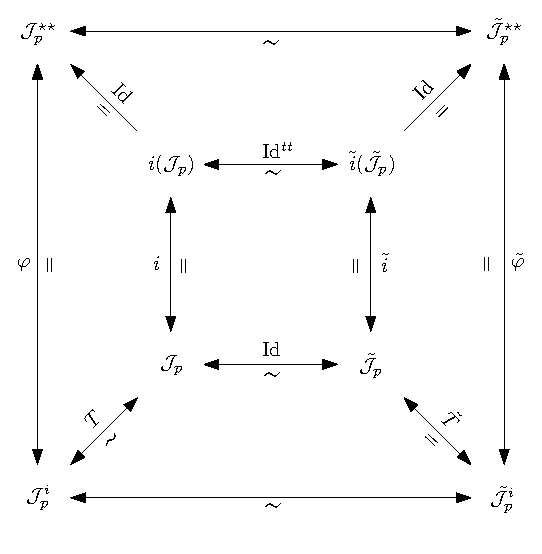
\includegraphics[width = 8.9cm,height=8.9cm]{james/isometrie.eps}}
\end{tabular}

\chapterref 

Ce chapitre prend sa source dans l'exercice 7 laiss� par Bernard Beauzamy, dans le chapitre sur les bases de Schauder (voir \cite[p. 97]{BEAUZAMY}). La section concernant la norme rendant l'espace de James isom�trique � son bidual est inspir�e de l'article de Robert Clarke James (voir \cite{JAMESISO}).


    \titleformat\chapter[hang]{\normalfont\huge\bfseries}{}{1em}{}
    \appendix{}

\chapter{Annexe}

Ici sont regroup�s certains r�sultats qui n'ont leur place dans aucun chapitre, mais qui sont n�cessaires � certaines d�monstrations.

\section{Th�or�mes de Hahn-Banach}

\begin{Thm}\label{HBF}
Dans un espace vectoriel norm�, toutes les applications du type $ev_x$ atteignent leur norme sur la boule unit�. Plus formellement,

\[
\forall x\in E, \exists\hspace*{0.1em}x\dual\in E\dual \text{ tel que }\norme{x\dual}=1\text{ et }x\dual(x)=\norme{x}
\]
\end{Thm}

\begin{Thm}\label{HBA}
Dans un espace vectoriel norm�, toute fonctionnelle continue d'un sous-espace s'�tend en une fonctionnelle continue de m�me norme sur l'espace tout entier.
\end{Thm}

\begin{Thm}
Soit $E$ un $\mathbb{R}$-espace vectoriel norm�. Soient $A\subseteq E$ convexe ferm� non vide, $B\subseteq E$ convexe compact non vide, tels que $A\cap B=\emptyset$. Alors il existe $x\dual\in E\dual$ et $\alpha\in\mathbb{R}$ tels que pour tout $a\in A, b\in B$,
\[x\dual(a)<\alpha<x\dual(b)\]
\end{Thm}

\begin{Corol}\label{HBC}
Soit $E$ un $\mathbb{K}$-espace vectoriel norm�. Soient $A$ et $B$ deux convexes ferm�s non vides disjoints de $E$ tels que l'un des deux est compact et $A$ est $\mathbb{K}$-sym�trique, c'est-�-dire que $\lambda A\subseteq A$, quelque soit $\lambda\in S(\mathbb{K})$. Alors il existe $x\dual\in E\dual$ et $\alpha>0$ tels que pour tout $a\in A, b\in B$,
\[\abs{x\dual(a)}<\alpha<\abs{x\dual(b)}\]
\end{Corol}
\begin{proof}
On consid�re $E$ un espace vectoriel r�el. Le th�or�me nous donne $x\dual\in E\dual$ et $\alpha\in\mathbb{R}$ tels que pour tout $a\in A, b\in B$,
\[\begin{array}{rrrrr}
x\dual(a)&<&\alpha &<&x\dual(b)\\
-x\dual(a)&>&-\alpha &>&-x\dual(b)\\
-x\dual(b)&<&-\alpha &<&-x\dual(a)
\end{array}\]
Ce qui indique que l'ordre des in�galit�s est ind�pendant du fait que ce soit $A$ ou $B$ le compact.

Soit $a\in A$, puisque $A$ est $\mathbb{R}$-sym�trique on a que $-a\in A$, et donc $0\leqslant\abs{x\dual(a)}<\alpha$. Par cons�quent, $\alpha>0$. Soit $b\in B$, on a que $0<\alpha<x\dual(b)\leqslant\abs{x\dual(b)}$. On en d�duit alors le corollaire pour un $\mathbb{R}$-espace vectoriel norm�.

Consid�rons maintenant $E$ un $\mathbb{C}$-espace vectoriel norm�, et notons $E_\mathbb{R}$ son �quivalent r�el. Appliquons le corollaire sur cet espace, on obtient alors $x_\mathbb{R}\dual\in E_\mathbb{R}\dual$ et $\alpha>0$ tels que pour tout $a\in A, b\in B, \abs{x_\mathbb{R}\dual(a)}<\alpha<\abs{x_\mathbb{R}\dual(b)}$. Le corollaire n'est pas encore d�montr�, puisque $x_\mathbb{R}\dual$ est $\mathbb{R}$-lin�aire, et donc pas n�cessairement $\mathbb{C}$-lin�aire. Par contre, si on d�finit $x\dual$ tel que pour tout $x\in E$,
\[
x\dual(x)=x_\mathbb{R}\dual(x)-ix_\mathbb{R}\dual(ix)
\]
on obtient bien une application de $E\dual$. Montrons que les in�galit�s souhait�es sont v�rifi�es aussi pour $x\dual$.

Soient alors $a\in A$ et $b\in B$. On a que
\[\abs{x\dual(b)}\geqslant\abs{\Re(x\dual(b))}=\abs{x_\mathbb{R}\dual(b)}>\alpha\]
De plus, $A$ est $\mathbb{C}$-sym�trique, donc il existe $\theta\in\mathbb{R}$ tel que $x\dual(a\e^{i\theta})>0$ et $a\e^{i\theta}\in A$. Par cons�quent,
\[
\abs{x\dual(a)}=\abs{x\dual(a\e^{i\theta})}=\abs{x_\mathbb{R}\dual(a\e^{i\theta})}<\alpha
\]
\end{proof}

Pour le th�or�me suivant, voir \cite[p. 29-31]{BEAUZAMY}.

\begin{Thm}\label{HBH}
Soient $E$ un espace vectoriel norm�, $L\neq\emptyset$ un sous-espace affin de $E$ et $\Omega\neq\emptyset$ un ouvert convexe de $E$. Si $L$ et $\Omega$ sont disjoints, alors il existe un hyperplan affin qui contient $L$ et qui ne rencontre pas $\Omega$.
\end{Thm}



\begin{Lemme}[Lemme alg�brique]\label{lemmealgebrique}
Soient $E$ un espace vectoriel norm�, $n\in\mathbb{N}_0$ et $x\dual, x\dual_1,...,x\dual_n\in E\dual$. Si $x\dual_1,...,x\dual_n$ sont lin�airement ind�pendants, alors les assertions suivantes sont �quivalentes:
\begin{enumerate}[(1)]
\item $x\dual\in\Span(x\dual_1,...,x\dual_n)$
\item $\bigcap\limits_{k=1}^n \ker(x\dual_k)\subseteq\ker(x\dual)$
\end{enumerate}
\end{Lemme}
\begin{proof}
~

(1) $\Rightarrow$ (2)\\
%
Puisque $x\dual\in\Span(x\dual_1,...,x\dual_n)$, il existe $a_1,...,a_n\in\mathbb{K}$ tels que $x\dual=\sum\limits_{k=1}^n a_k x\dual_k$. Soit $x\in\bigcap\limits_{i=k}^n \ker(x\dual_k)$. Alors
\[
x\dual(x)
=
\sum\limits_{k=1}^n a_k x\dual_k(x)
=
0
\]

(2) $\Rightarrow$ (1)\\
%
Soit l'application lin�aire
\[
\begin{array}{lllll}
\varphi&:&E&\maps&\mathbb{K}^{n+1}\\
&:&x&\mapsto&(x\dual(x),x\dual_1(x),...,x\dual_n(x))
\end{array}
\]
Son image est un sous-espace vectoriel ferm� de $\mathbb{K}^{n+1}$. Alors par le th�or�me de Hahn-Banach (\ref{HBC}), puisque $(1, 0, ..., 0)\notin \Image(\varphi)$, on peut s�parer $\{(1, 0, ..., 0)\}$ et $\Image(\varphi)$, autrement dit il existe $A\in (\mathbb{K}^{n+1})\dual$ et $\alpha>0$ tels que pour tout $x\in E$, on a
\[
\abs{A(\varphi(x))}<\alpha<\abs{A((1,0,...,0))}
\]
Cela signifie que $\Image(A\circ\varphi)$ est born�. Or c'est un espace vectoriel, donc il est r�duit � l'�l�ment nul. De plus, $A$ s'identifie � $(a,a_1,...,a_n)\in\mathbb{K}^{n+1}$, alors d'une part $A((1,0,...,0))=a\neq 0$ car $\alpha<\abs{A((1,0,...,0))}$, d'autre part pour tout $x\in E$ on a que
\[
A(\varphi(x))
=
a x\dual(x) + \sum_{k=1}^n a_k x\dual_k(x)
=
0
\]
Ce qui signifie que $x\dual$ est une combinaison lin�aire de $x\dual_1,...,x\dual_n$.
\end{proof}


\section{Espace quotient}

\begin{Def}\label{espaceortho}
Soient $E$ un espace vectoriel norm� et $F$ un sous-espace ferm� de $E$. On dit que l'espace vectoriel
\[
F\ortho=\{x\dual\in E\dual | x\dual(F)=\{0\}\}
\]
est l'espace orthogonal de $F$.
\end{Def}

\begin{Prop}\label{quotientbanach}
Soit $E$ un espace de Banach et $F$ un sous-espace ferm� de $E$. Alors l'espace vectoriel $E/F$ muni de la norme
\[
\begin{array}{lllll}
\norme{.}&:&E/F&\maps&\mathbb{R}^+\\
&:&x+F&\mapsto&\inf\limits_{f\in F}\norme{x+f}
\end{array}
\]
est un espace de Banach.
\end{Prop}

\begin{Prop}\label{ForthoisoEsurF}
Soit $E$ un espace de Banach et $F$ un sous-espace ferm� de $E$. Alors l'application
\[
\begin{array}{lllll}
\varphi&:&F\ortho&\maps&(E/F)\dual\\
&:&x\dual&\mapsto&\left(
    \begin{array}{lll}
    E/F&\maps&\mathbb{K}\\
    x+F&\mapsto&x\dual(x)
    \end{array}
\right)
\end{array}
\]
est une isom�trie.
\end{Prop}

\begin{proof}
En premier lieu, il faut s'assurer que $\varphi$ est bien d�finie, c'est-�-dire que pour tout $x\dual\in F\ortho$, $\varphi(x\dual)\in (E/F)\dual$. Soient $x\in E$, $f\in F$ et $x\dual\in F\ortho$. On a que $x\dual(x+f)=x\dual(x)$ car $x\dual$ s'annule sur $F$, donc l'image de $x+F$ par $\varphi(x\dual)$ ne d�pend pas du repr�sentant de classe choisi. La lin�arit� et la continuit� de $\varphi(x\dual)$ sont �videntes.

La lin�arit� de $\varphi$ est elle aussi �vidente.

L'application est continue. Soient $x\dual\in F\ortho$, $x\in E$ et $f\in F$. On a

\[
\abs{\varphi(x\dual)(x+F)}
=
\abs{x\dual(x)}
=
\abs{x\dual(x+f)}
\leqslant
\norme{x\dual}\norme{x+f}.
\]

Ce qui implique que $\abs{\varphi(x\dual)(x+F)}\leqslant \norme{x\dual}\norme{x+F}$. Par cons�quent, $\norme{\varphi(x\dual)}\leqslant\norme{x\dual}$ et $\varphi$ est continue.

On montre que $\varphi$ est surjective. Soit $\overline{x\dual}\in(E/F)\dual$. On prend

\[
\begin{array}{lllll}
x\dual&:&E&\maps&\mathbb{K}\\
&:&x&\mapsto&\overline{x\dual}(x+F)
\end{array}
\]

La lin�arit� de $x\dual$ est �vidente, montrons qu'elle est continue et de norme inf�rieure � $\norme{\overline{x\dual}}$, ceci nous donnera � la fois la surjectivit� et le caract�re isom�trique de $\varphi$. Soit $x\in E$. On a

\[
\abs{x\dual(x)}
=
\abs{\overline{x\dual}(x+F)}
\leqslant
\norme{\overline{x\dual}}\norme{x+F}
\leqslant
\norme{\overline{x\dual}}\norme{x}
\]

De plus, quelque soit $f\in F$, on a que $x\dual(f)=\overline{x\dual}(f+F)=\overline{x\dual}(0+F)=0$ donc $x\dual\in F\ortho$. La v�rification du fait que $\varphi(x\dual)=\overline{x\dual}$ est �vidente, donc $\varphi$ est surjective.
\end{proof}




\begin{Prop}\label{lipschitz}
Soient $E$ un espace vectoriel norm�, $c\in\mathbb{K}_0$ et $x\dual\in E\dual$ non nul. Alors, en posant $H=\inv{x\dual}(c)$, on a
\[
\sup_{x\in H}\frac{\abs{x\dual(x)}}{\norme{x}}
=
\sup_{\substack{x\in E\\x\neq 0}}\frac{\abs{x\dual(x)}}{\norme{x}}
=
\norme{x\dual}
\]
\end{Prop}

\begin{proof}
Soit $x\in H$, et soit $\alpha\in\mathbb{K}_0$. On a
\[
\sup_{x\in H}\frac{\abs{x\dual(x)}}{\norme{x}}
=
\sup_{x\in H}\frac{\abs{x\dual(x)}}{\norme{x}}\frac{\alpha}{\alpha}
=
\sup_{x\in H}\frac{\abs{x\dual(\alpha x)}}{\norme{\alpha x}}
=
\sup_{x\in\alpha H}\frac{\abs{x\dual(x)}}{\norme{x}}
\]

Puisque $H$ est le translat� d'un sous-espace de $E$ de codimension 1, on a que $\mathbb{K}_0 H$ et $\ker(x\dual)$ partitionnent $E$. On en d�duit que
\[
\sup_{x\in H}\frac{\abs{x\dual(x)}}{\norme{x}}
=
\sup_{\substack{x\in E\\x\neq 0}}\frac{\abs{x\dual(x)}}{\norme{x}}
\]

De plus,
\[
\sup_{\substack{x\in E\\x\neq 0}}\frac{\abs{x\dual(x)}}{\norme{x}}
=
\sup_{\substack{x\in S(E)\\ \alpha>0}}\frac{\abs{x\dual(\alpha x)}}{\norme{\alpha x}}
=
\sup_{\substack{x\in S(E)\\ \alpha>0}}\frac{\alpha \abs{x\dual(x)}}{\alpha \norme{x}}
=
\sup_{x\in S(E)}\abs{x\dual(x)}
=
\norme{x\dual}
\]
\end{proof}

%\begin{Thm}[James]
Dans un espace de Banach, les assertions suivantes sont �quivalentes:
\begin{enumerate}[(1)]
\item L'espace est r�flexif
\item Toute fonctionnelle atteint sa norme sur la boule unit�
\end{enumerate}
\end{Thm}

\begin{proof}
(1) $\Rightarrow$ (2)\\
Soit $x\dual\in E\dual$. Par le th�or�me de Hahn-Banach (\ref{HBF}), il existe $x\bidual\in E\bidual$ tel que $\norme{x\bidual}=1$ et $x\bidual(x\dual)=\norme{x\dual}$. Comme $E$ est r�flexif, il existe $x\in E$ tel que $ev_x=x\bidual$, et $\norme{x}=\norme{ev_x}=1$. Donc $x\dual(x)=x\bidual(x\dual)=\norme{x\dual}$.

(2) $\Rightarrow$ (1): voir \cite[p. 205-216]{JAMESF}.
\end{proof}



    \begin{thebibliography}{999}

\bibitem{BEAUZAMY} Bernard Beauzamy,
\textit{Introduction to Banach spaces and their geometry},
North Holland, seconde r�vision (1985).

\bibitem{BREZIS} Ha�m Br�zis,
\textit{Analyse fonctionnelle: th�orie et applications},
Masson, deuxi�me tirage (1987).

\bibitem{MONTESINOS} Mari�n Fabian et al.,
\textit{Functional Analysis and Infinite-Dimensional Geometry},
Springer (2001).

\bibitem{CONVINCOND} Christopher Heil,
\textit{A Basis Theory Primer},
Unexpanded Edition, Birkh�user, Boston (2011).

\bibitem{EBERLEINSMULIAN} Nelson Dunford, Jacob Theodore Schwartz,
\textit{Linear Operators. Vol. 1},
Pure and Applied Mathematics, Interscience Publishers (1963).

\bibitem{PENFLO} Per Henrik Enflo,
\textit{A counter-example to the approximation problem in Banach spaces},
Acta Math., 130 (1973).

\bibitem{JAMESF} Robert Clarke James,
\textit{Reflexivity and the supremum of linear functionals},
Ann. of Maths, 66 (1957).

\end{thebibliography}

\batchmode
\end{document}
